\documentclass[a4paper,12pt]{tesiinfo}
%\documentclass[a4paper,12pt,dvipdfm]{tesiinfo}

\usepackage{amsfonts}
\usepackage{amsmath}
\usepackage{latexsym}
\usepackage{tabularx}
\usepackage[italian]{babel}
\usepackage[bookmarks=true]{hyperref}
\usepackage{subfigure}
\usepackage{graphicx}
\usepackage{amssymb}

%FROM UNI - NOT INCLUDED IN BASIC COMMANDS
\usepackage{fncychap}

%ADDS SYMBOLS FOR MATH OPERATIONS: CEIL and FLOOR
\usepackage{mathtools}
\DeclarePairedDelimiter\ceil{\lceil}{\rceil}
\DeclarePairedDelimiter\floor{\lfloor}{\rfloor}

%EQUISPACES THE FRACTIONS
\usepackage{multicol}
\usepackage{fixmath}
\newcommand\ddfrac[2]{\frac{\displaystyle #1}{\displaystyle #2}}

%DISPLAY IMAGES CORRECTLY
\usepackage[export]{adjustbox}
\graphicspath{ {Images/} }
\usepackage{float}

%PSEUDO ALGORITMI
\usepackage{algorithm}
\usepackage{algpseudocode} 


%\usepackage[export]{algorithm}
%\usepackage[export]{algorithmic}
%\usepackage{caption}
%\newlength\myindent
%\setlength\myindent{2em}
%\newcommand\bindent{%
%%  \setlength{\itemindent}{\myindent}
%  \addtolength{\algorithmicindent}{\myindent}
%}
%\newcommand\eindent{\endgroup}

%FOOTNOTES - FONT SIZE DECREASED. Non usato...
%\usepackage{lmodern}

%9pt \`e la dimensione del font footnote
%11pt \`e la spaziatura. Se impostato a <9pt=troppo piccolo, se >12pt= troppo grande
\renewcommand{\footnotesize}{\fontsize{9pt}{11pt}\selectfont}

%Imposta 9 simboli diversi per creare le note. Cos\`i evitiamo di confondere "le note" con "la notazione usata". Tuttavia non sembrano "professionali" o adatti ad una tesi e sono in numero limitati a 9 per capitolo (cambiare capitolo resetta il contatore dei simboli).
%1 - *
%2 - †
%3 - ‡
%4 - §
%5 - ¶
%6 - ||
%7 - ∗∗
%8 - ††
%9 - ‡‡
%\renewcommand{\thefootnote}{\fnsymbol{footnote}}
\renewcommand{\thefootnote}{\Roman{footnote}}

%BOH
\hypersetup{final}

%Per mettere liste con a), b) ecc
\usepackage{enumitem}

%Inserire pagine bianche con il comando \afterpage{\blankpage}
\usepackage{afterpage}

\newcommand\blankpage{%
    \null
    \thispagestyle{empty}%
    \addtocounter{page}{-1}%
    \newpage}


\titolo{Crittografia Ellittica}
\laureando{Marco Carolla}
\relatore{Gabriele Di Stefano}
\annoaccademico{2016-2017}

\begin{document}

%\maketitle %Aggiunge la pagina iniziale dell'università
\contentspage %Aggiunge l'indice

%\pagenumbering{Roman}
%\listoffigures
%\listoftables
%\pagenumbering{arabic}


\chapter{Introduzione alla Sicurezza Informatica}
Con la parola composta da ``\textit{scritto}" e ``\textit{grafia}" intendiamo quella tematica della sicurezza in generale che mira ad una scrittura segreta, tale che non possa essere letta senza conoscere l'artificio usato nella corrispondenza. Parliamo di scrittura cifrata quando il risultato della lettura di un testo \`e privo di significato apparente. La cifratura di un testo pu\`o essere fatta per:
\begin{itemize}
 \item ``\textit{trasposizione}" mediante la quale la traduzione del linguaggio chiaro in linguaggio segreto ha luogo con spostamento o inversione degli elementi in chiaro
 \item ``\textit{sostituzione}" degli elementi del linguaggio con segni convenzionali che pur potendo essere di qualsiasi genere, sono in pratica quelli della normale scrittura, lettere o cifre
 \item ``\textit{sistema misto}" che combina le precedenti interponendole una dopo l'altra
\end{itemize} 
Un esempio di crittografia lo troviamo nell'Antica Grecia per opera di Polibio. La sua idea di crittografia consisteva nel disporre le lettere dell'alfabeto in una matrice avente righe e colonne numerate, questo sistema prende il nome di \textit{Scacchiera di Polibio}. L'impostazione base vede rappresentate le 26 lettere dell'alfabeto in questa scacchiera di 5 righe e 5 colonne, con la premura di porre due lettere (diciamo \textit{J} e \textit{K}) all'interno della stessa casella. Il carattere cifrato corrisponde alla coppia riga-colonna determinata dalla lettera in chiaro: oggi viene adottato un sistema analogo per far riferimento agli elementi di una matrice. L'utilizzo di questo metodo fa corrispondere al testo in chiaro ``\textit{Polibio}" il testo cifrato ``\emph{35 34 31 24 12 24 34}". 
\\
Pochi anni pi\`u tardi, a Roma, l'imperatore Cesare ide\`o un sistema trasposizione oggi noto come \textit{cifrario di Cesare} facente uso di un singolo alfabeto per crittografare il testo, esso \`e quindi un sistema \textit{Monoalfabetico}. Utilizzare questo cifrario con una trasposizione di 3 caratteri significa che il testo in chiaro ``\textit{Cesare}" corrisponder\`a al testo cifrato ``\textit{Fhzdvh}".
\\
Intorno al 16$^\circ$ secolo venne introdotto un sistema \textit{Polialfabetico} facente uso di una variante del cifrario di Cesare nel quale la trasposizione non \`e pi\`u rappresentata da un alfabeto ``\textit{ordinato}", bens\`i abbiamo ora una serie di simboli presi da molteplici alfabeti. La chiave di questo sistema consiste nel conoscere l'ordine della sequenza di tali simboli.
\\
\\
L'evoluzione continua della tecnologia ha fatto emergere il bisogno di algoritmi crittografici ben pi\`u all'avanguardia di quelli appena descritti. L'avvento di internet ha favorito lo scambio di messaggi per via telematica: il messaggio viene inviato al destinatario grazie ai protocolli della pila ISO/OSI e vi arriva passando per mezzi di comunicazione non sicuri. La ``non sicurezza" del canale di comunicazione costituisce un problema sulla \textit{riservatezza} della comunicazione e sul \textit{riconoscimento dell'interlocutore}: se esiste la possibilit\`a di intercettare ed inviare messaggi, allora chiunque pu\`o mascherarsi da interlocutore ed inviare messaggi sotto falso nome. Giungiamo quindi a parlare di algoritmi crittografici con i quali intendiamo la trasformazione reversibile di un testo, rendendolo decifrabile solo a chi dispone di opportune informazioni dette \textit{chiavi crittografiche}. 
\\
Per crittografare un messaggio $m$ mediante algoritmi di crittografia definiamo le funzioni ``$E(m,K)$" per la cifratura e ``$D(c, K)$" per la decifratura. Quando viene applicata $E(\cdot )$ al messaggio $m$ si ottiene il messaggio cifrato ``$c$" per mezzo di una chiave $K$. La reversibilit\`a di tali funzioni si basa sulla stessa $K$ (od una diversa per algoritmi pi\`u complicati descritti in seguito). In definitiva abbiamo le due relazioni 
\begin{align*}
    \begin{cases}
     c= E(m, K)  &\text{Cifratura di $m$ in $c$}\\
     m= D(c, K)  &\text{Decifratura di $c$ in $m$}
    \end{cases}
\end{align*}
Le chiavi sono sostanzialmente numeri pseudo-casuali molto grandi, la cui lunghezza si misura in bit: maggiore \`e la lunghezza della chiave, pi\`u saranno onerose le operazioni di cifratura e decifratura. Essendo ciascun protocollo di crittografia aperto e \textbf{noto} a tutti, la chiave assume un ruolo critico nella sicurezza: chiunque conosca quella di decifratura pu\`o decrittare e leggere il messaggio.
\\
In definitiva classifichiamo gli algoritmi di cifratura in \textit{Reversibili} ed \textit{Irreversibili}. I primi si suddividono a loro volta in due classi di algoritmi: quelli simmetrici (che necessitano di una singola chiave crittografica) e quelli asimmetrici (per i quali abbiamo bisogno di due chiavi). Gli algoritmi irreversibili vengono dati dall'applicazione di funzioni di hash.
%
%
%
\section{Crittografia Simmetrica}
Gli algoritmi crittografici reversibili sono alla base della crittografia simmetrica. Consideriamo il messaggio in chiaro $m$ crittografato mediante l'algoritmo $S_c$ e chiave $K^S$; ottenere nuovamente il messaggio $m$ \`e un'operazione possibile mediante l'applicazione dell'algoritmo $S_d$ al messaggio crittografato, utilizzando la \textbf{stessa chiave} $K^S$ usata in fase di cifratura. L'esempio reale che spiega questo funzionamento viene descritto di seguito: due utenti della rete, detti Alice e Bob, decidono di scambiarsi messaggi sulla rete internet e, per farlo, optano per una crittografia simmetrica dei loro dati. I passi necessari ad instaurare una comunicazione sicura tra i due si fonda sui seguenti passaggi: 
\begin{enumerate}
 \item Concordare i due algoritmi $S_c$ e $S_d$ complementari. L'idea della complementariet\`a corrisponde a dire che, calcolato un messaggio cifrato come $C = S_c(m, K)$, allora si potr\`a riottenere il messaggio originale applicando $m = S_d(C, K)$
 \item Concordare la chiave $K^S$. Entrambi Alice e Bob avranno a disposizione la medesima chiave per le operazioni di cifratura e decifratura. Per questo motivo, la chiave viene denominata \textit{simmetrica}
 \item Alice, per mandare il suo messaggio $m_A$ a Bob, procede nell'applicare l'algoritmo di crittografia con la chiave simmetrica, ovvero calcola $C_A = S_c(m_A, K^S)$ ed invia quest'ultimo sul canale non sicuro
 \item Bob riceve il messaggio crittato $C_A$, applica l'algoritmo di decrittazione con la chiave simmetrica ed ottiene il messaggio in chiaro di Alice: 
 \begin{center}
  $S_d(C_A$, $K^S) = S_d[S_c(m_A$, $K^S)$, $K^S] = m_A$
 \end{center}
\end{enumerate}
La chiave $K^S$, unica per entrambi gli interlocutori, determina la sicurezza della crittografia simmetrica, di conseguenza rappresenta la difficolt\`a computazionale nel decifrare il messaggio crittato qualora non si disponga di essa. 
\\
Ricordando che la cifratura di un messaggio avviene per trasposizione e sostituzione, le operazioni di cifratura e decifratura necessitano di un tempo computazionale proporzionale alla lunghezza del messaggio ed alla lunghezza in bit della chiave crittografica. Una chiave di lunghezza in bit contenuta, permette un'elevata velocit\`a nella cifratura e decifratura del messaggio, a discapito della sicurezza dall'algoritmo. Mantenere un equilibrio tra velocit\`a e sicurezza offerta non \`e un compito banale pertanto gli algoritmi della crittografia simmetrica sono adatti a trattare messaggi di grandi dimensioni affidandosi ad una chiave di lunghezza contenuta, a patto che questa sia nota solo ed esclusivamente agli interlocutori. D'altronde non si \`e detto \textbf{come} Alice e Bob siano giunti a concordare la medesima chiave: se tutta la segretezza della comunicazione si basa sulla chiave $K^S$ condivisa, come si scambia tale chiave in modo sicuro?
%
%
%
%
%
%
%
%
%
%
\section{Crittografia Asimmetrica}
Il problema dello scambio della chiave simmetrica $K^S$ viene risolto dalla crittografia asimmetrica, concetto nato nel 1976 per merito di Whitfield Diffie e Martin Hellman. Oggi, il pi\`u noto e diffuso algoritmo della crittografia a chiave pubblica \`e RSA\footnote{\footnotesize{Il nome \`e dato dalle iniziali dei tre ricercatori del MIT: Ron \textbf{R}ivest, Adi \textbf{S}hamir, Leonard \textbf{A}dleman}}. L'idea alla base di questa crittografia prevede che un utente della rete generi una \textit{coppia di chiavi complementari}, una chiave \`e detta \textbf{pubblica} $K^+$ e l'altra \`e detta \textbf{privata} $K^-$. La chiave pubblica $K^+$ viene scambiata dai due interlocutori, mentre quella privata $K^-$ viene mantenuta segreta. 
\\
La matematica alla base della crittografia asimmetrica determina che, data la coppia di chiavi complementari $(K^-, K^+)$, il testo cifrato tramite $K^+$ possa essere decifrato esclusivamente dalla corrispondente $K^-$. Per mantenere alta la segretezza delle informazioni, la conoscenza della chiave pubblica non deve consentire il calcolo di quella privata. 
\\
Dati Alice e Bob, due utenti della rete che vogliono scambiarsi informazioni in modo riservato, si procede nel seguente modo:
\begin{enumerate}
 \item Alice genera coppia di chiavi $({K_A}^-, {K_A}^+)$, Bob genera la coppia $({K_B}^-, {K_B}^+)$
 \item Si procede allo scambio delle chiavi pubbliche. Alice \`e ora in possesso di $({K_A}^-, {K_A}^+, {K_B}^+)$ mentre Bob ha $({K_B}^-, {K_B}^+, {K_A}^+)$. Si ricorda che gli scambi avvengono sempre su un canale non sicuro e che, quindi, tale chiave pubblica pu\`o essere intercettata da terzi
 \item Alice pu\`o ora mandare il suo messaggio $m_A$ cifrandolo con la chiave \textbf{pubblica} di Bob: $C_A = {K_B}^+(m_A)$
 \item Bob riceve il messaggio $C_A$ e pu\`o decifrarlo in quanto conosce la chiave privata, complementare, corrispondente:
 \begin{center}
 ${K_B}^-(C_A) = {K_B}^-({K_B}^+(m_A)) = m_A$
 \end{center}
\end{enumerate}
La complementariet\`a delle chiavi permette l'integrit\`a dei messaggi scambiati. L'uso di una chiave pubblica, che pu\`o essere nota a tutti, per crittografare un messaggio, richiede una lunghezza in bit maggiore rispetto a quella usata negli algoritmi simmetrici. Da ci\`o deriva un aumento della complessit\`a computazionale e dei tempi di calcolo non solo per la generazione delle chiavi ma soprattutto per le operazioni di cifratura e decifratura del messaggio.
\\
Gli algoritmi asimmetrici costituiscono quindi un'alternativa pi\`u sicura rispetto quelli simmetrici ma risultano essere fortemente inefficienti per trattare documenti di grossa dimensione: sono significativamente pi\`u lenti di qualsiasi algoritmo simmetrico.
%
%
%
%
%
%
%
%%
%
%
%
%
%
%
\section{Crittografia Ibrida}
\label{critt ibrida}
Se gli algoritmi asimmetrici permettono un'elevata sicurezza e quelli simmetrici favoriscono il tempo computazionale, unire i vantaggi dei due sistemi di crittografia visti d\`a vita alla ``\textit{Crittografia Ibrida}". In questo caso, i due interlocutori Alice e Bob agiranno come segue:
\begin{enumerate}
 \item Alice genera la coppia di chiavi $({K_A}^-, {K_A}^+)$, Bob genera la coppia $({K_B}^-, {K_B}^+)$
 \item Si procede allo scambio delle chiavi pubbliche. Alice \`e ora in possesso di $({K_A}^-, {K_A}^+, {K_B}^+)$ mentre Bob ha $({K_B}^-, {K_B}^+, {K_A}^+)$
 \item Chi dei due voglia iniziare la comunicazione genera la chiave simmetrica $K^S$. Poniamo il caso che Alice sia a generarla, le chiavi in suo possesso sono quindi $({K_A}^-, {K_A}^+, K^S, {K_B}^+)$
 \item Ella procede nel cifrare il suo messaggio $m_A$ con la chiave \textbf{simmetrica} $K^S$ ottenendo $C_A = K^S(m_A)$. Stiamo ora parlando di crittografia simmetrica, rendendo possibile lo scambio di messaggi molto grandi
 \item Inoltre, Alice dovr\`a anche cifrare la propria chiave simmetrica con quella pubblica di Bob ottenendo $k_A={K_B}^+(K^S)$ in modo che Bob abbia la possibilit\`a decifrare prima la chiave simmetrica e quindi il messaggio. Ci\`o che Alice invier\`a \`e la coppia $(C_A, k_A)$
 \item Bob riceve la coppia $(C_A, k_A)$ e procede nel decifrare la chiave simmetrica di Alice applicando la propria chiave privata 
 \begin{center}
  ${K_B}^-(k_A)={K_B}^-[{K_B}^+(K^S)]=K^S$
 \end{center}
 La correttezza di quanto calcolato \`e il fondamento della crittografia asimmetrica.\\
 Egli si trova ora in possesso della chiave simmetrica generata da Alice con la quale pu\`o decifrare il messaggio $C_A$ applicando il fondamento della crittografia simmetrica:
 \begin{center}
  ${K}^S(C_A)={K}^S({K}^S(m_A))=m_A$
 \end{center}
\end{enumerate}
L'approccio appena visto usa la crittografia asimmetrica per crittografare, decrittare ed inviare una chiave simmetrica, condivisa tra i due interlocutori. La sicurezza e l'integrit\`a delle informazioni sono le stesse della crittografia asimmetrica ed i tempi di computazione risultano ridotti grazie al principio crittografia simmetrica.
\\
\\
Un importante fattore che si \`e tralasciato fino a questo punto \`e la verifica di autenticit\`a dell'interlocutore. Tutti gli scambi di chiave effettuati sono tra Alice e Bob, due persone distanti tra loro che non possono accertarsi ``\textit{di persona}" sul loro effettivo interlocutore. Come pu\`o procedere Bob qualora volesse verificare che il suo interlocutore sia effettivamente Alice? Il metodo adottato per verificare l'autenticit\`a delle parti in gioco \`e detto Firma Digitale e si basa sul principio della crittografia asimmetrica.
%
%
%
\section{Firma Digitale}
L'utente Bob richiede che Alice dimostri la sua autenticit\`a prima di procedere allo scambio di messaggi ed ogni volta che egli lo riterr\`a opportuno. La firma digitale di Alice si compone dei seguenti passaggi: 
\begin{enumerate}
 \item Alice genera coppia di chiavi $({K_A}^-, {K_A}^+)$;
 \item Cifra il suo messaggio $m_A$ con la chiave propria chiave \textbf{privata} ottenendo
 \begin{center}
 $C_A = {K_A}^-(m_A)$
 \end{center}
 La sua firma digitale sar\`a quindi la terna $F_A = (C_A, m_A, {K_A}^+)$
 \item Invia quindi la firma digitale, sul canale non sicuro, a Bob
\end{enumerate}
In questo momento tutti possono dire che se, applicando la chiave \textit{pubblica} di Alice, vale l'uguaglianza ${K_A}^+(C_A) = m_A$ allora Alice \`e effettivamente chi dice di essere.
\\
Il problema di fondo \`e ancora l'inefficienza degli algoritmi asimmetrici per gestire il messaggio $m_A$. Si considera quindi una soluzione alternativa per gestire le firme digitali: l'utilizzo delle funzioni di hash, particolari funzioni matematiche unidirezionali (\textit{one-way}), che prendono in input il messaggio in chiaro e restituiscono un numero la cui lunghezza in bit \`e determinata dall'algoritmo di hash utilizzato (comunemente 128 o 160 bit). Il valore di output \`e detto \textit{impronta} o \textbf{hash} del messaggio e costituisce una vera e propria impronta digitale poich\`e l'hash non \`e computazionalmente invertibile, ossia data l'impronta \`e molto difficile risalire al testo originale. Tuttavia, per quanto difficile sia, l'hash \`e soggetto a collisioni, debolezza data dal restituire un output a lunghezza fissa nonostante input di lunghezza variabile, solitamente molto pi\`u lunga dell'output. Si parla quindi di ``\textit{collisione}" qualora due messaggi diversi portino al medesimo hash. Le principali funzioni di hash: SHA-1\footnote{\footnotesize{Deprecato dopo il 2011 dal NIST, \textbf{N}ational \textbf{I}nstitute of \textbf{S}tandards and \textbf{T}echnology, e dopo la confermata collisione tramite l'esperimento \textbf{SHAttered} della Google \cite{Shattered}}}, SHA-256, MD5.
\\ 
\\
Il paradigma della Firma Digitale diventa, pertanto, il seguente: 
\begin{enumerate}
 \item Alice genera la coppia di chiavi $({K_A}^-, {K_A}^+)$
 \item Calcola l'hash del suo messaggio $m_A$ tramite l'algoritmo di hash $H$ ottenendo $C_A = H(m_A)$
 \item Critta tale hash mediante la sua chiave privata ${K_A}^-$ ottenendo infine
 \begin{center}
  $s = {K_A}^-(C_A) = {K_A}^-[H(m_A)]$
 \end{center}
 La sua firma digitale sar\`a quindi la terna $F_A = (s, C_A, {K_A}^+)$
 \item Invia la firma digitale, sul canale non sicuro, a Bob
\end{enumerate}
Sulla base del messaggio $C_A$, andiamo ad applicare la chiave pubblica di Alice al parametro $s$:
\begin{center}
 ${K_A}^+(s) = {K_A}^+[{K_A}^-(C_A)] = C_A$
\end{center}
Il confronto tra i due messaggi cifrati, quello computato e quello ricevuto, determina se Alice sia effettivamente chi dice di essere. Infine il messaggio in chiaro viene ora mascherato dal suo hash rendendolo non pi\`u decifrabile da terzi: si \`e quindi aumentata la riservatezza del messaggio ed accelerati i tempi di calcolo.
%
%
%
%%
%
%
%
%
%
%
%%
%
\chapter{Nozioni fondamentali di Algebra}
Una \textbf{curva} nel linguaggio matematico \`e sinonimo di linea. Si parla non di curva in senso assoluto, ma di tipi di curve (come curva continua, curva piana, curva liscia), ciascuno dei quali \`e rigorosamente definito \cite{curva3c}.
\\
Lo studio di una curva si effettua su di un Campo $K$: insieme di elementi, non vuoto, sul quale vengono definite le operazioni binarie della somma e del prodotto e le loro operazioni inverse, sottrazione e divisione. I campi pi\`u noti sono quelli dei numeri naturali $\mathbb{N}$, dei reali $\mathbb{R}$, dei complessi $\mathbb{C}$. Campi con un numero finito di elementi sono detti ``\textit{Campi finiti}" o anche ``\textit{Campi di Galois}", vengono rappresentati dalle notazioni, equivalenti tra loro:  $\mathbb{F}_{n^m} = \mathbb{Z}/{n^m}\mathbb{Z} = \{0, 1, \ldots, n-1\}$; con $n$ un numero primo, $m$ un numero naturale maggiore o uguale ad 1. I campi della forma $\mathbb{F}_{2^m}$ vengono detti ``\textit{campi binari}", quelli invece definiti come $\mathbb{F}_{n}$ vengono detti ``\textit{campi primi}". Il numero di elementi del campo \`e pari ad $n$, detto \textbf{ordine}.
\\
Ciascun campo ha una \textbf{caratteristica} definita secondo la seguente formula:
\begin{gather}
n \in \mathbb{N}\text{, }n \ne 0 \text{, }char(\mathbb{F}_{n^m}) = \begin{cases} \min (n) \mid \underbrace{1+1+\cdots+1}_\text{n volte} = 0 & \mbox{se }\exists n\\
0 & \mbox{altrimenti}\\
\end{cases}
\label{charField}
\end{gather}
la caratteristica \`e pari al minimo numero di volte che l'elemento identit\`a della somma (\textbf{1}) deve essere sommato a se stesso per ottenere l'elemento identit\`a della moltiplicazione (\textbf{0}). Se non fosse possibile definire tale $n$ si assume la caratteristica pari a \textit{zero}. 
\\
Per un campo finito, l'ordine e la caratteristica coincidono. Si pu\`o dimostrare che il numero $n$ debba essere \textit{primo} procedendo per assurdo: se esso non fosse primo permetterebbe una scomposizione del tipo $n=n_1 \cdot n_2$, dove $n_1>1$ ed $n_2>1$ allora:
\begin{center}
 $0=\underbrace{1+1+\cdots+1}_\text{n} = \underbrace{(1+1+\cdots+1)}_{n_1} \cdot \underbrace{(1+1+\cdots+1)}_{n_2}$
\end{center}
Dato che il termine centrale \`e pari a 0 per definizione di caratteristica, almeno uno dei due termini a destra deve corrispondere a 0 ma ci\`o \`e assurdo in quanto $n$ \`e gi\`a il numero minimo per soddisfare tale relazione. I due fattori scelti $n_1$ ed $n_2$ verificherebbero l'uguaglianza solo nei casi $n_1=1$, $n_2=n$ o viceversa $n_1=n$, $n_2=1$ ma il valore ``\emph{1}" \`e stato escluso nell'ipotesi iniziale. Non esistendo quindi tali due numeri $n_1$ ed $n_2$ tali che il loro prodotto sia $n$ si deduce la primalit\`a di quest'ultimo.
\\
I campi $\mathbb{Q}$, $\mathbb{R}$ e $\mathbb{C}$ hanno caratteristica $0$.
\section{Gruppi}
\label{base gruppi}
Dati un insieme $G$ ed una funzione ``$\bullet$" definita come operazione binaria per la quale valga la propriet\`a della \textit{chiusura}
\begin{center}
 $(a, b) \to a \bullet b : G \times G \to G$
\end{center}allora la coppia $(G, \bullet)$ prende il nome di \textbf{gruppo} qualora vengano rispettati gli \textit{assiomi di gruppo}:
\begin{enumerate}
 \item \textit{Associativit\`a}: $\left ( a\bullet b \right ) \bullet c = a \bullet \left ( b \bullet c \right ) $, $ \forall (a, b, c) \in G$;
 \item \textit{Esistenza dell'identit\`a}: $ \exists ! e \in G \mid e \bullet a = a \bullet e = a$;
 %
 \item \textit{Esistenza dell'inverso}: $\exists b \in G \mid a \bullet b = b \bullet a = e$.
\end{enumerate} 
La funzione ``$\bullet$" definita prende il nome di \textbf{Legge del Gruppo G} ma viene solitamente omessa nel far riferimento ad un gruppo. Il tipo di Legge influenza come gli elementi interni vengono combinati tra loro: un gruppo \`e \textit{additivo} se la Legge \`e definita come ``somma" e l'elemento identit\`a \`e lo \emph{0}, alternativamente un gruppo \`e detto \textit{moltiplicativo} se tale Legge \`e una ``moltiplicazione" e l'elemento identit\`a \`e \emph{1}.\\
Agli assiomi di gruppo possiamo aggiungere la propriet\`a commutativa: se \`e vero che \begin{center}
 $ a \bullet b = b \bullet a$, $ \forall a, b \in G$
\end{center} 
allora il gruppo $G$ \`e detto \textit{Gruppo Abeliano}.
\\
\\
Parliamo di \textbf{sottogruppo} $S$ quando ci riferiamo ad un \textbf{sottoinsieme non vuoto} del gruppo $G$ per il quale valgano le condizioni
\begin{center}
$S \subset G \iff
    \begin{cases}
        a \bullet b \in S \text{ } &\forall a, b \in S\\
        a^{-1} \in S \text{ } &\forall a \in S
    \end{cases}$
\end{center}
dove con il termine ``$a^{-1}$" si intende l'elemento inverso di $a$ \cite{baseTheory_GT}.
\\
Parliamo di \textbf{ordine} di un gruppo quando facciamo riferimento alla sua cardinalit\`a (il suo numero di elementi), le notazioni usate sono $\mid G \mid$ oppure $\#G$. I sottogruppi di $G$ con ordine $\mid S \mid < \mid G \mid$ sono detti ``sottogruppi propri".
\\
Una propriet\`a molto importante per i sottogruppi discende dal \textit{Teorema di Lagrange} il quale afferma che ``\emph{la cardinalit\`a di un sottogruppo $H$ del gruppo $G$ \`e un \textbf{divisore intero} della cardinalit\`a di $G$}". In termini meno formali, se il gruppo $G$ ha cardinalit\`a $N$ ed uno dei suoi sottogruppi ha cardinalit\`a $n$ allora il rapporto $m = N \big / n$ \`e un numero intero $m \in \mathbb{Z}$ detto \textbf{cofattore}.
%
%
%
%
%
%
\\
\\
Un gruppo $G$ viene definito \textbf{ciclico} qualora sia generato a partire da un singolo elemento $g \in G$ per il quale si rispetti la relazione 
\begin{align*}
 &G= \{0, g, 2g, \ldots, (n-1)g\}& \text{ con }&ng=0& &\text{notazione \textit{Additiva}}\\
 &G= \{1, g, g^2, \ldots, g^{n-1}\}& \text{ con }&g^n=1& &\text{notazione \textit{Moltiplicativa}}
\end{align*}
ovvero ogni altro elemento del gruppo pu\`o essere ottenuto applicando ripetitivamente la Legge di Gruppo o la sua inversa all'elemento $g$.\\
L'elemento $g$ viene quindi detto \textbf{generatore} del gruppo $G$, ha un \textbf{ordine} indicato con la notazione $\langle g \rangle$ e corrisponde al pi\`u piccolo numero $m$ tale che $g^m = 1$ (in notazione Moltiplicativa) oppure tale che $mg = 0$ (in notazione Additiva) se tale $m$ esiste, altrimenti \`e infinito (a tal proposito vedasi la formula (\ref{ordineGeneratoreGruppo}) seguente):
\begin{gather}
m \in \mathbb{N}\text{, }m \ne 0 \text{, }\langle g \rangle = 
\begin{cases} 
\min (m) \mid mg = 0 & \mbox{se }\exists m \text{, notazione \textit{Additiva}}\\
\min (m) \mid g^m = 1 & \mbox{se }\exists m \text{, notazione \textit{Moltiplicativa}}\\
\infty & \mbox{altrimenti}\\
\end{cases}
\label{ordineGeneratoreGruppo}
\end{gather}
Per gruppi ciclici l'ordine del generatore $g$ e l'ordine del suo gruppo $G$ coincidono \cite{char_Ring}.
\\
Il campo dei numeri interi $\mathbb{Z}$ forma un Gruppo con legge ``+", elemento identit\`a 0, e gode della propriet\`a commutativa. Tale campo \`e quindi un \textit{Gruppo Additivo Abeliano}. \`E facile dimostrare che tale campo non possa essere un Gruppo Moltiplicativo poich\`e dato un qualsiasi elemento $z \in \mathbb{Z}$ il suo inverso sar\`a un numero razionale $q = 1 / z$, $q \in \mathbb{Q}$; al pi\`u abbiamo $q=1$ se scegliamo $z=1$ ma ci\`o non soddisferebbe tutti gli altri punti del campo.
\\
\\
Definiamo ora la tripla $(R, +, \cdot)$ con il termine ``anello" \cite{anelli1}: la sua coppia $(R, +)$ rappresenta un gruppo additivo abeliano, mentre l'operazione ``$\cdot$" segue le propriet\`a associativa e distributiva rispetto l'addizione, il suo elemento neutro $e=1$ viene definito come segue
\begin{center}
 $e\cdot a = a\cdot e = a$, $\forall a \in R$.%, $e \in R \setminus \{0\}$.
\end{center}
%
%
%
La caratteristica un anello $R$ \`e il pi\`u piccolo $n$ tale che valga la (\ref{charField}) per ogni suo elemento, pu\`o esser quindi definita come il \textit{minimo comune multiplo} delle caratteristiche di tutti i suoi elementi. Se tale minimo $n$ non esiste allora si assume che la caratteristica sia ``0" per definizione \cite{char_Ring}. Tutti gli anelli con caratteristica $char(R)=0$ sono \textit{infiniti}. 
L'unico anello con caratteristica $char(R)=1$ \`e l'anello banale, costituito da un solo elemento. 
Tutti gli anelli con caratteristica maggiore di $1$ sono costituiti da un numero finito di elementi. Suddivisioni dei numeri interi del tipo ``$\mathbb{Z}/n\mathbb{Z}$" forniscono anelli modulari con elementi in numero finito e caratteristica $char(R) = n$.
\\
Esempio di un sottogruppo generato da un anello modulare: detto $n$ un numero naturale diverso da zero, tutti i sottogruppi della forma $\mathbb{Z}/n\mathbb{Z}$ sono di ordine finito $n$ e contengono gli elementi
\begin{center}
 $H=\mathbb{Z}/n\mathbb{Z}=\{n\mathbb{Z}$, $ 1+n\mathbb{Z}$, $\ldots $, $(n-1)+n\mathbb{Z}$\}
 \\
\end{center}
preso, ad esempio $n=5$, il gruppo $H = \mathbb{Z}/5\mathbb{Z}$ comprender\`a, ciclicamente, gli elementi $H= \{0, 1, 2, 3, 4\}$.
%
%
%
\section{Spazio Proiettivo}
``Definito con $V$ uno spazio vettoriale, $\mathbb{P}$ \`e lo \textit{spazio proiettivo} costituito dai vettori monodimensionali dei sottospazi vettoriali di $V$. Se lo spazio vettoriale $V$ ha dimensione $n+1$, lo spazio proiettivo da esso generato avr\`a dimensione $n$" \cite{baseTheory_ProjSpace}.
\\
Possiamo pensare ad uno spazio proiettivo come ad un'estensione dello spazio Euclideo mediante l'aggiunta dei \textit{punti all'infinito}. A seconda dello spazio euclideo considerato, ad esempio una retta o un piano, si vengono a definire, nello spazio proiettivo, una retta proiettiva o un piano proiettivo.
\\
Estendere il piano Euclideo \cite{baseTheory_Euclid2Proj_Space} a quello proiettivo significa:
\begin{enumerate}
 \item per ogni classe di rette parallele, aggiungere un singolo nuovo punto. Tale punto \`e considerato come punto di incontro per ogni retta della stessa classe. Classi di diverse rette parallele avranno diversi punti. Questi punti sono chiamati \textit{punti all'infinito};
 \item aggiungere una nuova retta incidente su tutti e soli i punti all'infinito. Questa retta \`e chiamata \textbf{la} \textit{retta all'infinito}.
\end{enumerate}
Ne consegue l'esclusione dell'esistenza di rette proiettive parallele.
\\
Dato il punto $E=(x, y)$ nel piano Euclideo, la scrittura in \textit{coordinate omogenee} o ``\textit{coordinate proiettive}" \`e data da $E=[xZ:yZ:Z]$, con $Z \in \mathbb{R} \setminus \{0\}$ un numero reale diverso da zero.
\\
Riguardo la notazione: per distinguere le coordinate proiettive da quelle cartesiane, spesso vengono usate notazioni differenti da $(x, y)$. A volte viene sostituita la virgola ``\textbf{,}'' con il simbolo ``\textbf{:}'', altre volte le parentesi tonde ``\textbf{()}'' vengono sostituite da quadre ``\textbf{$\mathbb{[]}$}'' ed altre volte vengono usate entrambe le notazioni assieme; infine si \`e soliti preferire le lettere maiuscole per punti proiettivi. Esempio: coordinate cartesiane $(x, y) = (1, 4)$, omogenee $[X:Y:Z]=[1:4:Z]$. Per mantenere un evidente cambio di coordinate verr\`a usata quest'ultima notazione.
\\
\\
Diversamente da quanto accade per lo spazio Euclideo, due terne di coordinate omogenee rappresentano lo stesso punto se e solo se questo \`e ottenuto moltiplicando le coordinate per una costante diversa da 0. Ci\`o significa che, preso il punto sul piano cartesiano $(1, 2)$, questo pu\`o esser rappresentato dai punti omogenei $[1: 2: 1]$, $[2: 4: 2]$ o pi\`u in generale $[Z: 2Z: Z]$.
\\
Dal punto omogeneo $[X: Y: Z]$ otteniamo il punto cartesiano $(X/Z$, $Y/Z)$. Un caso degenere \`e per $Z=0$ per cui il punto rappresentato nello spazio proiettivo \`e il punto all'infinito $\mathcal{O} = [0: 1: 0]$. L'insieme di tutti i punti $[X: Y: 0]$, ovvero di tutti i punti all'infinito, \`e la retta all'infinito espressa con la notazione $[X:1:0]$ dove $X$ appartiene allo spazio proiettivo considerato. 
\\
\\
%
%
%
%\textbf{Spazio Affine}: struttura geometrica che generalizza quelle propriet\`a dello spazio Euclideo che sono indipendenti dai concetti di distanza e di misura degli angoli, mantenendo solo le propriet\`a di parallelismo e rapporto di lunghezze per segmenti paralleli. In uno spazio affine non viene distinto un punto di ``origine". Di conseguenza non possono esistere vettori con un'origine fissata e non possono essere univocamente associati ad un punto. In uno spazio affine esistono i vettori distanza (displacement vectors) anche chiamati \textit{traslazioni} tra due punti nello spazio. La dimensione di uno spazio affine \`e dunque pari alla dimensione dello spazio dei vettori di traslazione. Per uno spazio affine di dimensione uno $\mathbb{A}^1$ abbiamo una \textit{linea affine}, per uno spazio affine di dimensione due $\mathbb{A}^2$ abbiamo un \textit{piano affine}. \\ Gli spazi affini sono sottospazi degli spazi proiettivi: otteniamo un piano affine da un qualsiasi piano proiettivo rimuovendo la linea all'infinito ed i punti all'infinito. \`E quindi l'operazione inversa rispetto alla trasformazione dal piano euclideo a quello proiettivo. Similmente possiamo fare il passaggio inverso, ovvero costruire un piano proiettivo a partire da un piano affine aggiungendo la linea all'infinito e tutti i suoi punti. \\ \\
%
%
%
%Passiamo dunque ad esprimere il concetto di \textbf{variet\`a\footnote{\footnotesize{In inglese dette \textbf{Manifold}}}}: una variet\`a algebrica $V$ \`e l'insieme delle soluzioni di un sistema di polinomi sui numeri reali o complessi. Tramite le variet\`a algebriche \`e possibile creare un legame tra l'algebra e la geometria in modo tale da formulare problemi geometrici in termini algebrici e viceversa. Possiamo dunque dire che un punto del piano appartiene alla curva $C$ se le sue coordinate soddisfano l'equazione polinomiale data la cui soluzione \`e fornita dalla variet\`a algebrica. In una variet\`a algebrica $V$ chiamiamo il punto P \textit{singolare} se non pu\`o essere definita una tangente in quel punto. Per variet\`a definite sui reali il concetto di punto singolare generalizza il concetto di \textit{non derivabilit\`a}. Una variet\`a algebrica che non presenti punti singolari viene detta non singolare, \textit{liscia} o $\mathbb{C}^ {\infty}$ ed implica l'esistenza di derivate di ogni ordine. Classi di variet\`a algebriche sono le curve algebriche piane, le quali includono: rette, circonferenze, parabole, ellissi, iperbole, curve cubiche come ad esempio le curve ellittiche. \\ \\ 
%Definiamo una variet\`a affine $V$ su un campo chiuso $K$ come il luogo degli zeri in uno spazio affine $A^n$ $n$-dimensionale di una famiglia finita di polinomi in $n$ variabili con coefficienti in $K$ che generano un Ideale Primo. Alternativamente possiamo dire che, detta $V$ una variet\`a algebrica su un campo $K$, Diciamo che $V$ \`e una variet\`a affine se \`e data da un insieme di equazioni $f_j(x_1, \ldots , x_n) = 0$ $\forall j = 1, \ldots, m$ con coefficienti in $K$. \\ Esempio: chiamiamo $K$ un campo chiuso e $A^2$ lo spazio affine bidimensionale su $K$. I polinomi nell'anello $K[x, y]$ possono esser visti come funzioni a valori complessi su $A^2$ valutati nei punti di $A^2$. Il sottoinsieme S dell'anello che contiene un singolo elemento $f(x, y) = x + y - 1$. Il luogo degli zeri di $f(x, y)$ \`e l'insieme dei punti in $A^2$ sui quali la funzione si annulla, ovvero l'insieme di tutte le coppie di numeri complessi $(x, y)$ tali che $y = 1 - x$ (linea). L'insieme $V(f) = {(x, 1-x) \in C^2}$ \`e un sottoinsieme di $A^2$ ed un insieme algebrico. Tale insieme $V$ non \`e vuoto, \`e irriducibile dato che non pu\`o essere scritto come unione di due sottoinsieme algebrici e quindi \`e una variet\`a algebrica affine. \\ \\
%
%
%
%Parliamo di variet\`a proiettiva quando ci riferiamo ad una sottovariet\`a di uno spazio proiettivo. Tale variet\`a \`e il luogo degli zeri di un insieme di polinomi omogenei che generano un Primo Ideale. \\
%
%
%
%
%
%Tale \`e ogni curva piana la cui equazione in coordinate x, y proiettive o, in particolare, cartesiane, \`e del tipo $f (x, y)=0$ dove $f$ \`e un polinomio. Generalmente si usano coordinate omogenee: $[x_1 : x_2 : x_3 ]$ e l'equazione della curva diventa allora: $F(x_1 , x_2 , x_3 )=0$ con F un polinomio omogeneo\footnote{\footnotesize{Tutte le variabili del polinomio hanno il medesimo grado}}.
Definito con $K$ un generico campo avente caratteristica diversa da 2, possiamo rappresentare il generico polinomio di grado $d$, nelle incognite $(x, y)$ e coefficienti $a_i \in K$ come:
\begin{align*}
 y = f(x) = a_dx^d + a_{d-1}x^{d-1} + \cdots + a_ix^i + \cdots + a_0
\end{align*}
ed in coordinate proiettive \cite{baseTheory_CurvePianeCubiche}:
\begin{align*}
 Y = F(X, Z) = a_dX^d + a_{d-1}X^{d-1}Z + \cdots + a_iX^iZ^{d-i} + \cdots + a_0Z^d
\end{align*}
Polinomi di gradi diversi generano curve diverse: si parla di retta per un polinomio di grado 1, di conica per un polinomio di grado 2, di cubica se il grado \`e 3. Una propriet\`a delle curve piane in $\mathbb{P}^2$ \`e il ``\textbf{genere}", concetto direttamente legato al grado $d$ di una curva tramite la formula ``\textit{genere-grado}" secondo la quale possiamo definire il genere $g$ di una curva come $g = \ddfrac{1}{2} (d-1)(d-2)$.
\\
La curva cubica $y^2 = x^3 -x$ ha associata l'equazione polinomiale omogenea cubica $Y^2Z = X^3 - XZ^2$ che definisce una curva proiettiva $C \in \mathbb{P}^2$ nota come \textit{Curva Ellittica}. Tale curva presenta grado $d = 3$ e quindi genere $g = 1$.\\
Infine, detta $C = f(X, Y)$ una curva in un campo $K$, definiamo un suo punto $P(X, Y)$ come \textbf{$\mathbold{K}$-razionale} se entrambe le sue coordinate sono razionali ed appartengono al campo $K$:
\begin{center}
$X, Y $ sono dette \textit{K-Razionali} $\iff X, Y \in \mathbb{Q} \cap  K$
\end{center}
Un particolare punto K-razionale \`e il punto all'infinito $\mathcal{O}$.
%
%
%
%\textbf{Curva piana cubica}: curva algebrica piana $C$ di grado 3 definita da un'equazione $F(x, y, z) = 0$ applicata alle coordinate omogenee di un piano proiettivo. 

%Combinazioni lineari non nulle di monomi del terzo grado sono: $x^3, y^3, z^3, x^2y, x^2z, y^2x, y^2z, z^2x, z^2y, xyz$, per un totale di 10 combinazioni. Per questo motivo le curve cubiche formano uno spazio proiettivo di dimensione 9 per ogni campo $K$ dato.
%Una curva $C$ passante per un punto $P$ comporta che ogni $P$ imponga una singola condizione lineare sulla $F$; per tal motivo \`e possibile trovare curve cubiche su qualsiasi 9 punti dati. \\
%Una curva cubica pu\`o presentare un punto singolare, in questo caso assume la parametrizzazione in termini di una retta proiettiva. In caso di una curva liscia (priva di punti singolari) la curva ha 9 punti di inflessione (punti di flesso) su un campo chiuso, ad esempio il campo $\mathbb{C}$ dei numeri complessi. 
%Di questi punti, solo 3 possono essere reali e gli altri 6 non possono esser mostrati nel piano proiettivo disegnando la curva. 
%Una propriet\`a di questi punti \`e che ogni retta passante per due di questi contiene esattamente tre punti di inflessione. \\ \\
%
%
%
%
%
%
%
%
%
%
%
%
%
\chapter{Curve Ellittiche}
\label{cap curve ellittiche}
Una curva ellittica su di un campo $K$ \`e una curva cubica, liscia, di grado 3 e genere 1, in due variabili, avente un punto $K$-razionale. Il punto $K$-razionale pu\`o essere il punto all'infinito $\mathcal{O}$ ed il campo $K$ \`e solitamente il campo dei numeri complessi $\mathbb{C}$, dei reali $\mathbb{R}$, dei razionali $\mathbb{Q}$ o un campo finito. Se la caratteristica $char(K)$ del campo $K$ \`e diversa da 2 e da 3 possiamo scrivere la formula nella forma proiettiva estesa di Tate-Weierstrass \cite{Tate-Weier EQ}:
\begin{center}
$Y^{2}Z + a_1XYZ + a_3YZ^2 =X^3 + a_2X^2Z + a_4XZ^2 + a_6Z^3$
\end{center}
impostando $Z=1$ otteniamo la forma estesa: 
\begin{gather}
Y^{2} + a_1XY + a_3Y =X^3 + a_2X^2 + a_4X + a_6
\label{Forma Estesa}
\end{gather}
Tramite due cambi di variabili otteniamo la forma breve della curva: lavoriamo dapprima sul membro di sinistra ed applichiamo la trasformazione $Y = y - \ddfrac{a_1X + a_3}{2}$
\begin{align*}
&Y^{2} + a_1XY + a_3Y 
\\ 
&= \left ( y - \ddfrac{a_1}{2}X - \ddfrac{a_3}{2} \right )^2 + a_1X \left ( y - \ddfrac{a_1}{2}X - \ddfrac{a_3}{2} \right ) + a_3 \left ( y - \ddfrac{a_1}{2}X - \ddfrac{a_3}{2} \right ) 
\\
%= y^2 -a_1Xy -a_3y + \ddfrac{{a_1}^2}{4}X^2 +\ddfrac{a_1a_3}{2}X + \ddfrac{{a_3}^2}{4} + a_1Xy - \ddfrac{{a_1}^2}{2}X^2 - \ddfrac{a_1a_3}{2}X + a_3y - \ddfrac{a_1a_3}{2}X - \ddfrac{{a_3}^2}{2} 
%\\
&= y^2 + \ddfrac{a_1^2}{2}X^2 - \ddfrac{a_1a_3}{2}X +\ddfrac{a_3^2}{2} 
\end{align*}
\\
Portiamo quindi i termini in $X$ al membro destro dell'equazione (\ref{Forma Estesa}) e semplifichiamo i termini simili
\begin{align*}
y^2 &= - \left ( \ddfrac{{a_1}^2}{2}X^2 - \ddfrac{a_1a_3}{2}X +\ddfrac{{a_3}^2}{2} \right ) + X^3 + a_2X^2 + a_4X + a_6
\\
&= X^3 + AX^2 + BX + C 
\end{align*}
dove abbiamo $A = a_2 - \ddfrac{{a_1}^2}{2}$, $B = a_4 + \ddfrac{a_1a_3}{2}$ e $C = a_6 - \ddfrac{{a_3}^2}{2}$.
Applichiamo quindi il secondo cambio di variabile $X = x - \ddfrac{A}{3}$, il secondo membro diventa:
\begin{align*}
&X^3 + AX^2 + BX + C 
\\
&=\left(x- \ddfrac{A}{3} \right )^3 +A\left ( x - \ddfrac{A}{3} \right )^2 + B\left (x - \ddfrac{A}{3} \right )^3 +C
\\
&= x^3-Ax^2 + \ddfrac{A^2}{3}x - \ddfrac{A^3}{27} + Ax^2 + - \ddfrac{A^3}{9} -\ddfrac{2}{3}A^2x + Bx - \ddfrac{AB}{3} +C
\\
&= x^3 + (B-A^2)x + \ddfrac{2A^3-9AB+27C}{27}
\\
&= x^3 + ax+b
\end{align*}
Abbiamo quindi ottenuto la forma breve
\begin{gather}
y^2 = x^3 + ax+b
\label{Forma Breve}
\end{gather}
Tuttavia per renderla una vera curva ellittica dobbiamo imporre che sia liscia, ovvero non singolare, per cui non devono esistere radici multiple. Possiamo aggiungere questa condizione dicendo che il determinante dell'espressione $x^3 + ax+b$ deve essere diverso da zero, $\Delta = -4a^3 - 27b^2 \ne 0$. L'aggiunta di questa condizione ci porta alla
\begin{gather}
\textit{Equazione di Weierstrass}:
\begin{cases}
y^2 = x^3 + ax+b\\
4a^3 \ne 27b^2
\end{cases}
\bigcup \text{ } \{\mathcal{O}\}
\label{CE}
\end{gather}
in unione al punto all'infinito $\mathcal{O}$.
\\
\textbf{Dimostrazione della condizione $\mathbold{4a^3 \ne 27b^2}$}: La condizione da imporre per una curva liscia \`e la derivabilit\`a in ogni punto della curva, va quindi rispettata la relazione\\ $\ddfrac{d}{dx}C(x) \ne 0$ $ \forall x \in C$ dove $C$ \`e l'equazione della nostra curva. Partiamo dall'equazione (\ref{Forma Breve}) della curva: 
\begin{align*}
&y^2 = x^3 + ax+b &\text{Applichiamo la derivata in $x$}\\
&\ddfrac{d}{dx}y^2 = \ddfrac{d}{dx}(x^3 +ax+b)\\
&0 = 3x^2 +a &\text{(Eq. derivata)}\\
&x^2 = -\ddfrac{a}{3}\\
\\
&\text{Riprendiamo l'equazione iniziale}\\
&y^2 = x^3 + ax+b &\text{Consideriamo $y=0$}\\
&x^3 + ax+b = 0 &\text{Moltiplichiamo per $x$}\\
&x^4 + ax^2+bx = 0 &\text{Applichiamo la $x^2$ trovata prima}\\
& \left (-\ddfrac{a}{3} \right )^2 + a \left (-\ddfrac{a}{3}\right )+bx = 0 &\text{Semplifichiamo}\\
&\left (\ddfrac{a^2}{9} \right ) - \ddfrac{a^2}{3}+bx = 0 &\text{Troviamo quindi la $x$}\\
&x = \ddfrac{2a^2}{9b} \\
\\
&\text{Torniamo alla (Eq. derivata)}\\
&0 = 3x^2 +a &\text{ed applichiamovi la $x$ trovata}\\
&0 = 3 \left (\ddfrac{2a^2}{9b} \right )^2 +a &\text{Svolgiamo il quadrato}\\
&0 = \ddfrac{4a^4}{27b^2} +a &\text{Dividiamo per $a$}\\
&0 = \ddfrac{4a^3}{27b^2} +1 &\text{Otteniamo dunque}\\
&4a^3+27b^2 = 0 &\text{c.v.d.}
\end{align*}
La derivata si annulla per $4a^3+27b^2 = 0$ dimostrando la tesi iniziale.
\\
\\
\`E possibile affermare che i punti di una curva ellittica formano un Gruppo date le seguenti affermazioni:
\begin{enumerate}
%
 \item L'operazione binaria ``+" lega due punti $A$ e $B$ della curva descrivendo un terzo punto $A+B$ ancora appartenente alla curva. Espressa in tal modo, essa gode della propriet\`a della ``\textit{chiusura}" e risulta valida per esser definita Legge di Gruppo
 %
 %
 %
 \item L'elemento identit\`a \`e il punto all'infinito $\mathcal{O} = \infty$ o $\mathcal{O} = [0:1:0]$ in coordinate proiettive. Tale punto appartiene alla curva e lo si pu\`o dimostrare \cite{Wolfram} per ogni curva ellittica:
 \begin{align*}
    y^2 &= x^3 + ax + b &\text{Rendiamola in forma proiettiva}\\
    Y^2Z &= X^3 + aXZ^2 + bZ^3 &\text{Calcoliamo $\mathcal{O}$ imponendo }Z=0\\
    0 &= X^3 &\text{Da cui }X=0\text{, calcoliamo la }Y\\
    Y^2Z &= bZ^3
 \end{align*}
 restando vero che $Z=0$, la $Y$ pu\`o assumere qualsiasi valore ma, trovandoci in uno spazio proiettivo tutte le terne $[0, Y_i, 0]$ sono equivalenti in quanto multipli scalari secondo $Y_i$. Si dimostra quindi che il punto trovato si comporta come elemento identit\`a, si nota che il punto $\mathcal{O} = [0:1:0]$ da noi cercato ha molteplicit\`a 3 (infatti abbiamo $X^3=0$) ed appartiene a qualsiasi curva ellittica
 %
 %
 %
 \item L'elemento inverso del punto $P$ \`e ``$-P$", il suo simmetrico rispetto all'asse $x$, ancora appartenente alla curva. La dimostrazione di quest'affermazione \`e riportata come Caso Particolare pi\`u avanti nella trattazione della Legge di Gruppo
 %
 %
 %
 \item Sapendo che \`e possibile applicare la Legge di Gruppo a due punti qualsiasi della curva possiamo affermare che, detti A, B e C tre punti della curva, vale la seguente relazione:
 \begin{center}
 $(A+B)+C=A+(B+C)$
 \end{center}
L'associativit\`a viene dunque dimostrata considerando valido il risultato ottenuto per ogni terna di punti della curva.
\end{enumerate}
Avendo rispettato gli assiomi di gruppo, abbiamo provato che i punti delle curve ellittiche costituiscano effettivamente un Gruppo.
\\
Infine, generalizzando l'associativit\`a del gruppo, possiamo concludere che la seguente formula
\begin{center}
$A+(B+C)=B+(A+C)= \ldots =C+(B+A)$
\end{center}
sia sempre valida per ogni curva ellittica. Quello cos\`i definito corrisponde ad un \textit{Gruppo Additivo Abeliano}.
\begin{figure}[H]
 \includegraphics[width=\textwidth,center]{CommonEC}
 \caption{Tipiche rappresentazioni di curve ellittiche}
 \label{CommonEC}
\end{figure}
La figura (\ref{CommonEC}) mostra la curva $y^2 = x^3 + ax+b$ in due momenti diversi: 
\\il grafico di \textit{sinistra} mostra la curva \textbf{divisa} in due parti, con $a=-3$, $b=1$; 
\\il grafico di \textit{destra} mostra la curva \textbf{intera}, data dai parametri $a=-2$, $b=2$.
%
%
%
%
%
%
%
%
%
%
%
\section{La Legge di Gruppo}
Usiamo il termine ``\textit{Point Addition}" per far riferimento alla somma ``+" di due punti sulla curva, questa operazione costituisce la Legge di Gruppo per le curve ellittiche. Definiamo la Point Addition come ``\emph{Presi due punti A e B, $K$-razionali, appartenenti ad una curva ellittica $E$, tracciamo la retta passante per entrambi i punti. Tale retta intercetter\`a la curva $E$ in un terzo punto $C$, anch'esso $K$-razionale. Il punto $-C$, simmetrico a $C$, \`e il risultato cercato}".
%\\In alcuni casi, si fa riferimento alla Point Addition non come operatore binario ma come ternario ``$A+B+C = \mathcal{O}$" evidenziando il legame dei tre punti con l'elemento identit\`a $\mathcal{O}$.
%
%
%
%Il significato di tale risultato \`e che la curva ellittica ha un singolo punto all'infinito rappresentato da un punto di flesso. Si pu\`o aggiungere che la linea all'infinito incontrer\`a una sola volta la curva, precisamente nel punto all'infinito, quindi tale punto determina un'intersezione di molteplicit\`a tre.
\begin{figure}[H]
 \includegraphics[width=\textwidth,center]{A+B}
 \caption{Point Addition sulla curva $y^2 = x^3-7x+10$}
\begin{center}
  $A=(1, 2)$, $ B=(3, 4)$, $ A+B=-C=(-3, 2)$
  \end{center}
 \end{figure}
Detta quindi $(x_C, y_C)$ la coppia di coordinate che rappresenta il punto $C$, intersezione della retta passante per $A=(x_A, y_A)$ e $B=(x_B, y_B)$ con la curva $E$, il suo simmetrico $-C=(x_C, -y_C)$ costituisce il risultato della Legge di Gruppo. Per semplice costruzione geometrica, la retta $r_{AB}$ passante per i due punti $A$ e $B$ presenter\`a un coefficiente angolare $m$ ed una quota $q$. Le formule per determinare direttamente la coppia $(x_C, -y_C)$ sono:
\begin{align*}
\begin{cases}
m = \ddfrac{y_A - y_B}{x_A - x_B}\\
x_C = m^2 - (x_A + x_B)\\
-y_C = m(x_A - x_C)-y_A
\end{cases}
\end{align*}
\textbf{Dimostrazione}: definiamo la retta come $y = mx+q$ e la curva ellittica come $y^2 = x^3 + ax+b$. L'intersezione della retta con la curva d\`a luogo ai tre punti $A$, $B$, $C$ per cui possiamo scrivere
\begin{center}$
    \begin{cases}
        y = mx+q\\
        y^2 = x^3 + ax+b
    \end{cases}
     \iff (mx+q)^2 = x^3 + ax+b$
\end{center}
Portiamo tutto nello stesso membro dell'equazione ed uguagliamo il risultato a zero. Svolgendo i conti otteniamo un'equazione di terzo grado nell'incognita $x$:
\begin{align*}
 x^3 + ax+b - (mx+q)^2 &= 0\\
 x^3 + ax+b - (m^2x^2+q^2+2mqx) &= 0\\
 x^3 - m^2x^2 + (a-2mq)x+(b-q^2) &= 0
\end{align*}
Eguagliamo infine tale equazione al prodotto delle radici $x_A$, $x_B$ ed $x_C$:
\begin{align*}
 0 &= (x-x_A)(x-x_B)(x-x_C)\\
 x^3 - m^2x^2 + (a-2mq)x+(b-q^2) &= (x-x_A)(x-x_B)(x-x_C)
\end{align*}
Svolgendo il termine destro ed uguagliando i coefficienti legati alle incognite $x$ dello stesso grado otteniamo le uguaglianze:
\begin{center}
$\begin{cases}
 x^3 = x^3\\
 -m^2\mathbold{x^2} = -(x_A+x_B+x_C)\mathbold{x^2}\\
 (a-2mq)x = (x_Ax_B+x_Ax_C+x_Bx_C)x\\
 b-q^2 = x_Ax_Bx_C
\end{cases}$
\end{center}
Dall'uguaglianza in $\mathbold{x^2}$ troviamo 
\begin{center}
 $x_C = m^2 - x_A - x_B = m^2 - (x_A+x_B)$
\end{center}
come anticipato inizialmente. Possiamo ora calcolare l'ordinata $y_C$ a partire dall'equazione della retta e facendo riferimento ad uno dei due punti $A$ o $B$ per determinare la quota della retta:
\begin{center}$
 \begin{cases}
  y_C = m(x_C-x_A)+y_A & \text{Punto di riferimento: }A\\
  y_C = m(x_C-x_B)+y_B & \text{Punto di riferimento: }B\\
 \end{cases}$
\end{center}
Cambiando il segno all'ordinata ottenuta verifichiamo che le formule date inizialmente sono valide.
\\
\\
Mediante queste formule \`e possibile calcolare anche la differenza tra due punti: se la somma viene espressa come $P+Q=R$ allora possiamo esprimere la sottrazione come $Q=R-P$. Si \`e gi\`a detto che alla notazione ``$-P$" facciamo corrispondere il punto simmetrico di $P$, quindi la sottrazione pu\`o esser considerata un caso particolare della Point Addition in cui $Q=R-P = R + (-P)$.
\begin{figure}[H]
 \begin{minipage}[H]{0.5\textwidth}
  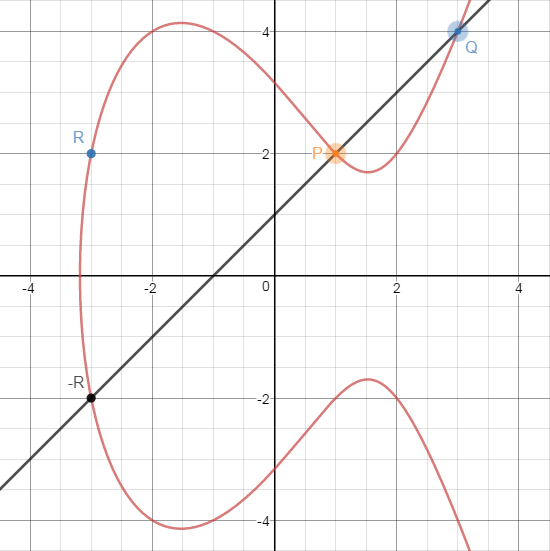
\includegraphics[width=\textwidth, left]{PQR+}
  \caption{P+Q=R}
  \label{PQR+}
 \end{minipage}
 \begin{minipage}[H]{0.5\textwidth}
  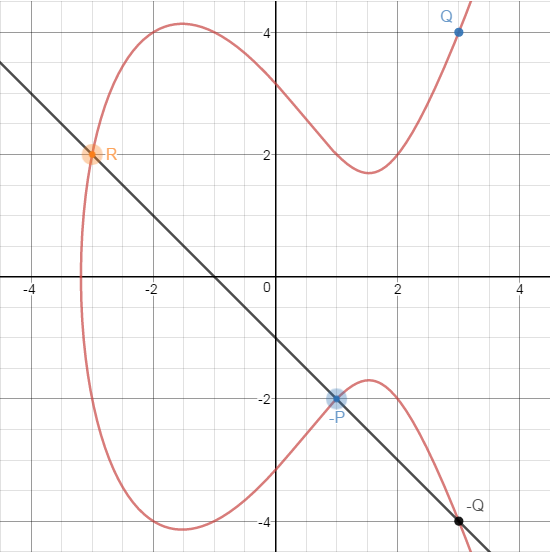
\includegraphics[width=\textwidth, right]{PQR-}
  \caption{R+(-P)=Q}
  \label{PQR-}
 \end{minipage}
 \\
 \\
\end{figure}
Illustrate le formule che governano la Legge di Gruppo, \`e bene discutere riguardo i casi particolari di questa operazione:
\begin{enumerate}
 \item Somma un punto $P$ ed il suo simmetrico $Q = -P$. 
 \\
 Tramite il metodo della Point Addition si costruisce una retta per i due punti che risulta parallela all'asse $y$ e che andr\`a ad intersecare la curva nel punto all'infinito $\mathcal{O}$. Definiamo quindi $P + Q = P+(-P) = \mathcal{O}$ (fig. \ref{PA_P+(-P)})
 \begin{figure}[H]
  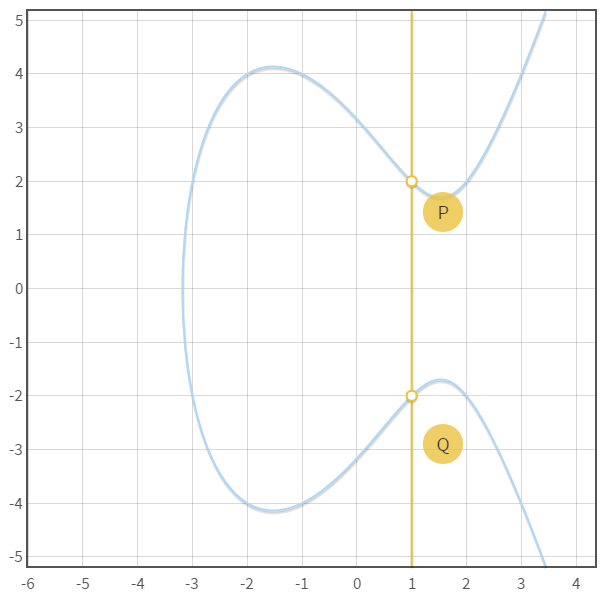
\includegraphics[width=.6\textwidth,center]{PA_P+(-P)}
  \caption{Curva $y^2 = x^3-7x+10$, $P=(1, 2)$, $Q=-P=(1, -2)$}
  \label{PA_P+(-P)}
 \end{figure}
 \label{CPsimmetrici}
 \item Somma di un punto $P$ ed il punto all'infinito $\mathcal{O}$. 
 \\ 
 La retta che unisce il punto $P$ ed il punto $\mathcal{O}$ interseca la curva in un punto 
 \\$Q = -P$. Simmetrizzando e calcolando il punto $-Q$ otteniamo il risultato ``$-(-Q) = P$".
 Ricordando che il punto $\mathcal{O}$ viene trattato come elemento identit\`a del gruppo possiamo infine scrivere $P+\mathcal{O} = \mathcal{O}+P = P$. Si consideri, a tal proposito, la stessa figura (\ref{PA_P+(-P)}) del caso precedente
 \item Somma di un punto $P$ e se stesso. 
 \\
 Non avendo due punti distinti non \`e possibile tracciare la retta per i due punti. Fissato il punto $P$, immaginiamo di prendere un secondo punto ed avvicinarlo a $P$: la retta tra i due punti diventa tangente alla curva nel punto $P$. La tangente intercetta quindi il punto $-R$ sulla curva, il punto simmetrico \`e il risultato cercato: $P + P = -(-R) = R$,
 \begin{figure}[H]
  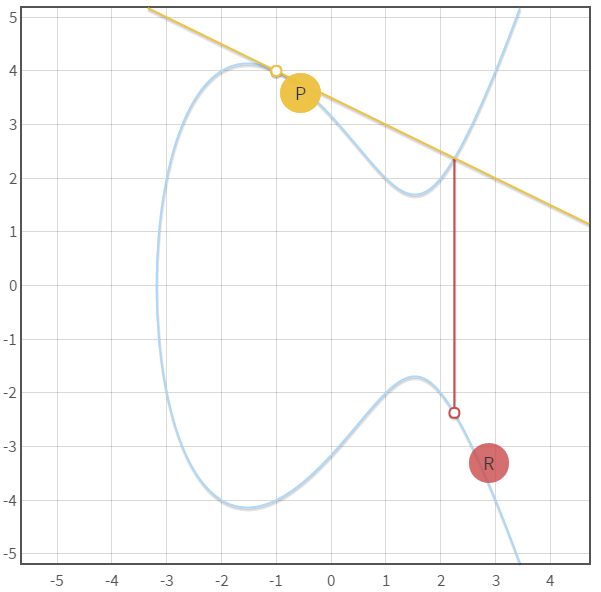
\includegraphics[width=.6\textwidth,center]{PA_P+P}
  \caption{Curva $y^2 = x^3-7x+10$, $P=Q=(-1, 4)$}
 \end{figure}
 \label{PointDoubling}
Definiamo questo caso con la dicitura ``\textit{Point Doubling}". Le equazioni viste per la Legge di Gruppo tuttavia non permettono di calcolare il punto $2P$: bisogna trovare delle formule che tengano conto della \textbf{tangente} alla curva $E$ nel punto $P$. La retta tangente $y = mx+q$ presenter\`a un coefficiente angolare $m$ dato dal gradiente dell'equazione (\ref{Forma Breve}):
\begin{align*}
E : y^2 &= x^3 + ax + b &\text{Dividiamo tutto per $y^2$}\\
1 &= \ddfrac{x^3 + ax + b}{y^2} &\text{Applichiamo il gradiente}\\
m &= \ddfrac{dy}{dx}E &\text{Imponiamo l'equazione di $E$} \\
m &= \ddfrac{dy (x^3 + ax + b)}{dx (y^2)} &\text{Che possiamo vedere come}\\
m &= \ddfrac{\ddfrac{d}{dx}(x^3 + ax + b)}{\ddfrac{d}{dy}(y^2)} &\text{Otteniamo dunque}\\
m &= \ddfrac{3x^2 + a}{2y}
\end{align*}
Si noti come il coefficiente angolare $m$ dipenda non solo dalle coordinate del punto $P$ ma anche dal coefficiente ``$a$" presente nell'equazione della curva.
\\
Definiti quindi i punti $A = (x_A, y_A)$ e $C=(x_C, y_C) = -2A$ della curva, le operazioni per effettuare una Point Doubling sono:
\begin{gather}
\begin{cases}
m = \ddfrac{3{x_A}^2 + a}{2y_A}\\
x_C = m^2 - 2x_A\\
y_C = m(x_A - x_C)-y_A
\label{point doubling 1234}
\end{cases}
\end{gather}
Le coordinate di $C$ sono calcolate mediante formule analoghe alla Point Addition: si considera l'intersezione della tangente con la curva $E$, si eguaglia il risultato al prodotto delle radici $x_A$ e $x_C$ ricordando che la prima ha molteplicit\`a 2. Infine si considerano i monomi dello stesso grado, esattamente come fatto per la Legge di Gruppo, trovando le formule qui sopra descritte
%
%
%
%
%
%
%
 \item Somma di $P+P$ quando $P$ \`e un flesso per la curva. 
 \\
 In un punto di flesso la concavit\`a della curva cambia
 %\footnote{\footnotesize{In ogni curva ellittica esistono esattamente 9 punti di flesso: 4 punti con coordinata $y$ positiva, altri 4 corrispondenti ai loro simmetrici ed, infine, il punto all'infinito.}}
 , la tangente nel punto $P$ \textbf{non} interseca nuovamente la curva, di conseguenza non intercetter\`a neanche il punto all'infinito. Il punto $P$ ha un \textbf{ordine} $n$ (formula \ref{ordineGeneratoreGruppo}), per il quale vale l'uguaglianza $nP = \mathcal{O}$. Un punto che presenti un ordine \textbf{finito} viene detto ``\textit{Punto di Torsione}" \cite{P_Torsione p9}. Essendo un punto di flesso, $P$ assume ordine 3 ed \`e quindi un punto di Torsione.
 \\
 Imponiamo $n=3$ per il nostro punto, la relazione $P+P+P = \mathcal{O}$ \`e la diretta conseguenza dell'ordine di un punto di Torsione e ci permette di scrivere: 
 \begin{center}
  $P+P=-P \iff P = flesso$
 \end{center}
 %\begin{figure}[H]  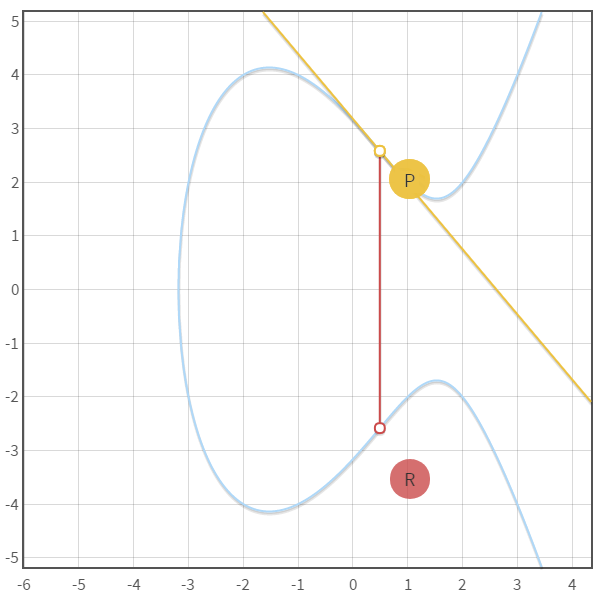
\includegraphics[width=.6\textwidth,center]{Flesso2}  \caption{Curva $y^2 = x^3-7x+10$} \begin{center} $P=Q=(0.49139, 2.58436), R=(0.49138, -2.58437)$ \\ \textit{Si \`e cercato di approssimare quanto pi\`u possibile il punto di flesso.}
\end{enumerate}
%
%
%
%
%
\section{Moltiplicazione Scalare}
Calcolare $nP$, con $n$ un numero intero, su una curva ellittica costituisce l'operazione detta ``\textit{moltiplicazione scalare}" o Point Multiplication, operazione molto comune nelle applicazioni crittografiche. Allo scopo, supponiamo di voler calcolare il punto $100P$ ed illustriamo alcune tecniche utilizzate in pratica per ottenere un risultato nel minor tempo possibile.
\\
La tecnica pi\`u intuitiva consiste nell'applicare ripetutamente la Legge di Gruppo per computare i successivi $n-1$ punti ma la scelta diventa impraticabile qualora $n$ sia un numero grande (possiamo definire tale anche un $n=100$ per motivi che verranno mostrati nei prossimi algoritmi).
\subsection{Double \& Add} 
\label{doub add}
Per introdurre questo algoritmo, ragioniamo inizialmente all'interno dei numeri naturali $\mathbb{N}$. Il nostro scopo \`e partire dal numero $m_0=1$ ed arrivare ad $m_i=100$ tramite $i$ passi e le sole operazioni di somma unitaria (detta ``\textit{Add}") e moltiplicazione con fattore 2 (detta ``\textit{Double}"):
\begin{center}
\begin{tabular}{ c | c c c }
 Passo $i$ & $m_{i-1}$ & Operazione & $m_i$\\
 \hline
 $1$ &$1$ & Double &$2$\\
 $2$ &$2$ & Add &$3$\\
 $3$ &$3$ & Double &$6$\\
 $4$ &$6$ & Double &$12$\\
 $5$ &$12$ & Double &$24$\\
 $6$ &$24$ & Add &$25$\\
 $7$ &$25$ & Double &$50$\\
 $8$ &$50$ & Double &$100$\\
\end{tabular}
\end{center}
Abbiamo raggiunto il nostro scopo in un totale di 8 passi, un risultato nettamente migliore degli $n-1=99$ passi visti precedentemente. Applicare questo algoritmo su di una curva ellittica significa nel computare una Point Addition per ogni \textit{Add} ed una Point Doubling per ogni \textit{Double}. 
\\
Parliamo allora di una possibile implementazione del metodo appena visto. Consideriamo il nostro $n = 100$ ed esprimiamolo in notazione binaria:
\begin{center}
 $n_{10} = 100_{10} \iff 1100100_2 = d_6d_5d_4d_3d_2d_1d_0 = n_2$
\end{center} 
Il procedimento da utilizzare consiste nel calcolare $n_2$ tramite l'operazione del Point Doubling per ogni $d_i$, procedendo dalla seconda cifra pi\`u significativa (in questo caso $d_5$) fino a $d_0$. Nel caso in cui troviamo ``$d_i=1$" facciamo seguire una Point Addition. 
\begin{center}
\begin{tabular}{c c l l }
 $d_i$ & Operazione & $n_2$ & Commenti\\
 \hline
  $d_6 = 1$ & / &1 & Il primo $d_i$ sar\`a sempre 1;\\
  $\mathbold{d_5 = 1}$ & Double &10 & Avendo $d_5 = 1 $ bisogna usare una ADD;\\
  & Add &1\textbf{1} & $d_5$ \`e sistemata;\\
  $d_4 = $ 0 & Double &110  \\
  $d_3 = $ 0 & Double &1100  \\
  $\mathbold{d_2 = 1}$ & Double &11000 & Come prima: segue una ADD;\\
  & Add &1100\textbf{1} & ed anche $d_2$ \`e sistemata\\
  $d_1 = $ 0 & Double &110010 \\
  $d_0 = $ 0 & Double &1100100\\
\end{tabular}
\end{center}
Questo metodo, detto \textit{Double$\&$Add}, permette il calcolo di $nP$ in $\floor{log_2(n)}+ \theta$ operazioni. Le point doubling sono $\floor{log_2(n)}$ mentre le point addition sono $\theta$, un numero corrispondente al totale di ``\emph{1}" nella notazione binaria, per cui $\theta \leq \floor{log_2(n)}$. Il costo computazionale \`e nettamente ridotto rispetto alle $n-1$ operazioni del primo metodo. 
\subsection{Montgomery Ladder}
Esiste un metodo simile alla Double$\&$Add, e viene detto \textbf{Montgomery Ladder}. Detti $P$ il punto da moltiplicare ed $n$ il moltiplicatore la cui rappresentazione binaria $n_2$ \`e ancora $d_{j}d_{j-1}\ldots d_2d_1d_0$, definiamo due parametri come $P_1=P$ e $P_2 = 2P$. La Montgomery Ladder procede come segue: \\


\begin{algorithm}[H]
\caption{Montgomery Ladder}
\begin{algorithmic}

\For{$i=j-1$ to $0$}

    \If {$d_i = 1 $}
    
        \State $P_1 =P_1+P_2$
        \State $P_2 =2P_2$
        
    \Else
    
        \State $P_2 =P_1+P_2$
        \State $P_1 =2P_1$
        
    \EndIf
\EndFor\\
\Return $P_1$
%\EndProcedure
\end{algorithmic}
\end{algorithm}
A fine ciclo, il punto cercato $nP$ \`e il valore di $P_1$.
\\
Una differenza con l'algoritmo precedente \`e il calcolo di entrambe le operazioni, una Double ed una Add, per ogni cifra $d_j$. La moltiplicazione scalare mediante la Montgomery Ladder richiede dunque $2 \floor{log_2(n)}$ operazioni. Il numero trovato corrisponde alle operazioni necessarie in una Double\&Add qualora $n=2^x-1$, $x\in \mathbb{N}$, la cui notazione binaria \`e data soli ``\emph{1}".
\\
Una riduzione del tempo computazionale \`e possibile mediante la parallelizzazione della Montgomery Ladder su due processori: uno si occuper\`a della Point Addition e l'altro della Point Doubling riuscendo a dimezzare il tempo di calcolo ed arrivare a $O(\floor{log_2(n)})$ tempo di operazioni. Lo stesso tempo computazionale viene impiegato dalla Double\&Add solo nel caso in cui la notazione binaria sia del tipo $n=2^x$, $x\in \mathbb{N}$. Si conclude che la Montgomery Ladder parallelizzata \`e generalmente pi\`u veloce della Double$\&$Add.
%
%
%
%%
%
%
%
%
%
%
%
%
\section{Campi Finiti}
Prima di iniziare a parlare di algoritmi fondati sulle curve ellittiche, \`e bene precisare che la quantit\`a \textit{finita} di memoria dei calcolatori non \`e sufficiente per gestire punti di \textit{infinite} cifre. I campi modulari $\mathbb{F}_p$ restringono le coordinate dei punti nell'intervallo $[0, p-1]$ e favoriscono l'implementazione dei concetti studiati fino ad ora. In ambito crittografico, vanno esaminate tre propriet\`a in particolare: la cardinalit\`a (o ordine) di gruppi e sottogruppi; il punto generatore del sottogruppo; il cofattore del sottogruppo.
\\
Un campo finito sul quale si intende definire una curva ellittica deve rispondere a due propriet\`a principali: il suo ordine $p$ deve essere un numero primo; la caratteristica $char(\mathbb{F}_p)$ deve essere diversa da 2 e da 3 per garantire la scrittura nella forma estesa di Tate-Weierstrass (\ref{Forma Estesa})
\begin{center}
 $\mathbb{F}_p$, $p \ne \{2, 3\}$\\
 $Y^{2} + a_1XY + a_3Y =X^3 + a_2X^2 + a_4X + a_6$ mod(p)
\end{center} 
L'equazione breve di Weierstrass (\ref{CE}) che governa la curva assume di conseguenza un carattere modulare:
\begin{gather} E(\mathbb{F}_p) =
\begin{cases}
y^2 = x^3 + ax+b \; \text{mod}(p)\\
4a^3 \ne 27b^2 \; \text{mod}(p)
\end{cases}
\bigcup \; \{\mathcal{O}\}
\label{CE mod}
\end{gather}
%
%
%
%
%
%%
%
%
%
%
%
%
\subsection{Cardinalit\`a}
\label{cardin}
Per una curva ellittica modulare non possiamo dire che la sua cardinalit\`a corrisponda all'ordine $p$: non tutti i punti del campo soddisfano l'equazione (\ref{CE mod}), a maggior ragione se consideriamo la condizione $4a^3 \ne 27b^2$ mod$(p)$ notiamo come vengano esclusi alcuni valori. Per avere un intervallo di riferimento entro il quale possa variare la cardinalit\`a $\#E$ si \`e soliti ricorrere al ``\textit{Teorema di Hasse}". Il teorema definisce $K_q$ come un campo finito avente ordine $q$ (primo, diverso da 2 e da 3), $E$ una curva ellittica definita su tale $K$. Detta $\#(E_K)$ la cardinalit\`a della curva, il valore che questa assume \`e da considerarsi nella disequazione \ref{hasse dis}:
\begin{gather}
 \#(E_K) \le (1 \pm \sqrt {q} \,)^2
 \label{hasse dis}
\end{gather}
e quindi all'interno dell'intervallo
\begin{center}
 $\ceil{q+1-2 \sqrt {q} \,} \le \#(E_K) \le \floor{q+1+2 \sqrt {q} \,}$
\end{center}
Una curva $E$ che presenti cardinalit\`a pari ad un numero primo \`e detta ``\textit{curva prima}". Se la curva presenta cardinalit\`a $\#(E_K)=q$, allora viene detta ``\textbf{anomala}". Infine, la curva viene detta ``\textbf{supersingolare}" se $\#(E_K) = q+1$ \cite{supersingolare}; alternativamente se, data la cardinalit\`a $\#(E_K) = q+1+t$, vale $t=0$ mod$(q)$ \cite{rho for poliwag}.
\\
Prendiamo dei numeri $q$ per i quali vengono rispettate le ipotesi del teorema: definita con ``min" la cardinalit\`a minima per la curva e ``max" il suo valore massimo, applicando il teorema di Hasse troviamo
\begin{center}
\begin{tabular}{ c | c c }
 q & min & max\\
 \hline
 $5$ &$2$ &$10$\\
 $19$ &$12$ &$28$\\
 $67$ &$52$ &$84$\\
 $313$ &$279$ &$349$\\
 $971$ &$910$ &$1034$\\
\end{tabular}
\end{center}
\`E importante notare che il teorema usato restituisce la cardinalit\`a della curva includendo il punto all'infinito.
\\
Un algoritmo per determinare univocamente la cardinalit\`a $\#E$ \`e quello di Schoof. Per prima cosa chiamiamo $N \geq 4\sqrt{q}$ un numero la cui scomposizione in fattori primi corrisponda a $N=\prod_{i=1}^j p_i $. Successivamente, per ogni fattore $p_j$ viene calcolato un parametro $t_{p_j}$ come descritto in \cite{schoof}. Infine, il calcolo di $\#E$ viene reso possibile dal Teorema Cinese del Resto (descritto nel capitolo \ref{poliwag}) applicato al sistema seguente:
\begin{center}$
\begin{cases}
    \#E = 1+q-t_{p_1} \text{ mod}(p_1)\\
    \#E = 1+q-t_{p_2} \text{ mod}(p_2)\\
    \ldots \\
    \#E = 1+q-t_{p_j} \text{ mod}(p_j)\\
\end{cases}$
\end{center}
%
%
%
%\begin{figure}[H] \includegraphics[width=.9\textwidth,center]{EC_mod(p)} \caption{Curva $y^2 = x^3-7x+10$ mod $(p)$, $p = \{19, 97, 127, 487\}$} \end{figure}
%\begin{figure}[H]  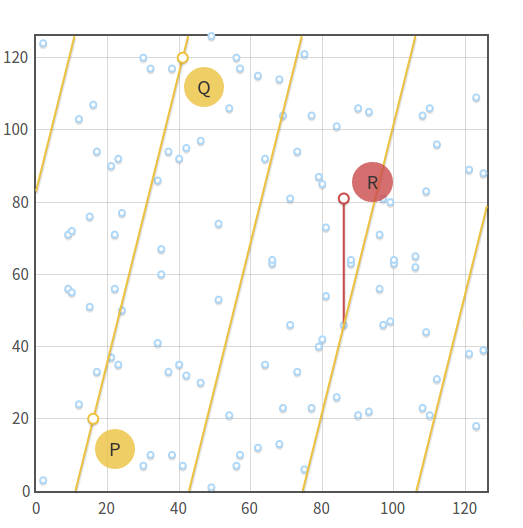
\includegraphics[width=.7\textwidth,center]{ECmodPA}  \caption{Curva $y^2=x^3+2x+3$ mod$(19)$}  \begin{center}  $P = (3, 13)$, $Q=(10, 15)$, $R = -(P+Q) = (15, 8)$\\   Cardinalit\`a della curva: 20 elementi  \end{center}   \label{ECmodPA} \end{figure}
%
%
%
%
%
%
\subsection{Punti Generatori}
Un punto $P$ che generi un gruppo ciclico viene detto Generatore del gruppo. Tutti i punti appartenenti a questo gruppo possono esser calcolati applicando ripetitivamente la Legge di Gruppo al punto $P$. 
\\
Prendiamo la curva $E: y^2 = x^3 +2x +2$ mod$(17)$ ed il punto $P = (5, 1)$. La curva ed il sottogruppo generato da $A$ contengono entrambi 19 elementi in totale. L'elemento successivo possiamo dirlo $Q=2P$ e si calcola con le stesse formule della Point Doubling (formule \ref{point doubling 1234}) espresse in modulo 17 per il caso in esame.
\begin{figure}[H] 
    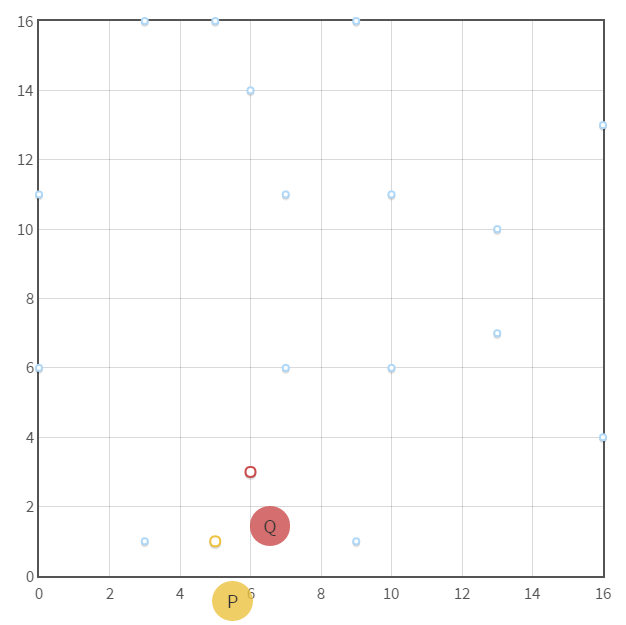
\includegraphics[scale=0.5, center]{PD_mod(17)} 
    \caption{Curva $y^2=x^3+2x+2$ mod$(17)$, punto $P = (5, 1)$, $Q=2P = (6, 3)$} 
\end{figure} 
Si noti che ora \textbf{l'asse di simmetria} non risulta pi\`u essere $y=0$ ma \textbf{diventa} $\mathbold{y=p\big / 2}$ eccezion fatta per i punti che giacciono sull'asse $x$. Questi punti, descritti con le notazioni equivalenti tra loro $(x, y)=(x, 0)$ mod$(y)$, risultano simmetrici a loro stessi essendo vero che $y=0$ mod$(y)$.
\\
\`E possibile fare un'ulteriore verifica del risultato contando i punti tramite una serie di Point Addition: partiamo dal punto $A=(5, 1)$ identifichiamo le coordinate di $nA$ con $(nA_x, nA_y)$ 
\begin{center}
\begin{tabular}{ r r l | r r l}
 $n$ & $nA_x$ & $nA_y$ & $n$ & $nA_x$ & $nA_y$\\
 \hline
 $1$ & 5 & 1 & $10$ & 7 & 11 \\
 $2$ & 6 & 3 & $11$ & 13 & 10\\
 $3$ & 10 & 6 & $12$ & 0 & 11\\
 $4$ & 3 & 1 & $13$ & 16 & 4\\
 $5$ & 9 & 16 & $14$ & 9 & 1\\
 $6$ & 16 & 13 & $15$ & 3 & 16\\
 $7$ & 0 & 6 & $16$ & 10 & 11\\
 $8$ & 13 & 7 & $17$ & 6 & 14\\
 $9$ & 7 & 6 & $18$ & 5 & 16\\
 & & & $19$ & / & /
\end{tabular}
\end{center}
Il punto $19A$ rappresenta il punto all'infinito e verifica che la cardinalit\`a della curva $E$ sul campo $\mathbb{F}_{17}$ \`e 19. Trovandoci in un campo modulare, il punto $20A$ esiste e corrisponde alla Point Addition di $19A+A=\mathcal{O}+A = A$. In generale possiamo scrivere ogni punto $kP$ basandoci sulla seguente espressione:
\begin{gather}
[k \text{ mod} (\#E_K)] \cdot P
\label{punti modulari}
\end{gather}
Come anticipato nel ``Caso Particolare (\ref{CPsimmetrici})" abbiamo $A+18A = 19A = \mathcal{O}$ poich\`e si applica la Legge di Gruppo a due punti distinti di eguale ascissa ($x_A=x_{18A}=5$) ma ordinata diversa ($y_A=1$, $y_{18A}=16$). Sebbene tale caso presupponesse che i due punti sommati dovessero essere simmetrici tra loro, ora la simmetria sembra venir meno. Ricordando che l'asse di simmetria \`e $y= p \big / 2 = 17 \big / 2 = 8.5$ possiamo facilmente verificare che i due punti rispettino effettivamente la simmetria. Possiamo, ad esempio, sommare le ordinate dei due punti e dividere per due, ottenendo il punto medio tra $A$ e $18A$:
\begin{center}
 $\ddfrac{y_A+y_{18A}}{2}=\ddfrac{1+16}{2}=\ddfrac{17}{2}=8.5$
\end{center}
confermando che il punto medio tra $A$ e $18A$ si trova sull'asse di simmetria e quindi verifica quanto affermato prima. 
\\
Restando vero che per ogni punto della curva esiste il suo simmetrico, possiamo evidenziare un risultato importante:
\begin{center}
 $2A + 17A = 3A + 16A = 4A + 15A = \ldots = 19A = \mathcal{O}$
\end{center}
Ognuna di queste coppie di punti presenta ascissa uguale ed ordinata diversa, sono tutte coppie di punti simmetrici tra loro. Si arriva allora alle seguenti \textit{Considerazioni Personali}:
\begin{enumerate}
 \item Il calcolo dei 19 punti ha mostrato una ricorsivit\`a 
nei valori delle \textbf{ascisse}: i primi 9 punti hanno ascissa nella sequenza $5, 6, 10, 3, 9, 16, 0, 13, 7$ mentre i successivi 9 hanno ascissa in sequenza invertita. Inoltre solo due punti \textit{successivi tra loro} presentano la stessa ascissa: $9A$ e $10A$, punti simmetrici, la cui somma \`e $19A = \mathcal{O}$. Si \`e cercato quindi di ideare un metodo efficace per determinare la cardinalit\`a delle curve in campi modulari arrivando ad affermare quanto segue:
\\
``Dati due punti $nG$ e $(n+1)G$ di una curva $E$ definita su un campo finito $K_q$, detto $H$ il sottogruppo generato dal punto $G$, se vale $x_n = x_{n+1}$ allora le seguenti affermazioni
\begin{equation}
\begin{cases}
 nG + (n+1)G = \mathcal{O}\\
 \#H = n+(n+1) = 2n+1
\end{cases}
 \label{CPcard_dispari}
\end{equation}
 sono vere e la cardinalit\`a \`e sempre \textbf{dispari}. \`E possibile generalizzare la (\ref{CPcard_dispari}) per ogni coppia di punti $(n-k)G$ e $(n+1+k)G$ aventi ascisse uguali $x_{n-k} = x_{n+k+1}$. La distanza, in termini di successive Point Addition tra i due punti, \`e pari a $2k+1$. Alcuni esempi di quanto affermato sono dati dalle seguenti relazioni: $(2A + 17A)=(3A + 16A)=(4A + 15A)=\mathcal{O}$.
 \\
 \\
 Se invece si trova che, dati due punti $(n-1)G$ ed $(n+1)G$, le loro ascisse coincidano $x_{n-1} = x_{n+1}$, allora la (\ref{CPcard_dispari}) diventa
 \begin{equation}
\begin{cases}
 2nG = \mathcal{O}\\
 \#H =2n
\end{cases}
 \label{CPcard_pari}
\end{equation}
in questo caso abbiamo sempre cardinalit\`a \textbf{pari}. Anche in questo caso evidenziamo una generalizzazione: la (\ref{CPcard_pari}) vale per ogni coppia di punti $(n-k)G$ e $(n+k)G$ di medesima coordinata $x_{n-k} = x_{n+k}$. La distanza tra i due punti corrisponde a calcolare $2k$ Point Addition".
 \\
 \\
 Possiamo verificare che quanto espresso valga solo all'interno di sottogruppi del campo $K_p$ servendoci di un esempio: data la curva $E : y^2 = x^3 + 4x+5$ nel campo $\mathbb{Z}/31\mathbb{Z}$ e punto generatore $P = (18,9)$. Dal teorema di Hasse la curva ha cardinalit\`a compresa nell'intervallo $[27, 37]$ ed il conto esatto mostra che $\#E_K= 28$. Il punto $P$ considerato genera un sottogruppo $H$ i cui punti sono $P=(18,9), 2P=(0,6)$, $3P=(7,29)$, $4P=(7,2)$, $5P=(0,25)$, $6P=(18,22)$, $7P= \mathcal{O}$. La ricorsivit\`a delle ascisse vista precedentemente si mantiene valida in $H$, deduciamo che la cardinalit\`a di questo sottogruppo \`e 7 e resta valida la relazione 
 \begin{center}
  $3P+4P = \mathcal{O} \Rightarrow \#H = 7$
 \end{center} in quanto $3P$ e $4P$ sono punti successivi tra loro ed ascissa $x_{3P} = x_{4P} = 7$. In aggiunta, restano valide le uguaglianze $P+6P=2P+5P = \mathcal{O}$. Infine considerando che $\#H \ne \#E_K$ si dimostra che l'affermazione precedente resta valida all'interno di sottogruppi $H \subset K_p$. 
 %
 %
 %
 \item In un sottogruppo, possiamo calcolare il punto simmetrico di $Q = (x_Q, y_Q)$ considerando ``$-Q = (x_Q, \#H-y_Q)$", dove $\#H$ \`e cardinalit\`a del sottogruppo $H \subset \mathbb{F}_{31}$ visto nell'esempio precedente. Utilizzando i punti $Q$ e $-Q$, cerchiamo di determinare $\#H$.
 \\
 La Legge di Gruppo ci permette di dire che $Q-Q = \mathcal{O} = \#H \cdot G$ in quanto simmetrici ed appartenenti ad un campo modulare. Dette $n$ e $m$ le loro molteplicit\`a tali per cui $Q = nG$ e $-Q = mG$, la considerazione precedente ci porta ad affermare che $n+m = \#H$. La conclusione alla quale arriviamo \`e che, per due numeri naturali $n$ ed $m$
 \begin{gather}
  n, m \in \{0, 1, \ldots, q-1\} \mid Q = nG, -Q = mG \Rightarrow \#H = n+m
  \label{Cons Pers 2}
 \end{gather}
 Siamo quindi riusciti a determinare la cardinalit\`a di $H$ a partire da due punti simmetrici tra loro.
\end{enumerate}
%
%
%%
%
%
%
%
%
%
%
%
%
\subsection{Cofattore}
Riprendiamo il concetto di cofattore di un sottogruppo. Come detto nel capitolo (\ref{base gruppi}), sulla base del teorema di Lagrange possiamo affermare che dato un gruppo $G$ con cardinalit\`a $\#G$, il suo sottogruppo $H$ avr\`a cardinalit\`a detta $\#H$ tale che valga la seguente formula:
\begin{center}
 $h = \ddfrac{\#G}{\#H}$, $h \in \mathbb{Z}$
\end{center}
Dove con $h$ si esprime il cofattore di $H$.
\\
Possiamo far uso del cofattore per determinare la cardinalit\`a di un sottogruppo partendo dalla sola $\#G$. Prendiamo in esempio la curva $E : y^2 = x^3+4x+5$ nel campo $\mathbb{F}_{31}$. La curva presenta cardinalit\`a $\#G=28$ i cui divisori interi sono $T = \{1, 2, 4, 7, 14, 28\}$. A questo punto dobbiamo introdurre un generatore: preso il punto $P=(18, 9)$ cerchiamo di ottenere il punto $\mathcal{O}$ mediante successive Point Multiplication $tP$ dove $t \in T$ \`e il generico elemento di $T$. Troviamo che $7P = 14P=28P= \mathcal{O}$ e la relazione (\ref{punti modulari}) non \`e pi\`u valida nel sottogruppo poich\`e viene verificata per pi\`u di un valore. Possiamo esporre tale formula in modo pi\`u generale dicendo che \begin{gather}
[k \text{ mod} (\#H)] \cdot P
\end{gather}
In questa ottica affermiamo che $\#H=7$ per la curva in considerazione per via del fatto che $t_5=14$, $t_6=28$ sono multipli interi di $\#H$: per la ciclicit\`a dell'algebra modulare questi valori corrispondono allo stesso elemento in modulo 7. Di conseguenza il sottogruppo $H$ presenter\`a cofattore $h = \#G/\#H=28/7 = 4$. 
\\
Inoltre solo il pi\`u grande divisore primo $t$ rappresenta la cardinalit\`a del sottogruppo.
\\
Una curva come $E: y^2 = x^3 +2x+4$ mod$(13)$ presenta cardinalit\`a $N=17$ e, per ogni suo punto, viene generato un sottogruppo $H$ di ancora 17 elementi. Essendo vero che i divisori di $N$ sono solo $1$ e se stesso si conclude che, preso un qualsiasi punto della curva che non sia $\mathcal{O}$, esister\`a un sottogruppo $H$ di cardinalit\`a $\#H = 17$. Per la conclusione proposta si \`e dovuto escludere il divisore ``\emph{1}" per il seguente motivo: preso un punto $P$, generatore del sottogruppo $H$, sappiamo che bisogna rispettare la relazione $\#H \cdot P = \mathcal{O}$; se avessimo assunto $\#H = 1$ avremmo ottenuto
\begin{center}
 $\#H \cdot P = 1P = P = \mathcal{O}$
\end{center}
identificando quindi un sottogruppo avente il solo elemento neutro della Legge di Gruppo e nessun altro punto.
\\
Sulla base di quanto detto finora possiamo concludere che i sottogruppi $H$ presentano cofattore $h=1$ qualora tale sottogruppo comprenda tutti (e soli) i punti della curva.

%
%
%
%
%
%
%
%
%
%
%
%
%
%
%
%
%
%
%
%
%
%
%
\chapter{Algoritmi per la Sicurezza Informatica}
\label{ecc algo}
Consideriamo in questo capitolo alcuni algoritmi della sicurezza informatica ed i loro corrispondenti algoritmi basati sugli studi effettuati. Tratteremo di: crittografia simmetrica, asimmetrica e firma digitale.
\\
Riguardo la crittografia simmetrica verr\`a mostrato il paradigma ElGamal per cifrare in modo sicuro un messaggio, seguito poi dalla sua variante per mezzo delle curve ellittiche, la \textit{Crittografia Ellittica Simmetrica}. Proseguiremo con la crittografia asimmetrica illustrando il funzionamento del protocollo RSA, evidenziandone (qui e nei capitoli successivi) i motivi che spingono ad approcciarsi verso nuovi algoritmi, e quindi il corrispettivo protocollo: ECDH. Infine tratteremo della firma digitale implementata negli algoritmi DSA e ECDSA.
%
%
%
%
%
%
%
%
%
%
%
%
\section{ElGamal}
La crittografia di un messaggio tramite l'algoritmo di ElGamal si basa sulla generazione di parametri pubblici e privati \cite{guide to ECC}. Identifichiamo i parametri pubblici con la notazione $t = (p, q, g, K^+)$, la scelta di questi avviene nel seguente modo:
\begin{enumerate}
 \item \textbf{p} deve essere un numero primo. Si preferiscono numeri molto grandi in modo da garantire la sicurezza dell'algoritmo, tuttavia ci\`o comporta un maggior impiego di risorse per i calcoli;
 \item \textbf{q} deve essere un divisore primo di ``$p-\emph{1}$";
 \item \textbf{g} deve corrispondere ad un numero scelto nell'intervallo $[1, p-1]$ avente ordine pari a $q$.
\end{enumerate}
Possiamo quindi definire la chiave privata $K^-$ come un numero intero, casuale, scelto nell'intervallo $[1, q-1]$. Complementare ad essa, calcoliamo la chiave pubblica come $K^+ = g^{K^-}$ mod$(p)$.
\\
Riuscire a trovare $K^-$ a partire dai parametri pubblici costituisce il ``\textit{Problema del Logaritmo Discreto}". Verr\`a fatto riferimento al problema appena descritto mediante la notazione DLP, dall'inglese ``\textbf{D}iscrete \textbf{L}ogarithm \textbf{P}roblem". 
\\
\\
Ci interessiamo ora ad esporre come funzioni la crittografia di un messaggio $m$. L'utente Alice, intenzionata all'invio sicuro del suo $m_A$, si comporta come segue:
\begin{enumerate}
 \item Sceglie un numero casuale $k$ appartenente all'intervallo $[1, q-1]$;
 \item Calcola $c_1 = g^k$ mod$(p)$;
 \item Calcola $c_2 = m \cdot (K^+)^k$ mod$(p)$;
 \item Invia la coppia $(c_1, c_2)$ al suo interlocutore Bob. 
\end{enumerate}
Bob \`e capace di decifrare il messaggio procedendo al calcolo:
\begin{align*}
c_2 \cdot c_1^{-K^-} \text{ mod}(p) &=\\
 &= m \cdot (K^+)^k \cdot g^{k  (-K^-)} \text{ mod}(p)\\
 &= m \cdot g^{k  (K^-)} \cdot g^{-k (K^-)} \text{ mod}(p)\\
 &=m
\end{align*}
In questo modo si \`e recuperato il messaggio originale, tuttavia sia per Alice che per Bob \`e necessario conoscere la chiave privata $K^-$ implicando una precedente comunicazione nella quale \`e avvenuto lo scambio della chiave simmetrica, il segreto condiviso.
%
%
%
%
%
%
%
%
\section{Crittografia Ellittica Simmetrica}
La variante ellittica di ElGamal prevede un maggior numero di parametri pubblici. In questo caso bisogna pensare dapprima all'accordo (ed alla generazione) di una curva ellittica sulla quale operare. Campo, cardinalit\`a, generatore e cofattore sono quindi ulteriori elementi di cui necessiteremo:
\begin{itemize}
 \item i numeri \textbf{a}, \textbf{b} che serviranno da coefficienti nell'equazione (\ref{CE mod}) per descrivere la curva ellittica;
 
 \item un numero primo \textbf{p} atto a specificare la cardinalit\`a del campo $\mathbb{F}p$;
 
 \item il punto \textbf{G}, generatore del sottogruppo $H$;
 
 \item il numero primo \textbf{n = $\#H$}, rappresentante la cardinalit\`a del sottogruppo;
 
 \item il numero \textbf{h}, ovvero il cofattore.
\end{itemize}
Per semplicit\`a andiamo ad identificare tutti questi valori sotto il nome di $t$; la sua espressione \`e quindi:
\begin{center}
 $t= (a, b, p, G, n, h)$
\end{center}
\subsection{Codificare il Messaggio}
\label{codifica}
Codificare, inviare e decodificare un messaggio di testo in termini di curve ellittiche \`e un problema leggermente pi\`u complesso rispetto ad altri algoritmi. ElGamal, e similmente qualsiasi altro algoritmo che preveda la cifratura di un messaggio di testo, divide il messaggio in blocchi a lunghezza fissa di $B$ bit. Eventualmente una parte dei bit finali viene posta a 0 in modo da ottenere un completamento a $B$ bit favorendo una corretta codifica per messaggi di lunghezza arbitraria. Ogni parola di $B$ bit viene quindi criptata secondo le specifiche dell'algoritmo, inviata al destinatario ed infine decriptata. Il messaggio originale \`e dato dalla concatenazione di tutte queste parole decriptate.
\\
Quanto avviene per le curve ellittiche \`e differente: abbiamo bisogno di rappresentare un messaggio di testo in punti sulla curva. Dobbiamo assicurarci che ogni simbolo abbia una corretta rappresentazione, individuata da un punto $K$-razionale. Aggiungiamo il fatto che cambiare i coefficienti $a$, $b$ della curva oppure la cardinalit\`a $p$ del campo $\mathbb{F}_p$ identifica una nuova, diversa, curva e di conseguenza una differente rappresentazione per ciascun carattere del messaggio. \textit{Ogni curva porta a diverse rappresentazioni dello stesso messaggio}.
\\
Assumiamo di voler codificare il nostro messaggio velocemente e semplicemente facendo uso di un algoritmo probabilistico \cite{codifica messaggi su CE}. La prima cosa di cui dobbiamo assicurarci \`e che la probabilit\`a $P$ di fallire nella codifica sia molto bassa; a tale scopo definiamo un numero $k$ come $2^{-k} < P$. Valori concreti per questo parametro possono esser scelti nell'intervallo $[30, 50]$.
\\
Scegliamo di codificare i caratteri del testo in chiaro (lettere, numeri e/o simboli) nella forma di numeri interi. Possiamo, ad esempio, codificare un testo in cui vengono permessi solo i caratteri $A, B, \ldots, Z$ mappandoli sui numeri interi $1, 2, \ldots, 26$, per un totale di $T$ caratteri codificati. Inoltre dobbiamo permettere che ogni carattere possa esser rappresentato come un punto distinto dagli altri sulla curva: la cardinalit\`a $p$ del campo diviene di fondamentale importanza per gestire messaggi con molti caratteri diversi. Per permettere un tale requisito dobbiamo assicurarci quindi che valga la relazione $p > Tk$. Gli ultimi due parametri da definire sono: $c$ ovvero il valore numerico che rappresenta il nostro carattere; $j$ un numero compreso nell'intervallo $j \in [1, k]$. L'algoritmo di codifica consiste quindi nel considerare dapprima $j=1$ e calcolare
\begin{center}
$\begin{cases}
 x = ck + j \text{ mod}(p)\\
 y^2 = x^3 + ax + b \text{ mod}(p)
 \end{cases}$
\end{center}
In caso la $y$ trovata non corrispondesse ad un numero $K$-razionale, si procede ad incrementare la $j$ di 1 e si calcolano di nuovo le coordinate $x$, $y$. Il fallimento dell'algoritmo consiste nel non poter trovare un valore di $y$ accettabile per nessun valore di $j$.
\\
Se la codifica \`e andata a buon fine allora $c \iff P=(x, y)$ con le coordinate appena calcolate. Iterare l'algoritmo per ogni carattere del messaggio permette di codificarne l'intero contenuto in una serie di punti. 
\\
\\
Assunto che siamo riusciti a codificare correttamente il carattere $c$, passiamo a trattare della sua corretta decodifica. Otteniamo il carattere iniziale applicando la seguente formula:
\begin{center}
 $c = \Big \lfloor \ddfrac{x-1}{k} \Big \rfloor$
\end{center}
Qui intendiamo il carattere $c$ come la sola parte intera del risultato, per questo si \`e evidenziata l'operazione di arrotondamento per difetto $\lfloor \cdot \rfloor$.
%
%
%
%
%
%
%
\subsubsection{Codifica proposta}
%\textbf{Nota}: \textit{Questa intera sezione si basa interamente su considerazioni personali e mira a descrivere un algoritmo funzionante e deterministico per la codifica di messaggi tramite le curve ellittiche}.\\\\
Codificare e decodificare un messaggio $m$ devono essere due funzioni facilmente computabili ed eseguibili in modo deterministico per entrambi Alice e Bob. L'idea che si propone per soddisfare tali richieste si basa sulle seguenti considerazioni:
\begin{enumerate}
 \item Ogni carattere ammesso $C$ nella codifica viene reso nel suo corrispondente valore decimale $c$ in ASCII secondo quanto riportato in \cite{ascii}
 \item Ipotizzando di accettare $x$ caratteri diversi tra loro, la curva $E$ dovr\`a presentare una cardinalit\`a minima di $n = x + y$. Il numero $y$ corrisponde alla somma dei punti minimi necessari per determinare ogni punto sulla curva in modo unico. Punti di cui tener conto sono: il punto all'infinito $\mathcal{O}$; $K^S$ che serve da chiave simmetrica qualora la codifica avvenga tramite crittografia simmetrica; $K^+$ che serve da chiave pubblica qualora si utilizzi una crittografia asimmetrica; $S$ detto Seed, un punto casuale per mezzo del quale possiamo aggiungere entropia negli algoritmi ellittici, introdotto pi\`u avanti
 \item Dai parametri pubblici $t$ prendiamo $G$, il punto generatore. La codifica consiste nel far corrispondere ogni carattere al suo corrispondente punto $cG$ della curva
 \label{Pcodifica}
\end{enumerate}
La decodifica consistere nell'avere una tabella di due colonne in cui si riportano il valore ASCII del carattere $c$ e l'ascissa del punto $cG$; vedasi a tal proposito la tabella seguente
\begin{center}
\begin{tabular}{ c c }
 Carattere $\to$ c & cG\\
 \hline
 @ $\to$ 64 & $x_{64}$\\
 A $\to$ 65 & $x_{65}$\\
 a $\to$ 97 & $x_{97}$\\
 7 $\to$ 55 & $x_{55}$\\
 . $\to$ 46 & $x_{46}$
 \label{decodifica1}
\end{tabular}
\end{center}
La colonna ``cG" tiene conto solo della coordinata $x_c$ del punto $cG=(x_c, y_c)$ in modo da diminuire la memoria necessaria al mantenimento della tabella. Possiamo dimezzare i record da memorizzare se ad ogni coordinata $x_c$ facciamo corrispondere due caratteri consecutivi della tabella ASCII. Indichiamo i due caratteri ``@" e ``A" con la stessa ascissa $x_c$. Al carattere con codice $c$ \textbf{pari} facciamo corrispondere l'ordinata $y_c$ positiva, al carattere con codice \textbf{dispari} facciamo corrispondere la $y_c$ negativa. Procedendo in modo simile per tutti i caratteri da rappresentare arriviamo ad ottenere una tabella simile:
\begin{center}
\begin{tabular}{ c c }
 Caratteri $\to$ c & cG\\
 \hline
 (@, A) $\to$ 64 & $x_{64}$\\
 (b, c) $\to$ 98 & $x_{98}$\\
 (0, 1) $\to$ 48 & $x_{48}$\\
 (6, 7) $\to$ 54 & $x_{54}$\\
 (., /) $\to$ 46 & $x_{46}$
 \label{decodifica2}
\end{tabular}
\end{center}
Esempio: Alice sta codificando un messaggio da mandare a Bob e si trova a codificare il carattere ``\emph{1}". Il suo valore ASCII \`e 49: decrementa quindi il codice a $c=48$ e computa $cG=48G$. Il carattere da inviare deve considerare l'ordinata $y_{48}<0$ quindi Alice simmetrizza il punto \textit{se necessario} ed infine invia il punto $cG$ con ordinata negativa a Bob. Quest'ultimo cercher\`a la coordinata $x_{48}$ nella tabella trovando il valore $c=48$. Guardando il segno di $y_{48}$ Bob deduce che il carattere effettivo non \`e 48 ma il successivo ovvero $c=49$ dal quale ottiene correttamente ``\emph{1}".
\\
\\
Pseudocodici per l'implementazione.
\\
Input codifica: carattere $C$, punto $G$ della curva (preso dai parametri $t$),
\begin{algorithm}[H]
\caption{Codifica}
\begin{algorithmic}
%\Procedure{Codifica}{}
\State $\textit{c} \gets \text{ASCII2DEC}\textit{(C)}$ \Comment{Converte $C$ in intero}
\State $is\_odd \gets \textit{c\%2}$
\If {$is\_odd$} 
\State $c \gets c-1$ \Comment{Se $c$ \`e dispari, viene diminuito di 1}
\EndIf
\State $Q \gets cG$
\If {$((y_Q > 0$ and $is\_odd)$ or $(y_Q < 0$ and $!is\_odd))$} 

\Return -Q
\EndIf\\
\Return Q
%\EndProcedure
\end{algorithmic}
\end{algorithm}
%
%
%
%
%
%
Con la notazione ``$!is\_odd$" si fa riferimento alla negazione di ``$is\_odd$" ossia si sta identificando un carattere con codice ASCII pari.
\\
\\
Passiamo ora a mostrare la decodifica del punto.
\\
Input decodifica: il punto $Q = (x_Q, y_Q)$ inviato da Alice
\begin{algorithm}[H]
\caption{Decodifica}
\begin{algorithmic}
\State $d \gets Decode\_Table(x_Q)$ \Comment{Prende il valore ASCII di $x_Q$ dalla tabella}
\If {$y_Q<0$} 
\State $d \gets d+1$
\EndIf\\
\Return DEC2ASCII(d) \Comment{Ritorna il carattere ASCII corrispondente}
\end{algorithmic}
\end{algorithm}
Infine \`e possibile aggiungere casualit\`a agli algoritmi visti facendo uso di un segreto condiviso tra le due parti ma oscuro a tutti gli altri utenti della rete: la chiave simmetrica $K^S=(x_S, y_S)$. Essendo anch'essa un punto della curva, definiamo la funzione ``\textit{shuffle}$(x_S, y_S, n)$" che ne usa le coordinate per dare in output un numero $s$ modulo $n$. Alice e Bob possono computare quindi $(s+c)G$ per codificare in modo unico i caratteri ASCII e generare la loro tabella $(s+c) \to (s+c)G$. Lo pseudocodice per la codifica cambia leggermente: si dovr\`a ora calcolare il punto $Q \gets (c\mathbold{+s})G$ invece che $Q \gets cG$.
%
%
%
%
%
%
%
%
%
%
%
%
\subsection{Inviare il Messaggio}
\label{Crittografia Ellittica}
Si evidenzia adesso come avviene l'invio in modo sicuro di un messaggio da parte di Alice. Assumiamo che, detto $m$ il messaggio, $m_i$ sia il suo carattere $i$-esimo da codificare. Facendo uso dei parametri pubblici $t = (a, b, p, G, n, h)$ \`e possibile agire come segue:
\begin{enumerate}
 \item Il primo passo che compie Alice \`e prendere $m_i$ e rappresentarlo come punto $M$ della curva
 \item Scegliamo la chiave privata $d$ come un numero intero appartenente all'intervallo $[1, n-1]$
 \item Calcoliamo la chiave pubblica come $P = dG$; questa funziona da chiave simmetrica per i due interlocutori
 \item Calcoliamo infine il messaggio cifrato $C = M + dP$
 \item Si invia all'interlocutore Bob la coppia $(P, C)$
\end{enumerate}
Bob \`e in grado di decifrare il messaggio trovando dapprima $M= C-dP$ ed infine estraendo il messaggio $m$ dal punto $M$ tramite un algoritmo di decodifica.
\\
Verifichiamo il corretto funzionamento dell'algoritmo: sappiamo che il messaggio crittografato \`e $C = M + dP$ e che $P = dG$; il coefficiente $d$ \`e analogo alla chiave simmetrica di ElGamal. Essendo vero che tale chiave simmetrica $P$ \`e conosciuta da entrambi gli interlocutori e loro solamente, Bob (come anche Alice) sar\`a in grado di calcolare il punto $dP$ usando l'algoritmo della Double\&Add o la Montgomery Ladder. L'ultimo passo da compiere \`e applicare la Legge di Gruppo tra il punto $C$ ed il punto $S = -dP$ ottenendo \begin{center}
$C+S = C-dP = (M+dP) - dP = M$
\end{center}
Bob riesce infine a calcolare il punto $M$ ed ha la possibilit\`a di decodificarlo nel carattere $m_i$.
\\
Per questo algoritmo, parliamo di ECDLP riferendoci al problema di calcolare la chiave privata $d$ a partire dall'equazione $Q = dP$. La sigla ECDLP, intesa come \textbf{E}lliptic \textbf{C}urve \textbf{D}iscrete \textbf{L}ogarithm \textbf{P}roblem, \`e data per analogia al problema visto con ElGamal. Inoltre, sebbene le curve ellittiche non presentino calcoli esponenziali o logaritmici, la sigla mira ad evidenziare la difficolt\`a computazionale del problema. Risolvere l'ECDLP si ritiene essere un compito ben pi\`u oneroso del DLP come verr\`a mostrato nel capitolo \ref{ecdlp}.
%
%
%
%
%
%
%
%
%
%
%
%
%
\section{RSA}
Il sistema a chiave asimmetrica (o pubblica) pi\`u noto e diffuso \`e RSA, utilizzato per autenticare utenti sulla rete e per garantire integrit\`a dell'informazione. L'algoritmo si propone di garantire la protezione della comunicazione tra due interlocutori Alice e Bob facendo uso di due chiavi, una privata $K^-$ ed una pubblica $K^+$. La matematica alla base di RSA \`e data dal \textit{Teorema di Eulero} secondo il quale ``se due numeri $a$ e $n$ sono coprimi allora $a^{\theta(n)} = 1$ mod$(n)$". La funzione $\theta(n)$ di Eulero corrisponde al totale di numeri interi, positivi, minori di $z$ e coprimi (\emph{senza alcun fattore in comune}) ad esso. Due esempi: $\theta(10) = 4$, ovvero $\{1, 3, 7, 9\}$;  preso invece un numero primo $\theta(11) = 10$. Per ogni numero primo $z$ risulta chiaro che la sua funzione $\theta$ corrisponda a $z-1$. 
\\
Una propriet\`a importante di questo teorema \cite{libro 900 pagine} \`e che, dati due numeri primi $p$ e $q$, il loro prodotto \`e $n=pq$ per il quale possiamo scrivere:
\begin{center}
    $\theta (n) = \theta (pq) = \theta (p) \cdot \theta (q) = (p-1)(q-1)$
\end{center}
Adesso \`e possibile esporre come vengano generate le chiavi crittografiche secondo l'algoritmo RSA:
\begin{enumerate}
 \item Si scelgono due numeri casuali $p$ e $q$. Per un corretto funzionamento dell'algoritmo bisogna assicurarsi che i due numeri siano entrambi \textbf{primi} e di \textbf{ordine simile} ma \textit{lunghezza in bit differente} in modo da rendere la fattorizzazione pi\`u difficile \cite{RSAp+q};
 \item Si calcola $n=p \cdot q$. Tale numero verr\`a detto \textbf{modulo} per le chiavi privata e pubblica, inoltre la lunghezza in bit di $n$ corrisponde alla \textit{lunghezza della chiave} usata per l'algoritmo;
 \item Si calcola $\theta(n) = (p-1)\cdot (q-1)$; la formula \`e corretta se pensiamo che entrambi $p$, $q$ siano numeri primi. Questo valore appena calcolato va mantenuto segreto;
 \item Va ora scelto un numero $e_A$ tale che $ 1<e_A<n$, coprimo a $\theta(n)$;
 \item Infine va scelto un numero $d_A$ tale che ``$e_Ad_A-1$" sia interamente divisibile per $\theta(n)$, ovvero $e_Ad_A= 1$ mod$(\theta(n)) $. Rispettare tale uguaglianza permette di dire che il numero $e_Ad_A -1$ \`e sempre un multiplo intero di $\theta(n)$ e quindi, pi\`u in generale, vale ``$e_Ad_A = 1 + h\theta(n) $ mod$(\theta(n)) $" dove $h$ esprime un numero naturale qualsiasi
 \item Si ottengono quindi le chiavi $K_A^+ = (n, e_A)$, $K_A^- = (n, d_A)$.
\end{enumerate}
I passaggi illustrati vanno eseguiti da entrambi gli interlocutori A e B. Successivamente segue lo scambio delle chiavi pubbliche in modo che Alice venga in possesso della terna $(K_A^-, K_A^+, K_B^+)$ mentre Bob della terna $(K_B^-, K_B^+, K_A^+)$. Immaginiamo che sia Alice a voler inviare un messaggio $m_A$ a Bob. Tale azione \`e possibile finch\`e tale messaggio abbia lunghezza in bit inferiore ad $n$, come evidenziato successivamente. Lo scambio del messaggio avviene previa crittografia:
\begin{center}
 $c_A = (m_A)^{e_B}$ mod$(n)$
\end{center}
Alice ha quindi crittografato il suo messaggio con la chiave pubblica di Bob e procede all'invio del messaggio $c_A$. Questo procedimento implica che solo l'utente Bob sar\`a in grado di decifrare il messaggio tramite la sua chiave privata, infatti egli proceder\`a come segue:
\begin{center}
 $m_A = (c_A)^{d_B}$ mod$(n)$
\end{center}
Dalle formule scritte \`e chiaro che Bob ha ora ottenuto il messaggio originale di Alice ma dimostriamo come questo risultato sia sempre valido:
\begin{align*}
  &m_A = (c_A)^{d_B} \text{ mod}(n) & \text{Sostituiamo $c_A = (m_A)^{e_B}$ mod$(n)$}\\
  &m_A = [(m_A)^{e_B}]^{d_B} \text{ mod}(n) & \text{Raccogliamo l'esponente di }m_A\\
  &m_A = m_A^{e_B \cdot d_B} \text{ mod}(n) & \text{Applichiamo: $e_Bd_B=1+h\theta(n)$}\\
  &m_A = m_A^{1+h\theta(n)} \text{ mod}(n) & \text{Semplifichiamo l'esponente}\\
  &m_A = m_A(m_A^{\theta(n)})^h \text{ mod}(n) & \text{Applichiamo il teorema di Eulero}\\
  &m_A = m_A(1)^h \text{ mod}(n) & \text{Dato che $1^h = 1$ scriviamo}\\
  &m_A = m_A \text{ mod}(n) & \text{c.v.d.}
\end{align*}
Aver analizzato l'algoritmo RSA ci permette di concludere con osservazioni critiche sul suo funzionamento:
\begin{itemize}
  \item Il messaggio $m_A$ deve avere lunghezza in bit inferiore al modulo $n$, come mostrato nell'ultimo passaggio della verifica: messaggi molto lunghi necessitano di un modulo grande. La computazione dei due numeri primi $p$ e $q$, sufficientemente grandi, diventa un compito difficile e dispendioso in termini di tempo di calcolo
  \item l'intera sicurezza dell'algoritmo si basa sulle divisioni in modulo $n$: riuscire fattorizzare tale numero nei suoi divisori primi significa poter computare il segreto $d$ a partire dalla chiave pubblica $(n, e)$ minando all'intera sicurezza offerta dall'algoritmo
  \item la difficolt\`a nel ``\textit{rompere}" RSA consiste nel riuscire a trovare il messaggio $m$ partendo dal testo cifrato $c = m^e$ mod$(n)$. 
\end{itemize}
%
%
%
%
%
%
%
%
%
%
%
%
\section{ECDH}
Quanto dimostrato da Rivest, Shamir e Adleman viene ora applicato, analogamente, alle curve ellittiche presentando l'algoritmo ECDH, acronimo di \textbf{E}lliptic \textbf{C}urve \textbf{D}iffie-\textbf{H}ellman.
I parametri in gioco sono quelli pubblici $t= (a, b, p, G, n, h)$; la chiave privata $d \in [1, n-1]$; la chiave pubblica $P = dG$. 
\\
\\
Gli interlocutori Alice e Bob prima di poter comunicare devono calcolare le proprie chiavi e procedere allo scambio delle chiavi pubbliche ottenendo una terna di valori ciascuno: Alice possieder\`a $(d_A, P_A, P_B)$, mentre Bob $(d_B, P_B, P_A)$. I calcoli che venivano fatti in RSA sono ora molto accelerati: non abbiamo bisogno di calcolare numeri primi molto grandi ma al tempo stesso \`e possibile inviare un messaggio molto lungo anche mediante curve di piccolo ordine (ad esempio $n=300$ \`e un numero molto ridotto ma permette il calcolo di numerosi caratteri).
\\
Entrambi A e B sono ora in grado di calcolare il Segreto condiviso $K^S = (x_S, y_S)$: Alice computa $K_A^S = d_AP_B$ e Bob, similmente, $K_B^S = d_bP_A$. Avendo detto che le curve ellittiche formano un gruppo abeliano, \`e vero che vale la propriet\`a commutativa per cui \`e valida la seguente:
\begin{center}
 $K_A^S = d_A \cdot P_B = d_A \cdot (d_B \cdot G) = d_B \cdot (d_A \cdot G) = d_B \cdot P_A = K_B^S$
\end{center}
dimostrando che i segreti condivisi $K_A^S$ e $K_B^S$ sono uguali.
\\
A questo punto Alice, per comunicare con Bob, deve provvedere alla rappresentazione del suo messaggio $m_A$ in punti sulla curva; inviare una sequenza ordinata di punti permette l'invio del messaggio intero. Detto allora $m_i$ l'$i$-esimo carattere del messaggio, Alice si comporter\`a come segue:
\begin{enumerate}
 \item Rappresenta il carattere $m_i$ come punto $M$ della curva;
 \item Calcola il messaggio cifrato $C = M + K_A^S=M+d_A \cdot P_B $;
 \item Invia a Bob il messaggio $C$.
\end{enumerate}
Avendo utilizzato la chiave $P_B$ per ottenere $C$, solo Bob sar\`a in grado di decifrare il messaggio arrivatogli. Egli calcola semplicemente $M = C - K_B^S$ ed ottiene il punto $M$. Dovr\`a ora decodificare il carattere $m_i$ che viene rappresentato dal punto $M$.
%DA AGGIUNGERE ?||
%\\\\L'algoritmo appena visto assume talvolta la notazione ECDHE - ECDH Ephemeral facendo riferimento al fatto che le \textbf{chiavi pubbliche scambiate sono temporanee} e non statiche. Una volta stabilita la connessione tali chiavi effimere vanno validate da un ente certificatore di TLS/SSL.
\subsection{Un esempio reale}
L'istituto NIST\footnote{\footnotesize{National Institute of Standards and Technology}} ha proceduto alla standardizzazione di diverse curve ellittiche risultando in diversi ``\textit{protocolli}" in base alla curva considerata. Parliamo in questo esempio del protocollo \textbf{secp256k1}, da poter utilizzare in ECDH ad esempio, i cui parametri pubblici (espressi in base esadecimale) sono:
\begin{itemize}
 \item \textbf{p} = FFFFFFFF FFFFFFFF FFFFFFFF FFFFFFFF FFFFFFFF FFFFFFFF FFFFFFFE FFFFFC2F = $2^{256} - 2^{32}-2^9-2^8-2^7-2^6-2^4-2^0$;
 
 \item \textbf{a} $=0$;
 
 \item \textbf{b} $=7$;
 
 \item \textbf{G} $= (x_G, y_G)$
\begin{enumerate}
\item $x_G$ = 79BE667E F9DCBBAC 55A06295 CE870B07 029BFCDB 2DCE28D9 59F2815B 16F81798,
 \item $y_G$ = 483ADA77 26A3C465 5DA4FBFC 0E1108A8 FD17B448 A6855419 9C47D08F FB10D4B8;
 \end{enumerate}
 \item \textbf{n} = FFFFFFFF FFFFFFFF FFFFFFFF FFFFFFFE BAAEDCE6 AF48A03B BFD25E8C D0364141;
 
 \item \textbf{h} $ = 1$
\end{itemize}
Usando la curva $E : y^2 = x^3+ax+b$ descritta, l'algoritmo ECDH applicato ai parametri pubblici di secp256k1 permette ad Alice di calcolare:
\begin{itemize}

\item $d_A$ = random(1, n-1) = CA26D640 64C04556 8BC087B7 73137390 D2D412D8 E85E3BBA 11E7A87A F02A460C

\item $P_A = (x_A, y_A) = d_AG$
\begin{enumerate}

\item $x_A$ = 50F1D077 DE0807EB 17E45781 BAD7AC8A 85EFBE48 5DB3988F 546CF300 E50F4750

\item $y_A$ = C5C0324A F29FE9CF 4FC0E305 EE406E4D CF1D6166 9877CA62 B16ADE01 2466C0C7
\end{enumerate}
\end{itemize}
Bob invece calcola:
\begin{itemize}
\item $d_B$ = random(1, n-1) = 8840D8F4 08C63786 693A58C3 431489FE 6452C91E 2BD85B5A A982EC04 82B7D965,

\item $P_B = (x_B, y_B) = d_BG$

\begin{enumerate}
\item $x_B$ = D9852BD0 8856BF07 1FF719E4 2B8D4CB1 E82D66F5 B0CB00CF C6B62892 E1A8FFCD

\item $y_B$ = C28B6FCA 34E247C8 32EE7C4F 55EC1DD5 150E6800 66BDFD86 1A8A26A7 724CE7E9
\end{enumerate}
\end{itemize}
Il segreto condiviso sar\`a il punto di coordinate: $S = (x_S, y_S)$,
\begin{itemize}
    \item $x_S$ = 11F9892D 57C6EAAD B9DE6475 BBCA2204 01FEAA84 3B7A1DB1 3C44C348 C0FB92F1
    \item $y_S$ = 89FC9ED0 FF4B1D91 3E4978EF DF23BAD8 947528E0 C4DDD00D C0119149 DD5C08ED
\end{itemize}
%
%
%
%
%
%
%
%
%
%
%
\section{Firma Digitale}
L'idea della firma digitale si basa sul seguente concetto: Alice vuole firmare un messaggio $m$ con la sua chiave privata $d_A$ per dimostrare di essere effettivamente Alice e non un impostore. A questo punto segue Bob, il quale vorr\`a accertarsi di star parlando effettivamente con Alice e cercher\`a di validare la firma tramite la chiave pubblica di Alice stessa $P_A$. La forza della firma digitale \`e che solamente Alice \`e in grado di \textit{generare} una firma valida $F_A$ grazie all'uso della sua chiave \textbf{privata}; allo stesso tempo, tutti gli utenti della rete sono in grado di verificarne l'autenticit\`a grazie all'uso della chiave \textbf{pubblica} $P_A$ di Alice.
\\
Gli algoritmi che derivano dall'idea della firma digitale si basano sull'hash del messaggio $H = hash(m)$ piuttosto che sul messaggio in chiaro $m$ in modo che il messaggio $m$ resti segreto nonostante esso venga calcolato per la verifica della firma.
%
%
%
%
%
%
%
%
%
%
\subsection{Scelta dell'hash}
L'algoritmo per produrre l'hash deve esser nell'ottica di una funzione crittograficamente sicura. In data 23 Febbraio 2017, Google ha completato l'esperimento ``SHAttered" \cite{Shattered} con il quale si mirava a trovare una collisione sull'algoritmo SHA-1. L'attacco portato avanti da Google \`e riuscito nell'impresa mediante $9.2\cdot 10^{18}$ calcoli di SHA-1.
\\
Sebbene ormai deprecato dal NIST nel 2011, molti browser ed applicazioni web fanno ancora uso di SHA-1, ad esempio Internet Explorer e GIT.
\\
GIT \`e un'applicazione che permette a gruppi di persone di lavorare assieme, da remoto, sullo stesso progetto; lo spazio di lavoro \`e detto \textit{Repository}. Il salvataggio dei dati si basa su ``\textit{commit}" generati dall'hash SHA-1 del progetto: \`e quindi essenzialmente possibile creare due spazi di lavoro con lo stesso commit ma aventi contenuti differenti. La vulnerabilit\`a dell'applicazione risiede nella possibilit\`a che un utente malintenzionato $C$, a conoscenza di un commit $c_A$, possa creare un Repository con del codice malevolo (ad esempio una \textit{Backdoor}) ed esser in grado di ottenere lo stesso commit $c_A$ della vittima. A questo punto, scambiare i due repository significa poter attaccare la vittima senza che questa possa rendersene conto. 
\\
Famiglie di algoritmi pi\`u sicuri per produrre l'hash di un testo sono SHA-2 o SHA-3. 
%
%
%
%
%
%
%
%
%
%
%
%
%
\subsection{DSA}
DSA, acronimo di \textbf{D}igital \textbf{S}ignature \textbf{A}lgorithm, \`e un algoritmo per la generazione di firme digitali \cite{dss} basato sulla scelta di numerosi parametri iniziali ed il calcolo di due chiavi, una pubblica ed una privata.
I parametri in gioco sono:
\begin{itemize}
 \item \textbf{p} numero primo detto \textit{modulo}. Il suo valore \`e scelto in modo che rientri nell'intervallo $2^{L-1}<p<2^L$,
    \begin{itemize}
     \item Il numero $L$ definisce la lunghezza in bit del modulo. La scelta di $L$ non dipende dall'utente, bens\`i deve esser specificata da enti governativi. I valori accettati sono 1024, 2048 e 3072;
    \end{itemize}
 \item \textbf{q} numero primo, divisore di ``$p-1$" e compreso nell'intervallo $2^{N-1}<q<2^N$,
    \begin{itemize}
     \item Il numero $N$ definisce la lunghezza in bit di $q$. Come gi\`a affermato per $L$, il valore di $N$ deve esser specificato da un ente governativo. I valori accettati sono $160$, $224$ e $256$;
    \end{itemize}
 \item \textbf{g} elemento definito nell'intervallo $1<g<p$ generatore di un sottogruppo $H \subset \mathbb{F}_p$,
 \begin{itemize}
  \item la cardinalit\`a del sottogruppo deve essere pari a $q$;
  \item il gruppo $\mathbb{F}_p$ \`e un gruppo moltiplicativo;
 \end{itemize}
  \item \textbf{x} chiave privata, la scelta di $x$ deve ricadere nell'intervallo $[1, q-1]$
 \item \textbf{y} chiave pubblica, viene calcolata come $y=g^x$ mod$(p)$. Voler calcolare la chiave privata $x$ a partire dagli altri parametri nell'equazione appena vista significa voler risolvere il DLP
 \item \textbf{k} numero segreto, da mantenersi unico per ogni messaggio. La scelta di $k$ deve ricadere nell'intervallo $[1, q-1]$
 \item \textbf{z} stringa corrispondente ai primi $\mu$ bit pi\`u a sinistra di $H$; tuttavia deve esser convertita in un numero intero prima di poter essere utilizzata (come espresso in \cite{dss}, pagine 16 e 19),
 \begin{itemize}
  \item $\mathbold{\mu} = min(N, h)$ \`e il valore minimo tra $N$ ed $h$,
  \item dato il messaggio $M$, l'impronta $\mathbold{H} = hash(M)$ ha una lunghezza di $\mathbold{h}$ bit.
 \end{itemize}
\end{itemize}
La conoscenza di questi parametri permette di proseguire lo studio dell'algoritmo.
La firma $F$ che si ottiene \`e la coppia:
\begin{center}
 $F =(r, s) \iff
 \begin{cases}
 r=[g^k \text{ mod}(p)] \text{ mod}(q)\\
 s=[k^{-1} \cdot (z+xr)] \text{ mod}(q)\\
\end{cases}$
\end{center}
Nonostante sia estremamente raro, pu\`o succedere che uno dei due parametri di $F$ sia pari a 0. In questo caso si procede ad un secondo calcolo di $k$ fin quando i valori della firma non sono, entrambi, diversi da zero.
\subsubsection{Verifica}
Ipotizzato che Alice abbia generato correttamente la sua firma $F$, i parametri che vengono mandati a Bob sono $A = (p, q, g, H, F=(r, s), y)$. Il primo passo per la verifica consiste nel considerare i parametri $r$ ed $s$: se entrambi si trovano nell'intervallo aperto $(0, q)$ allora Bob ha ricevuto dei parametri corretti e pu\`o proseguire nel calcolare i seguenti valori
\begin{enumerate}
 \item N, lunghezza in bit di $q$
 \item $\mu = min(N, h)$ dove $h$ \`e la lunghezza dell'impronta $H=hash(M)$
 \item $w = s^{-1}$ mod$(q)$
 \item $z$ corrisponde ai primi $\mu$ bit della stringa $H=hash(M)$; va quindi convertito in interger
 \item $a = zw $ mod$(q)$
 \item $b = rw $ mod$(q)$
 \item $R = [(g^ay^b) $ mod$(p)$] mod$(q)$
\end{enumerate}
Se si trova che $R = r$ allora si conclude che la verifica si \`e conclusa con successo. In caso contrario il messaggio $M$ o la firma $F$ potrebbero esser stati generati erroneamente oppure l'utente malintenzionato $C$ pu\`o aver provato a riprodurre $F$; per tali motivi la firma \`e da considerarsi non valida. 
%
%
%
%
%
%
%
%
%
%
%
%
%
\subsection{ECDSA}
L'ultimo algoritmo che andiamo ad analizzare \`e la trasposizione della Firma Digitale nell'ambito delle curve ellittiche. Applicare una firma sulle chiavi \`e compito dell'ECDSA - \textbf{E}lliptic \textbf{C}urve \textbf{D}igital \textbf{S}ignature \textbf{A}lgorithm.
\\
Alice vuole ora firmare l'hash $H=hash(m)$ del suo messaggio per mezzo della propria chiave privata $d$ e dei parametri pubblici $t = (a, b, p, G, n, h)$.
Scelto un algoritmo di hashing sicuro, l'impronta $H$ dovr\`a essere troncata ad $n$ bit (come espresso in \cite{dss}, pagine 28 e 30). Tale stringa va convertita in numero intero, ottenendo $T$. La firma viene quindi generata tramite i seguenti calcoli:
\begin{enumerate}
 \item $d = random(1, n-1)$ e $P =dG$, le chiavi privata e pubblica di Alice 
 \item $k = random(1, n-1)$
 \item $kG=Q= (x_Q, y_Q) $, un punto della curva
 \item $f = k^{-1} (T+x_Qd) $ mod$(n)$
\end{enumerate}
Se entrambi i valori di $x_Q$ ed $f$ risultano diversi da zero allora la coppia $F = (x_Q, f)$ costituisce la \textbf{firma}. In caso almeno uno dei due parametri sia pari a zero bisogna svolgere nuovamente l'intero algoritmo.
\\
Una volta generata una firma valida si procede al suo invio insieme alla chiave pubblica $P$ e l'hash $H$ tramite i quali viene reso possibile validare la firma $F$.
\\
\\
Bob vuole verificare l'autenticit\`a della firma $F$ ricevuta e pu\`o farlo calcolando:
\begin{enumerate}
 \item $T$ come numero intero dato dalla sottostringa di $n$ caratteri di $H$
 \item $u = f^{-1}T$ mod$(n)$;
 \item $v = f^{-1}x_Q$ mod$(n)$;
 \item $R = uG + vP = (x_R, y_R)$.
\end{enumerate}
La firma viene quindi ritenuta valida se l'uguaglianza $x_Q = x_R $ viene rispettata. L'uguaglianza cercata ci permette di dire che $Q = \pm R$. Come verr\`a dimostrato di seguito, i due punti coincidono.
\\
Dimostriamo la correttezza dell'algoritmo partendo dal punto $R$ e procedendo come segue:
\begin{align*}
 R &= uG + vP, &\text{ sostituiamo } P = dG\\
 &= uG + vdG, &\text{ raggruppiamo secondo G }\\
 &= (u + vd)G, &\text{ sostituiamo } u = f^{-1}T \text{ mod$(n)$, } v = f^{-1}x_Q\text{ mod$(n)$}\\
 &= (f^{-1}T + f^{-1}x_Q \cdot d)G\text{ mod$(n)$}, &\text{ raggruppiamo secondo } f^{-1}\\
 &= f^{-1}(T + x_Q \cdot d)G\text{ mod$(n)$}
\end{align*}
Per concludere la dimostrazione dobbiamo considerare $f = k^{-1} (T+x_Qd)$ ed evidenziare $k = f^{-1} (T+x_Qd)$ da sostituire nell'equazione di sopra. Il risultato finale \`e $R = kG = Q$, valore calcolato in fase di generazione della firma e che quindi verifica la correttezza dell'algoritmo.
\\
Si noti che il segreto $k$ viene usato per calcolare il punto $Q$ ed ottenere $x_Q$. L'unico modo che l'utente malintenzionato $C$ ha per fingersi Alice \`e venire a conoscenza di $k$ a partire da $Q = kG$, oppure risolvendo l'equazione di $f$ nella quale per\`o figurano due chiavi private: il compito non \`e facile in nessuno dei due casi e corrisponde a risolvere l'ECDLP.
\\
\\
Come suggerito dal NIST nello standard FIPS PUB 186-4 \cite{dss} la scelta del parametro $k$ va ripetuta ad ogni firma. Tale numero segreto va per tanto protetto da utilizzi e modifiche da parte di terzi. Non attenersi allo standard costituisce un indebolimento dell'algoritmo rendendo l'ECDLP un problema ben pi\`u semplice da risolvere di quanto dovrebbe essere. Per trattare un esempio concreto possiamo citare il caso della PlayStation3 della Sony \cite{sony}: il segreto $k$ non veniva mai stato rigenerato ad ogni gioco ma fu reso \textit{statico}. Possedere un singolo gioco non permette il calcolo della chiave privata, tuttavia ci\`o \`e possibile se si posseggono almeno due giochi originali. Il team a capo di questa scoperta ha evidenziato i passaggi necessari al calcolo della chiave privata. 
\\
Partiamo dal rappresentare ciascun gioco con la tripla $(T_1, x_Q, f_1)$ e $(T_2, x_Q, f_2)$. Sapendo che $Q_1 = k_1G$ e $Q_2 = k_2G$, avere un $k$ statico induce a dire $k_1=k_2$ e quindi $Q_1=Q_2=(x_Q, y_Q)$; per questo motivo si \`e posto lo stesso numero $x_Q$ in entrambe le triple. Passiamo ad $f$:
\begin{align*}
  &f = k^{-1} (T+x_Qd) \text{ mod}(n) &\text{Scriviamo la differenza tra le due $f$}\\
  &f_1 - f_2 = k^{-1} [T_1+x_Qd - (T_2 + x_Qd)] \text{ mod}(n) &\text{Semplifichiamo $x_Qd$ e $-x_Qd$}\\
  &f_1 - f_2 = k^{-1} (T_1 - T_2) \text{ mod$(n)$} &\text{Evidenziamo quindi $k$}\\
  &k= (T_1 - T_2)(f_1 - f_2)^{-1} \text{ mod$(n)$}
\end{align*}
Siamo quindi giunti a calcolare il valore del segreto $k$ a partire dai due hash troncati $T_i$ e dai loro valori firmati $f_i$. Ora, tutti i parametri nell'equazione di $f$ sono noti, eccezion fatta per la chiave $d$. Il calcolo della chiave si basa sull'evidenziarla nell'equazione della firma ottenendo
\begin{align*}
  d = x_Q^{-1}(fk-T) \text{ mod}(n) 
\end{align*}
Siamo giunti in possesso dell'ultimo elemento mancante per poter creare giochi personalizzati e firmarli sotto nome della Sony.
\\
Il paradigma di firma necessita quindi di una buona entropia dalla quale generare i parametri pi\`u sensibili, primi fra tutti la chiave privata ed il segreto $k$.
%
%
%
%
%
%
%
%
%
%
%
%
%
%
%
%
%
%
%
\chapter{Sicurezza dell'ECDLP}
\label{ecdlp}
Nella sicurezza informatica dire che un problema \`e difficile da risolvere significa che algoritmi e protocolli basati su di esso risultano crittograficamente pi\`u sicuri di altri che fanno uso di procedure semplici o prevedibili. Gli algoritmi (ElGamal, RSA, DSA) analizzati nel capitolo \ref{ecc algo} sono costruiti sulla base di problemi del logaritmo discreto (DLP), ognuno con lo scopo di proteggere dati sensibili da utenti malintenzionati.
\\
Sappiamo che il DLP viene descritto a partire dalla generica equazione
\begin{center}
 $y = a^x$ mod$(n)$
\end{center}
con l'intento di calcolare $x$ dati per noti gli altri valori $y, a, n$. L'algoritmo pi\`u veloce \cite{libro 900 pagine, dlp fast1} per la risoluzione di questo problema presenta complessit\`a temporale pari a
\begin{gather}
 e^{\sqrt[3]{ln(n) \cdot ln( ln( n) )^2}}
 \label{dlp enorme}
\end{gather}
Nel 2010 si \`e difatti riusciti a fattorizzare \cite{dlp fast2} una chiave RSA da 768 bit, per una lunghezza totale di 232 cifre. Progresso tecnologico e nuove teorie matematiche contribuiscono ad abbassare la difficolt\`a nel risolvere il DLP facendo emergere il bisogno di nuovi algoritmi che possano garantire l'integrit\`a e la riservatezza delle informazioni in modo efficace. A questo proposito si evidenzier\`a, nel corso di questo capitolo, come le curve ellittiche offrano quanto richiesto. 
\section{Attacchi all'ECDLP}
Questa sezione viene incentrata su differenti algoritmi che permettono di risolvere il problema del logaritmo discreto per le curve ellittiche avendo la conoscenza dei soli parametri pubblici $t$ descritti fino ad ora.
\\
ECDH, ECDSA e tutti gli algoritmi basati su curve ellittiche fondano la loro sicurezza crittografica sull'ECDLP, ovvero: \emph{dati due punti $P$ e $Q$ di una curva ellittica definiti come $Q = kP$, qual \`e la difficolt\`a computazionale nel calcolare $k$?}
%
%
%
%
%
%
%
%
%
%
%
\subsection{Baby Step, Giant Step}
L'algoritmo di Shank, il ``\textit{Baby Step, Giant Step}" divide il problema del logaritmo discreto in due problemi pi\`u semplici. La prima parte dell'algoritmo consiste nel calcolo di $\sqrt{n}$ punti della curva. La seconda parte mira a trovare una combinazione lineare di punti tale da ottenere una corrispondenza tra i punti calcolati nella prima parte. Partiamo dal considerare una generica combinazione lineare secondo la quale il nostro segreto $k$ venga visto come $rs+t$, definendo ogni parametro come numeri interi $r, s, t \in \mathbb{Z}$. In definitiva, il problema ECDLP espresso come $Q=kP$ pu\`o esser visto nella forma $Q = (rs+t)P$ e quindi scomposto in
\begin{gather}
 Q -rsP = tP \label{bsgs base}
\end{gather}
La forma (\ref{bsgs base}) \`e quella che andiamo ad analizzare.
\\
Imponiamo il valore di $s$ fisso e consideriamo $r$, $t$ variabili secondo quanto riportato di seguito:
\begin{center}$
\begin{cases}
 s=\ceil{\sqrt{n} \,}\\
 r \in [0, s)\\
 t \in (0, s]
\end{cases}$
\end{center}
Come anticipato inizialmente, il primo problema \`e il Baby Step: calcolare i punti $tP$ al variare di $t$ ovvero $\{\mathcal{O}, P, 2P, \ldots, (s-1)P, sP\}$. Non possiamo dunque pensare di ricorrere ad una Double\&Add o alla Montgomery Ladder: bisogna usare $s$ volte la Legge di Gruppo. In aggiunta, bisogna tener traccia dei punti trovati rendendo necessario salvarli in una ``\textit{hash table}"\footnote{\footnotesize{Matrice data da array associativi. Nel nostro caso le chiavi di tali array sono i valori computati di $t$; i valori degli array sono le coordinate di ciascun punto ottenuto.}} evidenziando entrambe le coordinate del punto ottenuto ed il valore di $t$ utilizzato.
\\
Adesso dobbiamo occuparci del Giant Step: calcolare i punti $R_i=Q-rsP$ al variare di $r$. L'algoritmo termina quando un $R_i$ corrisponde ad un punto salvato nella hash table. Recuperare il valore di $t$ e di $r$ determina la soluzione dell'ECDLP portandoci a calcolare $k=rs+t$.
\\
\\
Quali sono i motivi dietro la scelta di $s = \ceil{\sqrt{n} \,}$? La spiegazione si trova osservando l'equazione $Q = rsP+tP$
\begin{center}
$\begin{cases}
 r = 0  \to Q=rsP+tP=0P+tP & =tP \\
 r = 1  \to Q=sP+tP & = (s+t)P \\
 r = 2  \to Q=2sP+tP &= (2s+t)P\\
 \ldots \\ 
 r = s-1  \to Q=(s-1)sP+tP &= (s^2-s+t)P
\end{cases}$
\end{center}
Facendo ora variare $t$ nell'intervallo $(0, s]$ arriviamo a calcolare i punti 
\begin{align*}
\begin{cases}
 r=0  \to & \{P, 2P, \ldots, sP\}\\
 r=1  \to & \{(s+1)P, \ldots, 2sP\}\\
 \ldots \\ 
 r=s-1  \to & \{(s^2-s+1)P, \ldots, (s^2-s+s)P\}\\
\end{cases}
\end{align*}
L'ultimo punto calcolato \`e $(s^2-s+s)P = (s^2)P = nP$ per definizione di $s$ e quindi $nP = \mathcal{O}$ dimostrando di aver calcolato tutti i punti della curva.
\\
Le operazioni che hanno reso possibile questo risultato sono esattamente $s$ moltiplicazioni scalari per trovare tutti i $tP$ ed un massimo di altre $s$ operazioni per il calcolo di $Q-rsP$ fino ad avvenuta collisione con $tP$.
\\
Dover salvare $s$ punti nella hash table che comporta una complessit\`a spaziale di $O(s) = O(\sqrt{n})$. Possiamo evitare di salvare il punto all'infinito ed il punto noto $P$ determinando che ora la tabella comprender\`a $2$ record in meno, un risultato insignificante per grandi valori di $n$. Esiste un'altra possibilit\`a per ridurre i dati da salvare: sfruttare la simmetria della curva. Per ogni punto $tP=(x, y)$ andiamo a salvarne solo la coordinata $x$, in tal modo dimezziamo lo spazio complessivo utilizzato. Al tempo stesso ciascun record della tabella evidenzier\`a non solo l'ascissa dei punti $+tP$ ma anche quella dei loro simmetrici, permettendo di trascurare un'altra met\`a dei punti ottenibili. Trovare la molteplicit\`a di un punto simmetrico \`e possibile basandosi su quanto esposto nel capitolo \ref{cardin} nelle Considerazioni Personali 2. La complessit\`a spaziale cos\`i definita risulta 
\begin{gather}
 O \Big (\, \Big \lceil \ddfrac{s}{4} \Big \rceil \, \Big ) = O \Big (\, \Big \lceil \ddfrac{\ceil{\sqrt{n}\,}}{4} \Big \rceil \, \Big ) 
 \label{bsgs migliorato}
\end{gather}
Esempio: la curva P-192 (standardizzata dal NIST in \cite{ec standard}) presenta cardinalit\`a, espressa in notazione esadecimale, 
\\
$n = $ \textit{FFFFFFFF FFFFFFFF FFFFFFFF 99DEF836 146BC9B1 B4D22831}; 
\\
il numero di operazioni per calcolare tutti i punti $tP$ sar\`a $s = \sqrt{n} \approx 7.9 \cdot 10^{28}$. Ciascuna coordinata della curva \`e costituita da 48 bytes portando ciascun punto a pesare 96 bytes di memoria per esser salvato. 
\\
L'intera tabella di hash richieder\`a $96 \cdot 7.9\cdot 10^{28} = 7.5 \cdot 10^{30}$ bytes di memoria per l'algoritmo base (\ref{bsgs base}) e circa $1.8 \cdot 10^{30}$ bytes mediante la complessit\`a (\ref{bsgs migliorato}). In entrambi i casi abbiamo valori troppo grandi da memorizzare.
%
%
%
%
%
%
%
%
%
%
%
%
\subsection{La \texorpdfstring{$\mathbold{\rho}$}{p} di Pollard}
Un altro algoritmo per la risoluzione dell'ECDLP \`e la $\rho$ di Pollard. Quella che verr\`a mostrata di seguito \`e una variante del classico algoritmo di Pollard introdotto nel 1975 (nel quale si parlava di fattorizzare un numero primo), ora applicata alla teoria delle curve ellittiche come riportato in \cite{parall rho}. L'approccio che stiamo per mostrare, riprende l'idea della combinazione lineare di punti vista con il BSGS ma necessita di una complessit\`a spaziale nettamente inferiore. 
\\
Partendo dall'equazione $Q=kP$ determiniamo $Q=aP + bQ$, $kP=AP + BQ$ dove $a$, $b$, $A$, $B$ sono numeri interi, in modulo $n$. Sull'esempio della curva $y^2=x^3+2x+2$ mod$(17)$ riportato nel capitolo (\ref{cardin}), supponiamo essere $k=3$. Una combinazione lineare di punti per ottenere $Q$ pu\`o essere $a=6$, $b=-1$ secondo la quale otteniamo $Q=aP+bQ=6P-Q$ dove $6P=(16, 13)$ e $-Q=(10, 11)$. Computare la Legge di Gruppo tra questi due punti conduce al valore cercato $Q=(10, 6)$ corrispondente a $3P$. Essendo vero che $k=3$ abbiamo correttamente risolto il problema. In formule abbiamo che:
\begin{center}
Dati i parametri $a$, $b$, $A$, $B \in s$\\
 $\exists(a, b) \ne (A, B) \mid aP+bQ = AP+BQ$.
\end{center}
dove con $s$ intendiamo una sequenza finita di parametri (verr\`a meglio definita a breve).
\\
L'algoritmo in esame possiamo dunque esporlo partendo dal calcolo di $k$ nell'equazione del logaritmo discreto per le curve ellittiche:
\begin{align*}
 Q &=kP &\text{Applichiamo la combinazione lineare}\\
 aP + bQ &= AP + BQ &\text{Sostituiamo il punto }Q = kP\\
 aP + bkP &= AP + BkP &\text{Portiamo a sinistra $AP$ ed a destra $bkP$}\\
 aP -AP &= BkP -bkP &\text{Raccogliamo il punto }P\\
 (a -A)P &= (Bk -bk)P &\text{Raccogliamo la $k$ a destra}\\
 (a -A)P &= (B -b)kP &\text{Semplifichiamo $P$ ed aggiungiamo il mod$(n)$}\\
 a -A &= (B -b)k\text{ mod$(n)$} &\text{Evidenziamo la $k$}\\
 k &= (a -A)(B -b)^{-1}\text{ mod$(n)$}
\end{align*}
Si \`e dovuto aggiungere il modulo $n$ in modo da ottenere valori accettabili di $k$ all'interno del sottogruppo in cui \`e definita la curva.
\\
Per procedere con l'algoritmo abbiamo bisogno di generare una \textbf{sequenza finita} di $j$ valori. La sequenza detta $s$ viene determinata da coppie dei due parametri $a$, $b$ generati in modo pseudo-casuale. La struttura di $s$ sar\`a quindi
\begin{center}
 $s=\{(a_1, b_1), (a_2, b_2), \ldots, (a_j, b_j)\}$ 
\end{center}
Per ogni coppia di $s$ calcoliamo il corrispondente punto $R_i = a_iP+b_iQ$ e determiniamo una seconda sequenza, che chiameremo $S$, data dai punti $R_i$:
\begin{center}
 $S=\{R_1, R_2, \ldots, R_j\}$
\end{center}
Essendo i punti $P$ e $Q$ due elementi di un gruppo ciclico, la sequenza $S$ delle loro combinazioni lineari $R_i$ risulta essere ciclica. La $\rho$ di Pollard si basa sul trovare due coppie diverse di $s$ che determinano due punti $R_i$ uguali in $S$. 
\\
La $\rho$ di Pollard prosegue mediante algoritmi di ricerca dei cicli. Uno di questi \`e l'algoritmo di Floyd, ``\textit{la Lepre e la Tartaruga}", che data la sequenza $S$ permette di leggere ogni suo elemento facendo uso di due velocit\`a differenti. Chiamiamo $T$ la tartaruga, questa ha il compito di leggere ogni singolo punto $R_i$; chiamiamo invece $L$ la lepre, questa legger\`a i punti $R_i$ alternati. Confrontando i punti trovati da $T$ ed $L$ ad ogni loro passo arriviamo a trovare due punti $R_T$ e $R_L$ con le stesse coordinate ma generati da diverse coppie di $s$. Terminiamo l'algoritmo con il calcolo del segreto $k$ per mezzo della $k=(a -A)(B -b)^{-1}$ mod$(n)$.
\\
Come riportato da Certicom in \cite{Certicom pollard p} la $\rho$ di Pollard \`e l'algoritmo pi\`u veloce nel risolvere l'ECDLP mediante una complessit\`a temporale 
\begin{gather}
 O\Big (\sqrt{\ddfrac{\pi n}{2}}\, \Big )
 \label{p parallelo}
\end{gather}
Una sua versione parallelizzata su 2600 computer \`e stata utilizzata da Chris Monico nel 2004 \cite{monico} per una sfida lanciata dalla Certicom. La sfida consisteva nel riuscire a trovare il segreto $k$ di lunghezza pari a $109$ bit su una determinata curva ellittica. L'ordine di tale curva corrisponde a $n = 2^{109}$ ed il tempo richiesto per risolvere l'ECDLP \`e stato pari a 17 mesi di computazioni.
\\
Mostriamo, in proporzione, quanto tempo sarebbe stato necessario al professor Monico ed il suo team per risolvere lo stesso problema ma su differenti curve ellittiche. Detto $t$ il coefficiente di tempo impiegato, ossia 17 mesi, detta $B$ la lunghezza in bit della curva considerata; il tempo in proporzione $T$ lo assumiamo corrispondere a:
\begin{center}
 $T = t \cdot \ddfrac{\sqrt{\ddfrac{\pi 2^B}{2}}}{\sqrt{\ddfrac{\pi n}{2}}} = t \cdot \ddfrac{\sqrt{2^{B}}}{\sqrt{2^{109}}} = t \cdot \sqrt{2^{B-109}}$
\end{center}
Vediamo qualche esempio con alcune lunghezze $B$ standard per le curve ellittiche:
\begin{center}
\begin{tabular}{ c r }
 B & T (mesi)\\
 \hline
 $160$ &$8 \cdot 10^8$\\
 $224$ &$3.4 \cdot 10^{18}$\\
 $256$ &$2.2 \cdot 10^{23}$\\
 $384$ &$4.1 \cdot 10^{42}$\\
 $512$ &$4.5 \cdot 10^{60}$
\end{tabular}
\end{center}
Sebbene sia una semplice proporzione i tempi di riuscita sono troppo elevati per pensare di risolvere l'ECDLP.
\\
Eseguire la $\rho$ di Pollard su $M$ processori \`e un compito che pu\`o essere svolto in due modi differenti, apportando diversi tempi di risoluzione. Un primo approccio consiste nel calcolare $M$ sequenze diverse $S_m$ ed assegnarne una ad ogni processore. Ognuno di questi dovr\`a eseguire l'algoritmo di Pollard riducendo il costo computazionale finale di sole $\sqrt{M}$ operazioni. Infatti, ogni processore avr\`a la medesima probabilit\`a degli altri $M-1$ di trovare una collisione \cite{rho speed1, rho speed2}; il miglioramento introdotto \`e sublineare. Per diminuire linearmente il costo computazionale bisogna assegnare ad ogni processore la medesima sequenza $S$ ma ognuno dovr\`a partire da punti iniziali $P_m$ diversi. 
\\
Descriviamo infine le complessit\`a computazionali che abbiamo ottenuto con il metodo base e le due differenti versioni parallelizzate:
\begin{center}
\begin{tabular}{l c  c  c}
    $\rho$ & Standard & Versione 1 & Versione 2\\
    &  $O\Big (\sqrt{\ddfrac{\pi n}{2}}\, \Big )$ & $O \Big (\sqrt{\ddfrac{\pi n}{2M}}\, \Big )$ & $O\Big (\ddfrac{1}{M}\sqrt{\ddfrac{\pi n}{2}}\, \Big )$
\end{tabular}
\end{center}
%
%
%
%
%
%
%
%
%
\subsection{La \texorpdfstring{$\mathbold{\lambda}$}{l} di Pollard}
Un secondo algoritmo ideato da Pollard \`e il cosidetto $\lambda$ o ``\textit{metodo del canguro}" \cite{pollard el-psy-kongru}. La sua applicazione \`e valida qualora sia possibile restringere in un intervallo $[min, max]$ i valori in cui si trova il segreto $k$.
\\
Si parte dal considerare due punti: uno noto, ad esempio il punto generatore $G$, ed uno casuale calcolato al momento. Saltare da un punto ad un altro \`e un compito dato a due canguri. Il comportamento di entrambi i canguri viene descritto da una funzione di iterazione $P_{i+1}=f(P_i, d_i)$ che si occupa di calcolare il prossimo punto della curva sul quale saltare. 
%La sua formulazione viene espressa come: \begin{align*}    f(x_i, d_i) &= x_i \cdot c^{d_i \cdot x_i \text{ mod}(M)} \text{ mod}(n)\\    c \mid x_0 &= c^b \text{ mod}(n)\\    d&=\text{ distanza di salto}\end{align*}
Il parametro $d_i$ viene detto distanza di salto ed \`e generalmente identificato \cite{el-psy 2} da un elemento dell'insieme finito $S$ delle potenze di 2, per cui $S=\{2^0, 2^1, \ldots, 2^M\}$. La scelta di un elemento $d_i$ di $S$ \`e casuale ad ogni salto (iterazione).
\\
Il canguro addestrato $T$ inizia la sua serie di salti tramite la funzione $f(T_i, d_i)$, partendo dal punto iniziale $T_0$. Ad ogni salto si tiene traccia del punto $T_i$ e della distanza di salto ad esso relativi per mezzo di una hash table. Si termina la prima parte dell'algoritmo dopo un numero prefissato di salti.
%Concludiamo le iterazioni dopo $j$ salti ottenendo: \begin{align*}     t_j & = c^{b + D_T(j-1)} \text{ mod}(n)\\     D_T(j) & =\sum_{i=0}^{j} d_i \cdot t_i \text{ mod}(M) \end{align*}
\\
Parte ora il secondo canguro, quello selvatico $W$, da un punto casuale $W_0$. Applichiamo la medesima funzione di iterazione per calcolare i suoi salti successivi e memorizziamo le coppie $(W_i, d_i)$ in una tabella apposita. Per ogni salto di $W$ controlliamo se sia arrivato su un punto gi\`a trovato da $T$. 
\\
Quando si arriva su di un punto gi\`a visitato da $T$, fermiamo le iterazioni di $W$ ed indichiamo con $\alpha$ il numero di salti necessari a $T$ per arrivare al punto di collisione; con $\beta$ il numero di salti di $W$ per raggiungere lo stesso punto. Il punto di collisione corrisponde a $W_\beta = T_\alpha$. Considerando le distanze totali percorse da entrambi i canguri per arrivare a tali punti \`e possibile calcolare $k$ ovvero il coefficiente che risolve l'ECDLP \cite{parall rho}.
\\
\\
Anche questo algoritmo pu\`o venir parallelizzato su molteplici processori. Presi $M$ processori, ognuno ricopre il ruolo del canguro addestrato. Applichiamo l'algoritmo appena visto con delle piccole modifiche: invece di un punto iniziale $G$ ci serviranno $M$ punti distinti per i canguri addestrati $T$; similmente avremo bisogno di $M$ punti casuali dai quali far partire i canguri selvatici $W$. L'algoritmo termina quando due canguri di natura diversa saltano sullo stesso punto. 
\\
La $\lambda$ di Pollard \`e un algoritmo probabilistico: riuscire a trovare $k$ dipende dalla scelta del punto iniziale per il canguro selvatico. Se l'algoritmo dovesse fallire, lo si pu\`o ripetere cambiando il punto iniziale $w_0$. Per concludere analizziamo i costi computazionali delle due versioni: 
\begin{align*}
\text{Versione Base}& &\text{Versione Parallelizzata} \\
 O\Big(\sqrt{\ddfrac{\pi n}{2}}\, \Big)& &O\Big(\ddfrac{1}{M}{\sqrt{\ddfrac{\pi n}{2}}} \, \Big)
\end{align*}
Entrambi rispecchiano l'analoga versione della $\rho$ di Pollard, tuttavia bisogna conoscere un intervallo molto ristretto di valori nel quale cercare $k$, un requisito difficilmente noto. 
\\
Per questo motivo l'algoritmo della $\rho$ viene ritenuto pi\`u efficiente della $\lambda$.
%
%
%
%
%
%
%
%
%
%
%
%
%
%
%
%
\subsection{Poligh-Hellman}
\label{poliwag}
L'algoritmo di Pohlig-Hellman \cite{rho for poliwag} si adatta molto bene a curve di ordine $n$ non primo, portando alla risoluzione dell'ECDLP in breve tempo. Per trovare il coefficiente $k$ in $Q=kG$, scomponiamo $n$ nei suoi fattori primi:
\begin{center}
$n={\displaystyle \prod_{i=1}^{r} p_i^{e_i}}$
\end{center}
Dobbiamo definire $r$ coefficienti $k_i$ a partire dalla rappresentazione polinomiale di grado $e_i-1$, a coefficienti naturali $0 \leq a_i \leq p_i-1$:
\begin{align}
k_i = a_0 + a_1p_i + a_2p_i^2 + \ldots + a_{e_i-1}p_i^{e_i-1}
\label{poli poliwag}
\end{align}
In aggiunta al polinomio, vanno calcolati i seguenti parametri, validi per ciascun $k_i$: $G_0 = \ddfrac{n}{p_i}G$; $Q_0 = \ddfrac{n}{p_i}Q$; l'insieme di punti $S = \{G_0, 2G_0, \ldots, (p_i-1)G_0\}$. Il primo passo da fare \`e calcolare i coefficienti $a_j$ tramite i punti di $S$ che soddisfano le uguaglianze del tipo $Q_j = a_jG_j$. Il primo coefficiente che possiamo determinare \`e $a_0$ partendo dall'espressione di $Q_0$:
%, dato che per il punto $G_0$ vale $p_iG_0=p_i \cdot \ddfrac{n}{p_i}G_0 = nG = \mathcal{O}$, definiamo:
\begin{align*}
Q_0 &= \ddfrac{n}{p_i}Q \\
&= \ddfrac{n}{p_i}(k_iG) \\
&= \ddfrac{n}{p_i}(a_0 + a_1p_i + a_2p_i^2 + \ldots + a_{e_i-1}p_i^{e_i-1})G\\
&= \ddfrac{n}{p_i}(a_0)G + \ddfrac{n}{p_i}(a_1p_i + a_2p_i^2 + \ldots + a_{e_i-1}p_i^{e_i-1})G\\
&= a_0\ddfrac{n}{p_i}G + (a_1 + a_2p_i + \ldots + a_{e_i-1}p_i^{e_i-2})nG\\
&= a_0G_0 + (a_1 + a_2p_i + \ldots + a_{e_i-1}p_i^{e_i-2})\mathcal{O}\\
&= a_0G_0
\end{align*}
Il punto cos\`i trovato va cercato nell'insieme $S$ permettendoci di ricavare il valore di $a_0$.
\\
I restanti coefficienti $a_j$ vengono calcolati similmente utilizzando $p_i^{j+1}$ e $Q_k=(n \big / p_i^{j+1})Q$ nell'equazione appena vista. Una volta calcolati tutti i coefficienti risolviamo il polinomio (\ref{poli poliwag}) per trovare il parametro $k_i$. Bisogna allora ripetere il procedimento illustrato $r$ volte, fino a computare tutti i $k_i$ e quindi arrivare a scrivere il sistema:
\begin{equation}
\begin{cases}
 k = k_1 \text{ mod}(p_1^{e_1})\\
 k = k_2 \text{ mod}(p_2^{e_2})\\
 \ldots\\
 k = k_r \text{ mod}(p_r^{e_r})
\end{cases}
\label{sistema poliwag}
\end{equation}
Risolvere questo sistema significa risolvere l'ECDLP. Il Teorema Cinese del Resto assicura che la soluzione del sistema sia unica. Il teorema \`e il seguente: ``\emph{dato un sistema del tipo (\ref{sistema poliwag}) in cui i moduli $p_i^{e_i}$ siano tutti coprimi tra di loro ed i parametri $k_i$ siano numeri interi, la soluzione $k$ \`e unica}". 
\\
Per computare la soluzione del sistema dobbiamo considerare dei nuovi parametri: 
\begin{itemize}
      \item $N_i = n \big /p_i^{e_i}$, coprimi ai loro rispettivi moduli $p_i^{e_i}$
      \item $b_i$ per ognuno dei quali deve valere $b_iN_i =1 $ mod$(p_i^{e_i})$
\end{itemize}
Arriviamo dunque a dire che la soluzione dell'ECDLP assume la forma:
\begin{center}
$k={\displaystyle \sum_{i=1}^r} b_ik_iN_i$ mod$(n)$
\end{center}
L'algoritmo di Pohlig-Hellman \`e efficiente quando si considerano fattori primi ``\textit{piccoli}". Per una curva prima (ovvero la sua cardinalit\`a \`e un numero primo) l'algoritmo avrebbe un singolo $k = p_i = n$, con scomposizione in $k = a_0$ ed inducendo a calcolare un insieme $S$ di tutti gli $n$ punti. Il risultato sarebbe lo stesso di una ricerca completa di tutti i punti della curva, rendendo l'algoritmo inefficiente. Similmente accade quando la cardinalit\`a $n$ presenta scomposizione in numeri primi molto grandi: dover computare l'insieme $S$ rende inefficiente o computazionalmente impraticabile l'algoritmo.
\\
\\
Infine, qualora le condizioni per l'utilizzo dell'algoritmo siano favorevoli, il costo complessivo di operazioni si determina essere \cite{libro 800 pagine}:
\begin{center}
$O \Big ({\displaystyle \sum_{i=1}^r }e_i($log$(n) +\sqrt{p_i} )\Big )$
\end{center}
%
%
%
%
%
%
%
%
%
%
%
\subsection{Side Channel}
Gli attacchi detti ``\textit{Side Channel}" non sono intrusivi, non necessitano di raccogliere i dati scambiati tra due interlocutori per determinare la chiave privata $K^-$ in gioco. Questi attacchi mirano a calcolare $K^-$ in base a fattori fisici quali: tempo di elaborazione per l'algoritmo e consumo di potenza del processore. La vulnerabilit\`a maggiore nella crittografia ellittica risiede in come viene calcolata la chiave pubblica, ossia quante volte venga usata la Legge di Gruppo, quante volte la Point Doubling ed ``\textit{ascoltando}" in che ordine queste vengano elaborate. Come visto nel capitolo \ref{doub add} la Double\&Add usa una determinata sequenza di operazioni per giungere al risultato finale. Detta $k$ la nostra chiave privata, il punto $Q=kG$ rappresenta la chiave pubblica. Un attacco Side Channel si applica proprio nel momento in cui si calcola $Q$, misurando la potenza assorbita ad ogni operazione fatta. Applicare un attacco di questo tipo \`e possibile avendo a disposizione un calcolatore munito di oscilloscopio. Unendo i dati di durata e potenza assorbita raccolti, si ricostruisce l'andamento della moltiplicazione scalare. Far corrispondere ad ogni variazione la relativa operazione (Point Addition o Point Doubling) significa trovare la sequenza di operazioni che portano a calcolare $Q$ e, di conseguenza, il nostro segreto $k$.
\\
Il metodo pi\`u semplice per proteggersi da questi attacchi passivi consiste nel ricorrere alla Montgomery Ladder. Come visto nella sua implementazione, questo metodo computa sempre una addizione ed una moltiplicazione per ogni cifra binaria di $k$, permettendo tempi ed assorbimenti di potenza costanti ad ogni iterazione. Senza poter distinguere quale operazione viene adoperata ad ogni passo, si conclude che un attacco Side Channel non sia applicabile ad algoritmi facenti uso della Montgomery Ladder.
%
%
%
%
%
%
%
%
%
%
%
%
%
%
%
%
\subsection{Considerazioni finali}
\label{ecdlp conclusioni}
Come visto finora, esistono diversi attacchi che mirano a risolvere l'ECDLP. Ogni algoritmo si fonda su principi matematici differenti o su curve ellittiche aventi specifiche propriet\`a. Il BSGS non presenta facile applicazione per via del suo costo spaziale; l'algoritmo di Poligh-Hellman richiede curve che non siano \textit{prime}, non trovando alcuna applicazione tra le curve standardizzate dal NIST: tutte le curve promosse sono curve prime, il cui ordine minimo ha lunghezza pari $192$ bit. Test di primalit\`a si trovano nello standard \cite{dss} a dimostrazione del fatto che le curve utilizzate sono assolutamente sicure contro questo tipo di attacco. 
\\
Una seconda nota da evidenziare \`e che tali curve hanno cardinalit\`a $\#E$ diversa dalla caratteristica di campo $p$; pertanto non possono esser definite come Curve Anomale. Esistono algoritmi per la risoluzione dell'ECDLP su curve anomale ma, come affermato dallo stesso ideatore Nigel Smart in \cite{ev_curv2}, si tratta di ``\emph{metodi di interesse teorico piuttosto che pratico}" e non troverebbero applicazione nelle curve del NIST. Gli algoritmi di Pollard restano i pi\`u veloci a nostra disposizione sebbene non presentino un tempo di calcolo sub-esponenziale, rendendoli inefficaci contro le curve di grandi ordini $n$. In aggiunta, la $\lambda$ di Pollard richiede un intervallo ristretto sul quale operare: non conoscere l'intervallo esclude questo algoritmo da quelli applicabili contro l'ECDLP. Possiamo dunque affermare che la $\rho$ di Pollard costituisca il metodo pi\`u veloce, e senza restrizioni di alcun tipo, a nostra disposizione.
\\
\`E possibile velocizzare gli algoritmi visti, o aumentarne le probabilit\`a di riuscita, facendo affidamento alle formule (\ref{CPcard_dispari}) e (\ref{Cons Pers 2}) mediante le quali risolviamo l'ECDLP anche quando arriviamo a calcolare $-Q$, il punto simmetrico alla nostra chiave pubblica. Gli algoritmi di Pollard avrebbero due punti sui quali fermarsi raddoppiando le probabilit\`a di riuscita. L'algoritmo di Poligh-Hellman non viene influenzato da queste formule, infatti non viene modificato l'ordine $n$ sul quale esso si basa; l'attacco di Smart resta un esercizio teorico e l'hash table del BSGS non subisce miglioramenti sensibili.
\\
In ultimo, attacchi passivi come i Side Channel trovano scarsa applicazione se le moltiplicazioni scalari vengono effettuate ricorrendo alla Montgomery Ladder e non vengono influenzati dalle formule sulle quali si \`e appena discusso.
%
%
%
%
%
%
%
%
\section{Livelli di Sicurezza}
Dopo aver analizzato alcuni attacchi mirati contro l'ECDLP possiamo introdurre il concetto di ``\textit{livello di sicurezza}". Un algoritmo crittografico presenta un \textbf{livello di sicurezza }$\mathbold{k}$ se l'attacco pi\`u veloce a noi noto richiede $2^k$ operazioni per romperlo. Gli algoritmi analizzati nel capitolo \ref{ecc algo} sono fondati su DLP ed ECDLP: mettiamo a confronto i due problemi evidenziando quale sia il pi\`u oneroso e, di conseguenza, quale sia il pi\`u sicuro in termini crittografici.
\\
Dall'analisi condotta in questo capitolo si \`e arrivati a mostrare come l'algoritmo pi\`u veloce per risolvere l'ECDLP sia la $\rho$ di Pollard. Confrontiamo quindi la (\ref{dlp enorme}) per risolvere il DLP e la (\ref{p parallelo}) per l'ECDLP; il metodo pi\`u oneroso risulta essere il secondo (figura \ref{DLPvECDLP}):
\begin{figure}[H]
 \includegraphics[scale=0.45, center]{DLPvECDLP}
 \caption{Confronto delle complessit\`a computazionali per DLP e ECDLP}
 \label{DLPvECDLP}
\end{figure}
Sull'asse $x$ viene mostrato l'ordine $n$ mentre sull'asse $y$ si mostra il numero di operazioni necessarie a rompere il problema del logaritmo discreto. Dal confronto delle operazioni richieste si conclude che l'ECDLP offre un livello di sicurezza maggiore rispetto al DLP, confermando quanto affermato da Certicom in \cite{Certicom pollard p}. 
\\
Per avere un'idea di un ordine $n$ accettabile si fa riferimento alla pubblicazione da parte del NIST in \cite{NIST key lenght} in cui si evidenzia come la lunghezza di $n$ debba essere almeno di 2048 bit nei protocolli di accordo e scambio di chiave che facciano uso di RSA. Di conseguenza, tutte le chiavi RSA con lunghezza inferiore ai 2048 bit non sono permesse. Tuttavia una chiave simile presenta $\ceil{log_{10}(2^{2048})} = 617$ cifre, di gran lunga superiore alle 6 cifre mostrate in figura (\ref{DLPvECDLP}); la differenza di operazioni per rompere i due problemi DLP risulter\`a ancora maggiore in favore dell'ECDLP.
\\
\\
Mettiamo a confronto la sicurezza di algoritmi basati su crittografia simmetrica, asimmetrica e curve ellittiche (ECC - \textbf{E}lliptic \textbf{C}urve \textbf{C}ryptography) come fatto in \cite{nist key conf}. Nella tabella (\ref{key confronto}) si evidenzia il livello di sicurezza di ciascun algoritmo, ossia la lunghezza in bit di ciascuna chiave:
\begin{center}
\begin{tabular}{c| r l| c| c| c}
    Livello di Sicurezza & DSA $K^-$, & $K^+$ & RSA & ECC & ECC/RSA\\
   \hline
    80 & 160, & 1024 & 1024 & 160 & 15\%\\
    112 & 224, & 2048 & 2048 & 224 & 10\%\\
    128 & 256, & 3072 & 3072 & 256 & 8\%\\
    192 & 384, & 7680 & 7680 & 384 & 5\%\\
    256 & 512, & 15360 & 15360 & 512 & 3\%
    \label{key confronto}
\end{tabular}
\end{center}
Gli algoritmi della crittografia ellittica mostrano identico livello di sicurezza della chiave \textit{privata} usata in DSA. Questi, inoltre, richiedono esattamente il doppio dei bit per eguagliare una gli algoritmi della crittografia simmetrica. Il motivo di questo rapporto deriva dal fatto che la crittografia asimmetrica deve avere chiavi pubbliche molto pi\`u lunghe rispetto alla controparte simmetrica per poter garantire la sicurezza dei messaggi crittografati. L'ultima colonna ``ECC/RSA" rappresenta il rapporto in percentuale delle chiavi usate nei due metodi. Maggiore \`e la sicurezza offerta, minore \`e la chiave ellittica in rapporto ad RSA.
\\
Sui dati della tabella (\ref{key confronto}) grafichiamo le chiavi per RSA ed ECC al fine di mantenere uno stesso livello di sicurezza:
\begin{figure}[H]
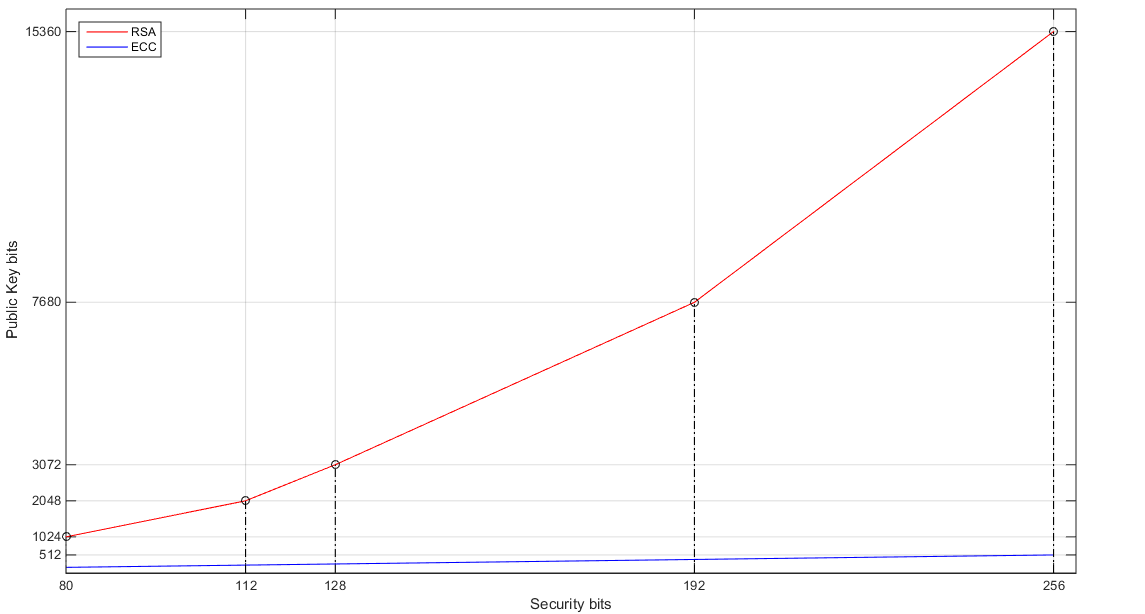
\includegraphics[scale=0.55]{RSAvECC_matlab}
% \caption{}
 \label{rsaveccpercent}
\end{figure}
Vogliamo dunque mostrare un ultimo confronto tra RSA ed ECC: a parit\`a di livello di sicurezza, mostriamo il numero di operazioni necessarie a risolvere il DLP e l'ECDLP mediante gli attacchi pi\`u efficaci considerati.
Chiamiamo ``\textit{L}" il relativo livello di sicurezza al quale facciamo riferimento. Per RSA il miglior algoritmo risolutivo necessita di $e^{\sqrt[3]{ln(n) \cdot ln( ln( n) )^2}}$ operazioni; per ECC abbiamo la $\rho$ di Pollard con $\sqrt{\ddfrac{\pi n}{2}}$ operazioni. Il valore detto $n$ rappresenta il numero $2^b$ ovvero il numero che otteniamo mediante chiavi da $b$ bit. Nella colonna $ECC/RSA$ si mostra un rapporto tra le operazioni necessarie ad entrambi gli algoritmi per risolvere il problema del logaritmo discreto.
\\
Prendiamo in considerazione anche il tempo di elaborazione dell'algoritmo per rompere il generico DLP: un anno MIPS corrisponde al numero di operazioni che vengono svolte in 365 giorni di attivit\`a da un singolo processore che lavora alla frequenza di 1 milione di operazioni al secondo. Tale numero corrisponde a $MIPS=3.1 \cdot 10^{13}$ operazioni totali. Gli anni MIPS necessari per il calcolo di $x$ operazioni sono calcolati come il rapporto $x / $\textit{MIPS}, vedasi a tal proposito le colonne \textit{MIPS RSA} e \textit{MIPS ECC}. La colonna \textit{MIPS ECC/RSA} non viene mostrata: passare da un valore della colonna \textit{ECC} al corrispettivo \textit{MIPS ECC} significa dividere secondo il coefficiente \textit{MIPS}, lo stesso concetto si applica per \textit{RSA} concludendo che il rapporto di operazioni \textit{ECC/RSA} corrisponda esattamente a quello in anni MIPS.
\begin{center}
\begin{tabular}{c |c |c |c |c |c }
& \multicolumn{3}{c|}{Operazioni} &\multicolumn{2}{c}{Anni MIPS}\\
\hline
L & RSA & ECC & ECC/RSA & RSA & ECC\\
\hline
80 & $3.8 \cdot 10^{13}$ & $1.5 \cdot 10^{24}$ & $3.9 \cdot 10^{10}$ &  1.2 & $4.7 \cdot 10^{10}$\\
112 & $1.9 \cdot 10^{18}$ & $6.5 \cdot 10^{33}$ & $3.4 \cdot 10^{15}$ &  $6.0 \cdot 10^{4}$ & $2.0 \cdot 10^{20}$\\
128 & $5.2 \cdot 10^{21}$ & $4.3 \cdot 10^{38}$ & $8.2 \cdot 10^{16}$ &  $1.6 \cdot 10^{8}$ & $1.3 \cdot 10^{25}$\\
192 & $6.0 \cdot 10^{31}$ & $7.9 \cdot 10^{57}$ & $1.3 \cdot 10^{26}$ &  $1.9 \cdot 10^{18}$ & $2.5 \cdot 10^{44}$\\
256 & $1.4 \cdot 10^{42}$ & $1.5 \cdot 10^{77}$ & $1.0 \cdot 10^{35}$ &  $4.4 \cdot 10^{28}$ & $4.7 \cdot 10^{63}$
\end{tabular}
\end{center}
Aver scelto l'algoritmo base della $\rho$ di Pollard non cambia molto la situazione rispetto la sua versione parallelizzata: colmare la differenza di operazioni tra i due problemi richiede tanti processori quanto il rapporto ECC/RSA. Solo per il livello minimo, 80 bit, si dovrebbero considerare circa 39 miliardi di processori attivi simultaneamente. 
\\
Quanto mostrato nella tabella costituisce un ulteriore incentivo verso la scelta della crittografia ellittica. Il livello medio di sicurezza, 128 bit, comporta dapprima un impiego di memoria nettamente inferiore in ECC rispetto RSA (solo l'8\% della lunghezza in bit) e, al tempo stesso, le operazioni da computare per risolvere l'ECDLP risultano $8.2 \cdot 10^{16}$ volte maggiori in confronto con il DLP. Il tempo di calcolo per rompere i due logaritmi discreti \`e notevole in entrambi i casi ma non possiamo fare affidamento su un tempo di $1.6 \cdot 10^{8}$ (RSA, 128 bit) per determinare tale algoritmo come \textit{crittograficamente sicuro} per gli anni futuri. Compatibilit\`a e retrocompatibilit\`a con dispositivi in uso in tutto il mondo sono fattori fondamentali nella scelta di un buon algoritmo di crittografia. L'importanza di mantenere chiavi ``\textit{piccole}" \`e fondamentale per mantenere RSA efficiente: trovare e moltiplicare due numeri primi molto grandi pu\`o causare una latenza eccessiva sui dispositivi meno performanti. Il risultato di quanto evidenziato \`e la deprecazione di RSA \cite{NIST key lenght} per il 31 Dicembre 2017.
\\
A confronto, chiavi pi\`u piccole per ECC consentono di velocizzare notevolmente i calcoli di generazione per la chiave privata: si fa infatti uso di un numero casuale $d$ scelto in un ampissimo intervallo. Ricordando che la chiave privata $d$ per algoritmi ellittici va presa nell'intervallo $[1, n-1]$ diamo un'idea di quanto ampia sia la scelta. Nello standard \cite{dss} la NIST raccomanda l'utilizzo di cinque curve diverse, ognuna per un differente livello di sicurezza. Tali curve sono denominate $P_{x}$ dove $x$ determina la pi\`u grande potenza di 2 utilizzata nell'esprimere la cardinalit\`a del campo primo $\mathbb{F}_p$:
\begin{align*}
 P_{192} &\to p=2^{192} - 2^{64}-1\\
 P_{224} &\to p=2^{224} - 2^{96}+1\\
 P_{256} &\to p=2^{256} - 2^{224}+ 2^{96}-1\\
 P_{384} &\to p=2^{384} - 2^{128}-2^{96}+2^{32}-1\\
 P_{521} &\to p=2^{521} -1
\end{align*}
La curva standardizzata $P_{192}$ ha equazione $y^2=x^3 -3x+b$ \cite{ec standard} con cardinalit\`a 
\begin{center}
$n=6277101735386680763835789423176059013767194773182842284081$
\end{center}
Ne consegue che scelta della chiave privata, per la curva pi\`u ``\textit{debole}" crittograficamente parlando, ricade nell'ampissimo intervallo $[1, 6.2\cdot 10^{58}]$.
\\
\\
Appurato ci\`o, nuovi algoritmi fanno uso di un numero detto \textbf{Seed} $S$ in base al quale vengono generati i coefficienti $a$ e $b$ per la curva. I seed sono generalmente identificati come ``\textit{nothing up my sleeve}": le prime cifre decimali della funzione seno applicata a numeri interi; le cifre iniziali del $\pi$; il numero di Nepero \textit{e}; il rapporto aureo e cos\`i via. Ci\`o che li rende numeri ``\textit{crittograficamente sicuri}" \`e potervi dare una giustificazione matematica. 
\\
Applicazioni del Seed si trovano nelle stesse curve standardizzate dal NIST; sebbene la presenza del coefficiente fisso $a=-3$, il parametro $b$ viene calcolato come segue: 
\begin{itemize}
    \item si sceglie un seed $s$ di lunghezza pari a 160 bit
    \item si calcola $c = $SHA1$(s)$ basato ovvero sull'output SHA1 del seed
    \item si calcola $b = \sqrt{-\ddfrac{27}{c}}$ mod$(p)$, detto $p$ l'ordine del campo $\mathbb{F}_p$
\end{itemize}
Le curve cos\`i costruite prendono la denominazione \textbf{Pseudo-Casuali}.
%
%
%
%
%
%
%
%
%
%
%
%
%
%
%
%
%
%
\section{Costruzione di Curve Ellittiche sicure}
Terminiamo lo studio riguardante la sicurezza offerta dalla crittografia ellittica indicando come avvenga la generazione di una curva ellittica crittograficamente sicura. I parametri che abbiamo utilizzato per descrivere gli algoritmi di crittografia e firma digitale mediante curve ellittiche fanno uso dei parametri pubblici
\begin{center}
$t=(a, b, p, G, n, h)$
\end{center}
ovvero i parametri $(a, b)$ della curva definita su di un campo primo $\mathbb{F}_p$, il punto generatore $G$ che identifica un sottogruppo $H$ di cardinalit\`a $n$ e cofattore $h$ tali per cui valga $\#H=nh$.
\\
Vogliamo ora determinare la scelta di tali parametri in accordo con i vari livelli di sicurezza $L \in \{80, 112, 128, 192, 256\}$.
\begin{enumerate}
 \item Per soddisfare la condizione di curva liscia dobbiamo imporre che $4a^3+27b^2 \ne 0$ mod$(p)$
 \item per tali coefficienti la curva deve avere cardinalit\`a $\#E \ne p$ per evitare che sia detta Anomala e suscettibile all'attacco di Smart (capitolo \ref{ecdlp conclusioni})
 \item l'ordine $n$ e la cardinalit\`a $p$ devono essere tali che, per ogni intero $B$ nell'intervallo $[1, 100)$, valga la relazione $p^B \ne 1$ mod$(n)$
 \item per essere resitente contro l'algoritmo di Pohlig-Hellman (capitolo \ref{poliwag}), l'ordine $n$ deve essere un grande numero primo. Mantenere vera tale affermazione implica che la relazione $\#E=nh$ sia verificata per un grande $n$ ed un, quanto possibile, piccolo cofattore $h$. Per questo motivo imponiamo la condizione $h \leq 2^{L / 8}$, dove $L$ rappresenta il livello di sicurezza per cui stiamo generando i parametri. Quanto pi\`u elevato il livello di sicurezza, tanto pi\`u piccolo dovr\`a essere il cofattore in rapporto ad $n$
 \item infine terminiamo imponendo una condizione sull'ordine $n$: i pi\`u grandi fattori primi di $n-1$ ed $n+1$ detti $v$, $w$, devono verificare le condizioni $log_n (v) > 19/20$ e $ log_n (w) > 19/20$
\end{enumerate}
Le condizioni esposte sono state prese in accordo alla ricerca della Certicom \cite{sec1}. 
\\
D'altronde pu\`o verificarsi che nonostante l'interlocutore Alice abbia generato in modo sicuro la curva, Bob voglia accertarsi della validit\`a dei parametri scelti. La validazione avviene come descritto di seguito:
\begin{enumerate}
 \item la cardinalit\`a $p$ del campo deve rispettare la sicurezza crittografica attribuita alla curva, percui bisogna avere 
 \begin{center}$
 \ceil{log_2(p)}=
 \begin{cases}
  192 & \text{se }L=80,\\
  2L & \text{se }80<L<256,\\
  521 & \text{se }L=256,\\
 \end{cases}$
 \end{center}
 inoltre, come definito durante la generazione dei parametri, deve valere \begin{center}
 $p^B \ne 1$ mod$(n)$, $\forall B\in [1, 100)$
 \end{center} 
 \item i parametri $(a, b)$ devono appartenere al campo $\mathbb{F}_p$ e verificare che la curva sia liscia, ossia $4a^3+27b^2 \ne 0$ mod$(p)$
 \item la cardinalit\`a $n$ deve corrispondere ad un numero primo, diverso da $p$
 \item le coordinate del generatore $G=(x_G, y_G)$ devono appartenere sia al campo $\mathbb{F}_p$ e sia alla curva verificando che valga $y_G^2=x_G^3+ax_G+b$ mod$(p)$. Un ulteriore controllo mira a determinare se l'ordine di $G$ sia effettivamente $n$ cercando di verificare l'uguaglianza $nG=\mathcal{O}$
 \item per il cofattore deve valere la condizione imposta durante la generazione dei parametri $h<2^{L / 8}$
 \item Infine bisogna verificare che la cardinalit\`a verifichi il teorema di Hasse per cui \begin{center}
 $\ceil{\, p+1-2\sqrt{p}\,} \leq \#E \leq \floor{\,p+1+2\sqrt{p}\,}$
 \end{center}
 oppure verificare il valore corretto di $\#E$ applicando l'algoritmo di Schoof.
\end{enumerate}
Un esito positivo per ogni condizione verifica la correttezza e la sicurezza crittografica dei parametri in uso.
%
%
%
%
%
%
%
%
%
\chapter{Conclusioni}
In questa tesi sono state evidenziate le curve ellittiche su campi primi e le loro applicazioni crittografiche. Dal confronto con i protocolli ElGamal, RSA e DSA, l'uso delle curve ellittiche permette grandi miglioramenti sia in termini di risorse utilizzate sia per la sicurezza che queste offrono.
%Nello studio che si \`e voluto portare avanti non ci si \`e soffermati sui campi binari, difatti le curve ellittiche su campi $\mathbb{F}_{2^m}$ trovano una ridotta applicazione in ambito crittografico seppur implementabili efficientemente su hardware come le smart card \cite{binary}. La formula che governa una curva ellittica di questo tipo si ottiene a partire dalla forma estesa di Tate-Weierstrass (formula \ref{Forma Estesa}), considerando un campo binario $\mathbb{F}_{2^m}$ ed applicando il cambio di coordinate  \begin{center}$x=a_1^2X+\ddfrac{a_3}{a_1}$,$y=a_1^3+\ddfrac{a_1^2a_4+a_3^2}{a_1^3}$\end{center}arrivando all'equazione\begin{gather} y^2+xy=x^3+ax^2+b\end{gather}
\\
\\
Sono stati analizzati alcuni algoritmi di risoluzione del problema del logaritmo discreto per le curve ellittiche riportando come questi siano possibili solo per determinate curve (anomale, supersingolari) o adatti ad ogni tipo di curva ma con alcuni grandi svantaggi (una hash table troppo grande da redigere per il BSGS, algoritmi probabilistici come quelli di Pollard).
\\
Numerosi enti quali NIST, Certicom, Brainpool, NSA hanno curato lo studio di questi attacchi e si sono occupati di redigere standard sulla scelta di curve ellittiche. NIST e Certicom risultano i due enti pi\`u attivi nelle problematiche attuali di performance e nel definire e proporre le curve oggi utilizzate in ECDH ed ECDSA. 
\\
\\
Concludiamo il discorso mostrando una curva ideata dal professor Daniel Julius Bernstein dell'universit\`a di Chicago: la \textbf{Curve25519}. 
\\
La curva \`e stata progettata per diminuire le operazioni svolte nella moltiplicazione scalare ed al tempo stesso mantenere un alto livello di sicurezza. Sebbene sia una curva ellittica per definizione, la forma in cui troviamo la curva viene detta \textit{forma di Montgomery}. Il passaggio \cite{ec2mont} da una curva ellittica $E:y^2=x^3+ax+b$ descritta su di un campo primo $\mathbb{F}_{p^m}$ alla sua forma di Montgomery $E^M: BY^2 =X^3+AX^2+X$ \`e possibile qualora vengano soddisfatte delle ipotesi: 
\begin{itemize}
      \item[-] la caratteristica del campo $\mathbb{F}_{p^m}$ deve essere diversa da 2, stiamo ancora una volta escludendo i campi binari
      \item[-] l'equazione $x^3+ax+b=0$ deve avere almeno una soluzione all'interno del campo $F_{p^m}$
      \item[-] il numero $3y^4+a$ deve avere soluzioni nel campo $F_{p^m}$
      \item[-] bisogna rispettare la relazione $B(A^2-4) \ne 0$ all'interno del campo $\mathbb{F}_{p^m}$.
\end{itemize}
L'equazione della Curve25519 \`e mostrata di seguito:
\begin{center}
$Y^2=X^3+486662X^2+X$ mod$(2^{255}-19)$
\end{center}
Due particolarit\`a della curva sono una sicurezza di 128 bit e l'impiego di chiavi crittografiche da 32 byte. La chiave pubblica non \`e un punto della curva ma la sua sola coordinata $x$: ci\`o permette di dimezzare le risorse necessarie all'invio ed alla conservazione in memoria della stessa. 
\\
Test effettuati dallo stesso Bernstein, riportati in \cite{curve25519 fast, speed table}, mettono a confronto la Curve25519 con numerose altre curve, tra le quali quelle standardizzate dal NIST. Si evidenziano quindi una sensibile riduzione nel numero di operazioni e nel tempo di calcolo necessari alla generazione delle chiavi crittografiche. 
\\
La base matematica ed i coefficienti scelti per la costruzione della Curve25519 identificano una curva non anomala, n\`e supersingolare risultando immune all'attacco di Smart; il grande numero primo scelto per la cardinalit\`a della curva offre grande protezione contro l'attacco di Pohlig-Hellman. Infine, come affermato dallo stesso Bernstein in \cite{curve25519 fast} l'implementazione della curva \cite{impl 25519} \`e immune da attacchi Side-Channel per via dell'uso della Montgomery Ladder.
\\
Si conclude dicendo che questa curva rappresenta un'ottima scelta per l'implementazione di protocolli crittografici basati sulla crittografia ellittica.
%
%
%
%
%
%
%
%
%
%
\chapter*{Ringraziamenti}
Il tempo trascorso in questi anni sembra corrispondere ad un attimo. Anni di studio, amicizia, difficolt\`a hanno contribuito a rendermi una persona pi\`u matura e capace di affrontare i problemi a testa alta. La scelta dell'ateneo \`e seguita da un consiglio di un mio grande amico, Luca, che non ha mai smesso di essere un grande punto di riferimento e consigli. Voglio ringraziarlo ancora una volta per l'amicizia, la pazienza e la costanza che ha messo in ogni cosa rendendola speciale. Un grazie allo stesso modo speciale lo devo a Chiara, per l'infinita gentilezza e attenzione che pone in ogni parola, per la calma con cui affronta le difficolt\`a e tutta l'amicizia e l'affetto che ha dimostrato in questi anni. Tra i tanti colleghi di universit\`a e di corso, Gianpaolo \`e stato un Amico, un compagno di banco e di studio; di avventure, risate e delle tante frustrazioni per gli esami. Sempre propenso ed impegnato nel risolvere le situazioni pi\`u difficili, senza mai far pesare i suoi sforzi, mi ha dato il coraggio e la forza di andare avanti e proseguire tutte le volte che stavo per cedere. Gabriele, compagno di corso anche lui, mi ha offerto spunti di riflessione e pensieri personali che mi hanno portato ad osservare la realt\`a di tutti i giorni sotto un'ottica nuova, influenzando positivamente e con ottimismo il mio modo di pensare. Devo un grazie ad Alessandro per avermi dato la fiducia e la determinazione a cambiare e completare gli studi; ed al suo infinito ottimismo. Ringrazio ancora una volta Benedetta per l'amicizia e per avermi aiutato in numerose occasioni, soprattutto per la disponibilit\`a quando non potevo rivolgermi ad altri.
\\
In particolare voglio ringraziare Simone, Daniele e tutta la loro famiglia per l'affetto e la disponibilit\`a dimostrati da sempre. Un secondo grazie a Simone per esser stato inseparabile nonostante la distanza e l'aver condiviso tantissime esperienze ed idee.
\\
Non posso dimenticare di ringraziare Leonardo per la pi\`u grande amicizia che abbia mai avuto. Lo ringrazio per avermi aiutato e dato consigli ogni giorno; per condividere con me cos\`i tante esperienze personali da rendere la nostra amicizia unica in assoluto; per aver trascorso anni in casa insieme ed avermi sempre sopportato con il sorriso. Soprattutto sento di doverlo ringraziare per avermi insegnato a farmi carico dei miei problemi ed a restare calmo e sereno di fronte le difficolt\`a che non sapevo affrontare.
\\
Arrivo quindi a ringraziare tutti i professori dell'ateneo, rivolgendo un sincero grazie al professor Di Stefano per avermi indicato l'argomento di tesi, per la pazienza portata ed il suo prezioso aiuto che mi ha permesso di completare questo studio con mia grande soddisfazione.
\\
\\
Ringrazio i miei genitori e le mie sorelle per ogni giorno e per l'opportunit\`a di studio datami. In particolare voglio ringraziare mio padre per aver avuto fiducia in me e la pazienza di aspettare fino a questo giorno. Infine vorrei ringraziare mia madre per avermi dato la possibilit\`a di giungere dove sono arrivato e dirle di aver mantenuto la promessa fatta tanti anni fa.










\bibliografia{tesi}
\begin{thebibliography}{99}

%1
\bibitem{curva3c}
  \emph{Enciclopedia Treccani},
  Istituto della Enciclopedia Italiana,
  1970.

%2
%--------------------%

%3
\bibitem{baseTheory_GT}
  James S. Milne,
  \emph{Group Theory}, 
  versione 3.14, 
  2017.
  
%4
  \bibitem{baseTheory_Groups}
  Mark Reeder,
  \emph{Notes on Group Theory},
  Addison Wesley, Massachusetts,
  2015.
  
%5
  \bibitem{anelli1}
  Karl-Heinz Fieseler,
  \emph{Groups, Rings and Fields},
  2010.
  
%6
  \bibitem{char_Ring}
  Robert B. Ash,
  \emph{Abstract Algebra: The Basic Graduate Year},
  Dipartimento di Matematica,
  Universit\`a di Illinois,
  revisione Febbraio 2011.
  
%7
  \bibitem{baseTheory_ProjSpace}
  Nigel Hitchin,
  \emph{Projective Geometry},
  Professore di Geometria,
  Universit\`a di Oxford,
  2003.
  
%8
  \bibitem{baseTheory_ProjSpace2}
  Ulf Persson,
  \emph{Projective Geometry},
  Dipartimento di Matematica,
  Chalmers Universit\`a di Tecnologie,
  1989.
  
%9
  \bibitem{baseTheory_Euclid2Proj_Space}
  Sonja Gorjanc,
  \emph{Extended Euclidean Plane - } 
  \url{http://www.grad.hr/geomteh3d/skripta/uvod_eng.html},
  traduzione in inglese a cura di Helena Halas e Iva Kodrnja,
  Universit\`a di Zagreb.
  
%10
  \bibitem{baseTheory_LineAtInfinity}
  Franz Lemmermeyer,
  \emph{Lecture Notes -}
  \url{http://www.fen.bilkent.edu.tr/~franz/ta/ta01.pdf},
  Professore di Matematica,
  2004.
  
%11
  \bibitem{baseTheory_CurvePianeCubiche}
  James W. Kiselik,
  \emph{Conic and Cubic Plane Curves},
  Dipartimento di Matematica,
  Universit\`a di Chicago,
  2015.

%12
  \bibitem{Wolfram}
  \url{WolframAlpha.com} per la consultazione delle seguenti definizioni: Curva ellittica, Punto K-Razionale, Legge di Gruppo per le curve ellittiche.
  
%13
  \bibitem{P Torsione 1}
  Geir Ellingsrud,
  \emph{Elliptic curves - Basics},
  Dipartimento di Matematica,
  Universit\`a di Oslo,
  2014.
  
%14
  \bibitem{P Torsione 2}
  Christine Croll,
  \emph{Torsion Points of Elliptic Curves Over Number Fields},
  Tesi di laurea breve in Matematica,
  Universit\`a del Massachusetts,
  2006.
  
%15
  \bibitem{Tate-Weier EQ}
  John Tate,
  \emph{The Arithmetic of Elliptic Curves},
   Dipartimento di Matematica,
   Universit\`a di Harvard,
  1973.
  
%16
  \bibitem{P_Torsione p9}
  Evan Dummit,
  \emph{Mathematical Cryptography part 5: Elliptic Curves in Cryptography},
   Dipartimento di Matematica,
   Universit\`a di Rochester,
  2016.
  
%17
  \bibitem{RSAp+q}
  R.L. Rivest, A. Shamir, and L. Adleman,
  \emph{A Method for Obtaining Digital
Signatures and Public-Key Cryptosystems}.
  
%18
  \bibitem{guide to ECC}
  Darrel Hankerson, Alfred Menezes, Scott Vanstone,
  \emph{Guide to Elliptic
Curve Cryptography},
   Casa Editrice ``Springer-Verlag",
  2004.

%19
  \bibitem{codifica messaggi su CE}
  Neal Koblitz, 
  \emph{A Course in
Number Theory
and Cryptography},
Dipartimento di Matematica, 
Universit\`a di Washington
   Seconda Edizione,
   1994.
  
%20
  \bibitem{Shattered}
  Google, 
  \url{http://shattered.io/},
esperimento condotto per verificare la possibilit\`a di collisione in SHA-1,
23 Febbraio 2017.
  
%21
  \bibitem{dss}
  NIST, 
  \emph{FIPS PUB 186-4 - Digital Signature Standard (DSS)},
  Categoria: Computer Security,
  Sottocategoria: Crittografia,
  Luglio 2013.
  
%22
  \bibitem{sony}
  BBC, 
  \url{http://www.bbc.com/news/technology-12116051},
  \emph{``iPhone hacker publishes secret Sony PlayStation 3 key"},
  06 Gennaio 2011.
  
%23
  \bibitem{ec standard}
  NIST, 
  \emph{Recommended Elliptic Curves For Federal Government Use},
  1999.
  
%24
  \bibitem{monico}
  Certicom, articolo:
  \emph{``Certicom Announces Elliptic Curve Cryptography Callenge Winner"},
  2004.

  
%25
  \bibitem{Certicom pollard p}
  Certicom,
  \emph{The Elliptic Curve Cryptosystem} - Remarks on the Security of the Elliptic Curve Cryptosystem,
  2000.

  
%26
  \bibitem{libro 900 pagine}
  William Stallings,
  \emph{Cryptography and Network Security: Principles and Practice},
  Quinta edizione,
  Pearson Editore.
  
%27
  \bibitem{ascii}
  Tabella ASCII - American Standard Code for Information Interchange,
  \url{http://www.asciitable.com/}.
  
%28
  \bibitem{NIST key lenght}
  NIST,
  \emph{``Transitions: Recommendation for Transitioning the Use of Cryptographic Algorithms and Key Lengths"},
  Special Publication 800-131A,
  Revision 1,
  \url{http://nvlpubs.nist.gov/nistpubs/SpecialPublications/NIST.SP.800-131Ar1.pdf},
  Novembre 2015.

%29
  \bibitem{nist key conf}
  NIST,
  \emph{``Recommendation for Key Management"},
  NIST Special Publication 800-57,
  Part 1, Revision 4,
  \url{http://nvlpubs.nist.gov/nistpubs/SpecialPublications/NIST.SP.800-57pt1r4.pdf},
  Gennaio 2016.

%30
  \bibitem{parall rho}
  Matthew Musson,
  \emph{``Attacking the Elliptic Curve Discrete Logarithm Problem"},
  Tesi di Laurea Magistrale delle Scienze Matematiche e Statistiche,
  Acadia University,
  2006.
  
%31
  \bibitem{pollard el-psy-kongru}
  J. M. Pollard,
  \emph{``Monte Carlo methods for index computation mod p"},
  Vol 32, Numero 143.

%32
  \bibitem{el-psy 2}
  Paul C. van Oorschot, Michael J. Wiener,
  \emph{``Parallel Collision Search with Cryptanalytic Applications"},
  1996.

%33
  \bibitem{supersingolare}
  Andrew Sutherland,
  \emph{``E18.783 - Elliptic Curves"},
  Dipartimento di Matematica,
  MIT,
  2017.
  
%34
  \bibitem{rho for poliwag}
  Mandy Zandra Seet,
  \emph{``ELLIPTIC CURVE CRYPTOGRAPHY - Improving the Pollard-Rho Algorithm"},
  Universit\`a di New South Wales,
  02 Novembre 2007.

%35
  \bibitem{libro 800 pagine}
  Alfred J. Menezes, Paul C. van Oorschot, Scott A. Vanstone,
  \emph{``Handbook of Applied Cryptography"},
  1996.
  
%36
  \bibitem{ev_curv1}
  Peter Novorney,
  \emph{``Weak Curves in Elliptic Curve Cryptography"},
  2010.

%37
  \bibitem{ev_curv2}
  N. P. Smart,
  \emph{``The Discrete Logarithm Problem on Elliptic Curves of Trace One"}.

%38
  \bibitem{sec1}
  Daniel R. L. Brown,
  \emph{``Standards for Efficient Cryptography 1 (SEC 1)"},
  versione 2.0,
  Certicom, 
  21 Maggio 2009.
  
%39
  \bibitem{binary}
  Daniel Hein,
  \emph{``Elliptic Curve Cryptography ASIC for Radio Frequency Authentication"},
Gratz University of Technology,
  2008.

%40
  \bibitem{curve25519ecdh}
  Daniel Julius Bernstein,
  \url{``https://cr.yp.to/ecdh.html"},
Professore di Matematica,
Eindhoven University of Technology
  2005.
  
%41
  \bibitem{ec2mont}
  Katsuyuki Okeya, Hiroyuki Kurumatani, Kouichi Sakurai,
  \emph{``Elliptic Curves with the Montgomery-Form
and Their Cryptographic Applications"},
Professore di Matematica,
Universit\`a di Illinois, Chicago 
  2005.
  
%42
  \bibitem{safecurves}
Daniel J. Bernstein, Tanja Lange,
\emph{``SafeCurves: choosing safe curves for elliptic-curve cryptography"},
\url{https://safecurves.cr.yp.to}, 
22 Gennaio 2017.

%43
  \bibitem{brainpool}
  Manfred Lochter,
  \emph{``ECC Brainpool Standard Curves and Curve Generation"},
versione 1.0,
19 Ottobre 2005.

%44
  \bibitem{dlp fast1}
  Jonathan Katz, Yehuda Lindell,
  \emph{``Introduction to Modern Cryptography"},
seconda edizione,
2014.

%45
  \bibitem{dlp fast2}
  Andrew Odlyzko,
  \emph{``Discrete logarithms over finite fields"},
Universit\`a del Minnesota,
2012.

%46
  \bibitem{curve25519 fast}
  Daniel J. Bernstein,
  \emph{``Curve25519: new Diffie-Hellman speed records"},
Universit\`a di Chicago,
2006.

%47
  \bibitem{speed table}
  Daniel J. Bernstein,
  \url{``https://cr.yp.to/ecdh/reports.html"} - \emph{``Speed reports for elliptic-curve cryptography"},
Universit\`a di Chicago.

%48
  %\bibitem{ed curves}  Harold M. Edwards,  \emph{``A normal form for elliptic curves"},Bulletin of the american mathematical society,09 Aprile 2007.


%49
  \bibitem{impl 25519}
  Daniel J. Bernstein,
  \url{``https://cr.yp.to/ecdh.html"} - \emph{``A state-of-the-art Diffie-Hellman function"},
Universit\`a di Chicago.

%50
  \bibitem{schoof}
  Gregg Musiker,
  \emph{``Schoof's Algorithm for Counting Points on $E(\mathbb{F}_q)$"},
Universit\`a del Minnesota,
Professore associato di Matematica,
7 Dicembre 2005.

%51
  \bibitem{rho speed1}
  Paul C. van Oorschot, Michael J. Wiener,
  \emph{``Parallel Collision Search with Cryptanalytic Applications"},
1996.

%52
  \bibitem{rho speed2}
  Silje Christensen, Simen Johnsrud,
  \emph{``Speeding up the Pollard’s Rho algorithm"},
1996.






%99
  \bibitem{immagini}
  Immagini generate grazie a 
  \begin{itemize}
      \item[-] \url{https://cdn.rawgit.com/andreacorbellini/ecc/920b29a/interactive/reals-add.html}
      %\item[-] \emph{Andrea Corbellini - Elliptic Curve Cryptography: finite fields and discrete logarithms}
      \item[-] \url{https://www.desmos.com/}
      \item[-] Matlab
  \end{itemize}
  
  
  

\end{thebibliography}


\afterpage{\blankpage}
%
%
%
%
%
%
%
%
%
%
%\appendice
%\chapter{prima appendice}
%
%
%
%
%
%
%
%
%
%
%\chapter{seconda appendice}
%
%
%
%
%
%
%
%
%
%
\end{document}